\documentclass[journal=jacsat,manuscript=article]{achemso}

\usepackage[version=4]{mhchem}
\usepackage{graphicx}
\usepackage{subcaption}
\usepackage{siunitx}
\usepackage{xr}
\usepackage{hyperref} 
\usepackage{cleveref}

\externaldocument[prefix]{output}

\captionsetup[subfigure]{skip=1pt,singlelinecheck=false}
\newcommand*\mycommand[1]{\texttt{\emph{#1}}}
\author{Nianhan Tian}
\affiliation[Georgia Institute of Technology]
{School of Chemical and Biomolecular Engineering, Georgia Institute of Technology, Atlanta, Georgia 30318 USA}

\author{Ehsan Abbasi}
\affiliation[Texas Tech University]
{Department of Chemical Engineering, Texas Tech University, Lubbock, Texas 79409 USA}

\author{Haldrian Iriawan}
\affiliation[Massachusetts Institute of Technology]
{Department of Materials Science \& Engineering, Massachusetts Institute of Technology, Cambridge, Massachusetts 02139 USA}

\author{Paul Kohl}
\affiliation[Georgia Institute of Technology]
{School of Chemical and Biomolecular Engineering, Georgia Institute of Technology, Atlanta, Georgia 30318 USA}

\author{Gerardine G. Botte}
\affiliation[Texas Tech University]
{Department of Chemical Engineering, Texas Tech University, Lubbock, Texas 79409 USA}

\author{Yang Shao-Horn}
\affiliation[Massachusetts Institute of Technology]
{Department of Materials Science & Engineering, Massachusetts Institute of Technology, Cambridge, Massachusetts 02139 USA}

\author{Andrew J. Medford}
\affiliation[Georgia Institute of Technology]
{School of Chemical and Biomolecular Engineering, Georgia Institute of Technology, Atlanta, Georgia 30318 USA}
\email{ajm@gatech.edu}

\title{Electrochemical stability of metal and oxide catalysts in the presence of nitrogen ligands}

\abbreviations{IR,NMR,UV}
\keywords{American Chemical Society, \LaTeX}

%%%%%%%%%%%%%%%%%%%%%%%%%%%%%%%%%%%%%%%%%%%%%%%%%%%%%%%%%%%%%%%%%%%%%
%% The manuscript does not need to include \maketitle, which is
%% executed automatically.
%%%%%%%%%%%%%%%%%%%%%%%%%%%%%%%%%%%%%%%%%%%%%%%%%%%%%%%%%%%%%%%%%%%%%
\begin{document}
%%%%%%%%%%%%%%%%%%%%%%%%%%%%%%%%%%%%%%%%%%%%%%%%%%%%%%%%%%%%%%%%%%%%%
%% The abstract environment will automatically gobble the contents
%% if an abstract is not used by the target journal.
%%%%%%%%%%%%%%%%%%%%%%%%%%%%%%%%%%%%%%%%%%%%%%%%%%%%%%%%%%%%%%%%%%%%%
\begin{abstract}
\end{abstract}

\section{Introduction}
The growing global population continues to drive demand for ammonia-based fertilizers, placing additional pressure on the nitrogen cycle. Traditionally, nitrogen-based fertilizers are produced from ammonia synthesized through the Haber-Bosch process, which supports the agricultural productivity \cite{Schloegl2003CatalyticStory}. However, the Haber–Bosch reaction operates at high temperatures (250 to 400~$^\circ$C) and pressures (100 to 300~bar) \cite{Smil1999DetonatorExplosion,Erisman2008HowWorld, Lim2021Ammonia2050,Verleysen2021HowStorage}, relies on fossil-derived hydrogen, and leaves a significant carbon footprint \cite{Liu2022ProspectsFixation, Smil1999DetonatorExplosion,Suryanto2021NitrogenShuttle}.

Waste streams from agriculture and municipal wastewater offer an underused alternative source of reduced nitrogen \cite{ChipocoHaro2024ElectrocatalystsConversion,Adebayo2004EvaluationFingerlings,Mulchandani2016RecoverySludges}, which constitutes 15\% of total nutrients in the sludge \cite{Xiao2020ProteinReview, Thomsen2017ChangesSludge}. The organic matter dissolved in sludge includes nucleic acids, humic acids, proteins, and polysaccharides \cite{Jung2002RecoverabilityWastewater}. Electrochemical methods, such as the electrolysis of waste-activated sludge (EWAS), offer a more sustainable pathway to valorize dissolved organics while mitigating environmental impacts operating at ambient temperatures \cite{Botte2024InnovativeRecovery,Vedharathinam2014ExperimentalMedium,Alvarez-Pugliese2024PerspectivesWaste, Zeng2019ElectrochemicalSulfide,Ye2016ElectrochemicalProduction}.

Existing EWAS methods often rely on high applied voltages (5–30 V) to drive the oxidation and conversion of nitrogen species in sludge. During these highly oxidative potentials, reactive oxygen species and form and compete with nitrogen intermediates for active sites on catalysts. While Jafari et al. \cite{JafariElectrochemicalProduction} demonstrated that lower-voltage electrolysis can reduce side reactions, they could result in lower current densities ($<$30~mA~cm$^{-2}$) and ammonia yields ($<$5 mass\%) \cite{Zhao2022AAmmonia}. To reduce electrode fouling, particularly from passivation by organic polymers in sludge \cite{Wang2014InCatalysts}, and to maintain the activity of redox-sensitive catalysts such as NiOOH, which is known to degrade rapidly under operating conditions \cite{JafariElectrochemicalProduction}, many systems adopt non-constant current and potential by alternating polarity \cite{Schotten2021AlternatingSynthesis, Hall2020SustainablePrinciples, Chandrasekar2008PulseApplications, Larson2012CurrentReview, Adamson2017ProbingVoltammetry}. This potential cycling technique helps mitigate surface fouling, restore catalyst surface integrity and reaction efficiency by using surfaces evenly and preventing the buildup of metal dendrites that could cause short-circuiting. 

However, these alternating conditions impose new challenges on electrode stability. Materials must endure not only strong oxidative potentials but also the mechanical and chemical stresses from repeated redox cycling. These challenges are further compounded by the high pH of typical EWAS operations, which can accelerate corrosion and dissolution \cite{Sanchis2022NitrateOverview, Popov2015ThermodynamicsCorrosion, Kapaka2010ElectrochemicalElectrode, Mucalo2004InSolutions, Aksu2001ElectrochemistrySolutions, OConnor2018ElectrochemicalSolutions}. Additionally, competition between nitrogen oxidation reactions and the oxygen evolution reaction (OER) further compromises catalytic performance \cite{Li2021Ru-DopedNitrate, Wang2022ElectrochemicalOxidation, Dai2020ElectrochemicalOxides}.

In nitrogen-rich environments, reactive nitrogen species such as ammonia (\ce{NH3}), glycine, and cyanide (\ce{HCN}) can coordinate with metal sites to form soluble complexes, promoting leaching and surface degradation \cite{Bjerrum1957StabilitySubstances, Meng1996PrinciplesReview, Wang2022AmmoniaSystem}. Except molybdenum, most transition metals are susceptible to leaching due to their tendency to form water-soluble complexes with nitrogen-containing ligands \cite{Meng1996PrinciplesReview, Ma2021ALeaching, Wang2020Reduction-ammoniacalSalts, Li2025Glycine-mediatedStudy}. Although such metal-ligand interactions have been extensively characterized in hydrometallurgical systems \cite{Han1974AMMONIA-AMMONIUMNODULES, Bhuntumkomol1982TheSolutions, Azadi2021SustainableGlycine, Oraby2020GoldPermanganate, Sarvar2023ApplicationStructure, SPARROW1995CyanideApplications, Akcil2015PreciousReview, Wang2022AmmoniaSystem, Ma2021ALeaching, Wang2020Reduction-ammoniacalSalts, Li2025Glycine-mediatedStudy}, these studies differ significantly from EWAS conditions, where ligand concentrations are lower, and applied potential is alternative between oxidative and reducing potentials.


Pourbaix diagrams, also known as electrochemical phase diagrams or potential–pH diagrams, are widely used tools in materials chemistry for predicting the thermodynamic stability of metals, oxides, ions, and hydroxides in aqueous environments \cite{PourbaixAtlasSolutions, Huang2015ElectrochemicalCalculations, McCafferty2010ThermodynamicsDiagrams}. By mapping stable phases as functions of pH and electrode potential, these diagrams reveal dissolution, passivation, and oxidation regimes for understanding corrosion behavior and materials design \cite{Stack2005BridgingDiagrams, Pourbaix1973LecturesCorrosion, Fontana1987CorrosionCompany}. Traditionally, they have been developed for pure metals and their interactions with hydrogen and hydroxide ions \cite{Huang2017ImprovedCompounds, Wang2020PredictingFunctional, Cao2020E-pHLaterite} to predict the thermodynamics of electrochemical reactions. To address this gap, Pourbaix diagrams have been extended in hydrometallurgical studies to include nitrogen-rich ligands (e.g., \ce{NH3}, glycine, \ce{CN^-}) for understanding metal leaching under high-temperature, and high-ligand-concentration conditions \cite{Meng1996PrinciplesReview, NasuhaYahya2019ThermodynamicDiagram, Barragan2021LeachingOptimization, OConnor2018ElectrochemicalSolutions, Seke2006EffectSphalerite}. However, the direct application of these diagrams to electrocatalysis remains limited, particularly under the lower-concentration, ambient-temperature conditions relevant to EWAS.

Existing computational Pourbaix diagrams typically address pure metals \cite{PourbaixAtlasSolutions, Cao2020E-pHLaterite, HongOn, Meng1996PrinciplesReview}, and often neglect the stability domains of mixed-metal oxides or alloy phases \cite{Ding2018ElectrochemicalStates}. Although Pourbaix diagrams for common alloys such as stainless steel have been developed \cite{Cubicciotti1985TheSteel, Beverskog1999PourbaixIron-Chromium-Nickel}, diagrams for binary and ternary alloy systems remain limited \cite{Dong2021ElectrochemicalData, Ding2018ElectrochemicalStates}. Since alloyed materials provide a balance between stability and activity, expanding the Pourbaix framework to include alloyed systems and their interactions with nitrogen ligands is essential for designing sustainable electrodes in practical EWAS conditions.


Experimental Pourbaix construction relies on measured chemical potentials \cite{PourbaixAtlasSolutions, Pourbaix1973LecturesCorrosion, Beverskog1999PourbaixIron-Chromium-Nickel}, but accurate data can be difficult to obtain due to sample complexity and characterization challenges \cite{Huang2017ImprovedCompounds}. First-principles methods now enable diagram construction from DFT-calculated Gibbs free energies of solids combined with experimental ion data \cite{Wang2020PredictingFunctional, Lopez2023ComputationalStudies, Liu2024ReversiblePH, Ding2018ElectrochemicalStates, Huang2015ElectrochemicalCalculations, Persson2012PredictionStates, Patel2019EfficientCompounds, Oses2018AFLOW-CHULL:Analysis}. Large materials databases such as the Materials Project \cite{Ong2013PythonAnalysis, Singh2017ElectrochemicalMaterials, Jain2011FormationCalculations, Montoya2015TheoreticalSplitting, Singh2019RobustDiscovery} now make high-throughput stability screening feasible. While DFT functionals may carry functional-dependent errors, such as the overbinding of O$_2$ in PBE, SCAN with Hubbard $U$ corrections has improved agreement with experimental oxide thermodynamics \cite{Wang2020PredictingFunctional}.


To address the underexplored interplay of nitrogen ligands, pulsing applied potentials, and alloying effects, we extend the Pourbaix diagram methodology to evaluate the thermodynamic stability of transition metals and their alloys in nitrogen-rich environments. We focus on a representative set of pure metals, Ni, Cu, Pd, Pt, Au, Ti, and selected binary alloys, revealing that Ti–Ni and Pd–Au may offer a promising tradeoff between stability and reactivity. We incorporate metal-ligand complexation with \ce{NH3}, glycine, and \ce{CN^-}, and examine wide potential and pH ranges to approximate electrochemical conditions. Together, these analyses establish thermodynamic stability as a key material screening criterion, providing a computational framework to guide the rational design of durable electrode materials for sustainable electrochemical nitrogen recovery.


\section{Methods}
\subsection{Pourbaix Diagram Construction}
Pourbaix diagrams were constructed to map the thermodynamic stability regions of bulk metals/alloys and their metal-ligand complexes in the presence of nitrogen-containing ligands at concentrations in the range expected to be present in EWAS.
%under electrolysis of waste activated sludge (EWAS) potentials in basic environment. 

Free energies of bulk metals were obtained from the Materials Project database \cite{Jain2013TheInnovation}, based on generalized gradient approximation (GGA) density functional theory (DFT) calculations. Free energies for aqueous ligands and metal-ligand complexes were calculated from equilibrium constants sourced from standard thermochemical handbooks \cite{Wagman1982TheUnits, Smith1989CriticalConstants, Bard2017StandardSolution, Bjerrum1957StabilitySubstances} and literature \cite{Meng1996PrinciplesReview, Azadi2019DataComplexes, Aviles2022ExploringNH3, Oraby2023SelectiveSolutions, Harrington2005DeterminationIon}. We focus here on metal elements that are commonly used as electrode materials and those where metal-ligand complex stabilities are available: Au, Cu, Ni, Co, Mg, Mn, Ti, Zn, Ag, Cd, Sr, Pt, Pd, and Fe. The aqueous ligands considered in this study include \ce{NH3-}, glycine, and \ce{CN-}. The targeted experimental potential ranges from -2.0 to 2.3 V (vs RHE) and the pH ranges from 11.5 to 13.5, but Pourbaix diagrams are constructed over a broader range for reference.


The diagrams were constructed based on the framework introduced by previous studies \cite{PourbaixAtlasSolutions, Huang2017ImprovedCompounds,Huang2015ElectrochemicalCalculations,Singh2017ElectrochemicalMaterials,Patel2019EfficientCompounds,Persson2012PredictionStates, Ding2018ElectrochemicalStates, Thompson2011PourbaixSystems} at 298.15 K. All reaction species, i.e., metals, alloys, oxides, aqueous ions and ligands, and water, are connected by their corresponding redox or acid-base reactions. Then the reaction chemical potentials are derived from equilibrium relationships between species, using the Nernst equation as a function of applied potential and pH.

For a general redox reaction:

\begin{equation} \label{eq:reaction}
aA + h\text{H}^+ + z\text{e}^- \leftrightarrow bB + \text{H}_2\text{O}
\end{equation}

The Nernst equation is:

\begin{equation} \label{eq:nernst}
E = E^\circ - \frac{k}{z} \log \left(\frac{[A]^a}{[B]^b}\right) - \frac{k \cdot h}{z} \, \text{pH},
\end{equation}

where \( E \) is the cell potential under non-standard conditions, \( E^\circ \) is the standard electrode potential, and \( k = \frac{RT}{F \ln 10} \). \( A \) and \( B \) are the activities of the reactants and products, and \( z \) is the number of electrons transferred. \( a \), \( b \), and \( h \) are the stoichiometric coefficients of the reactants, products, and protons, respectively.

Aqueous ion activities are approximated to be their concentration and are assumed to be \SI{1e-4}M \cite{Huang2017ImprovedCompounds, Wang2020PredictingFunctional, Patel2019EfficientCompounds, Thompson2011PourbaixSystems}. For ligands such as \ce{NH3}, glycine, and \ce{CN^-}, we apply a fixed representative concentration for each species based on experimentally relevant conditions. These concentrations are held constant throughout the Pourbaix analysis and are noted in the captions of each diagram. This approach allows for direct comparison with experimental systems and avoids introducing concentration-dependent variability into the stability trends.

For alloy Pourbaix diagrams involving multiple elements, all candidate alloy phases are generated from valid stoichiometric combinations of the relevant elemental entries available from the Materials Project \cite{Jain2013TheInnovation}. These combinations must satisfy the compositional constraint specific to the system under consideration (e.g. Ni:Ti = 1:1) \cite{Thompson2011PourbaixSystems}. To manage the computational complexity of this enumeration, the number of alloying elements is restricted to two. This enables systematic exploration of alloy stability within the compositional space relevant to each Pourbaix diagram while maintaining tractable scaling. 
% It is important to note that different compositional constraints can yield different Pourbaix diagrams, as the relevant free energies can vary depending on the reference stoichiometry.



The Pourbaix diagrams were generated by evaluating the chemical potentials of all species across a finely spaced potential-pH grid (4000 $\times$ 4000 points) and identifying the most thermodynamically stable species at each grid point. The thermodynamic stability of each species was calculated by comparing chemical potentials at each grid point across the potential-pH space. Stability regions were identified for bulk metals, aqueous ions, and metal-ligand complexes. 


\subsection{Incorporation of Nitrogen Ligands}

To extend the Pourbaix framework to systems containing nitrogen-based ligands (\ce{NH3}, glycine, and \ce{CN-}), ligand concentrations are represented as pLigand in \ref{eq:pligand} and incorporated into pH-dependent mass balance equations, assuming that the sum of the concentrations of protonated and deprotonated species is kept constant. For example, the dissociation equilibrium of \ce{NH3} (\ref{eq:NH3 equilibrium}) indicates the relationship between pH and p\ce{NH3} via \ref{eq:pNH3}:

\begin{equation} \label{eq:NH3 equilibrium}
\ce{NH4+} \leftrightarrow \ce{NH3} + \ce{H+}
\end{equation}

\begin{equation} \label{eq:pNH3}
\text{pNH}_3 = -\log \left([\text{NH}_3]_{\text{tot}}\right) + \log \left(1 + 10^{pK_a - pH} \right), \quad pK_a = 9.26 \text{ \cite{NationalCenterforBiotechnologyInformation2025PubChemAmmonia}}
\end{equation}

Similarly, anionic glycine and \ce{CN-} concentrations were calculated using \ref{eq:pGly} and \ref{eq:pCN}, respectively:
\begin{align} \label{eq:pGly}
\text{pGly} &= -\log \left([\text{Gly}_{\text{total}}]\right) + (pK_{a_1} - pH) \nonumber \\
&\quad + \log \left(1 + 10^{pH - pK_{a_1}} + \frac{1}{10^{pH - pK_{a_2}}} \right), \nonumber \\
&\quad pK_{a_1} = 2.37, \quad pK_{a_2} = 9.8 \text{ \cite{2025PubChemGlycine.}}
\end{align}
\begin{equation} \label{eq:pCN}
\text{pCN}^- = -\log \left([\text{CN}^-]_{\text{tot}}\right) + \log \left(1 + 10^{pK_a - pH} \right), \quad pK_a = 9.2 \text{ \cite{USEPA1980AmbientCyanides}}
\end{equation}
\begin{equation} \label{eq:pligand}
\text{pligand} = -\log[\text{ligand}].
\end{equation}

The interdependence of pH and ligand concentration (e.g., due to \ce{NH3} equilibrium in \ref{eq:NH3 equilibrium}) was modeled using these equations, which also include the assumption that ligand concentrations are unaffected by other ligands or external factors. For example, when both \ce{NH3} and \ce{CN-} were present, their equilibrium concentrations were treated as independent functions of pH.


Although cyanide is not deliberately introduced in EWAS systems, it is included in selected Pourbaix analyses to provide a conservative estimate of metal stability under conditions relevant to EWAS. Cyanide may arise as a transient intermediate during the electrochemical oxidation of organic nitrogen species \cite{Oraby2020GoldPermanganate, Chen2013AdsorptionStudy, Huerta1997ElectrochemicalPt111, Sandoval2011AdsorptionStudy}, and prior spectroscopic studies have shown that \ce{CN^-} can be electrochemically oxidized to cyanate under certain conditions \cite{Paulissen1992InfraredConditions, Hinman1986FourierElectrodes, Kitamura1986OxidationSpectroscopy, Chen2013AdsorptionStudy}.
As a strong-field ligand with a high affinity for transition metals, cyanide can significantly influence metal speciation and dissolution behavior. Moreover, due to its extreme toxicity and environmental impact \cite{xing2018simple, mekuto2016integrated, bruger2018volatilisation}, considering \ce{CN^-} in the Pourbaix framework provides a precautionary evaluation of electrode stability, particularly in worst-case scenarios involving ligand-induced leaching.


\section{Results and discussion}

\subsection{Thermodynamic screening of pure metals}
We performed thermodynamic screening of a range of pure metals to evaluate their stability under EWAS-relevant conditions. The complete set of metals screened, including Ni, Cu, Au, Pd, Pt, Ti, Co, Mg, Mn, Zn, Ag, and Fe, under ammonia and glycine ligand concentrations, is shown in \Cref{fig:metal_pourbaix_collage_1,fig:metal_pourbaix_collage_2,fig:metal_pourbaix_collage_3}. In each diagram, the stability of species is represented by their chemical potential as a function of pH and applied potential. At any point on the diagram, only the thermodynamically most stable species is shown, and the boundaries between regions indicate redox transitions such as metal dissolution or oxide formation. Dissolution regions, where aqueous metal ions or metal-ligand complexes are most stable, are shaded in blue, pink, and purple. Regions of immunity and passivation, where the metal or its oxide is stable, are colored green and yellow. The electrochemical conditions relevant to EWAS (pH 11.5–13.5 and potential -2 to 2 V vs. RHE) are highlighted by a green box in each figure.
%%%%%%%%%%%%%%%%%%%%%%%%%%%%%%%%% Collage of Pourbaix Diagrams %%%%%%%%%%%%%%%%%%%%%%%%%%%%%%%%%
\begin{figure}[htbp]
\centering
\makebox[\textwidth][c]{%g
        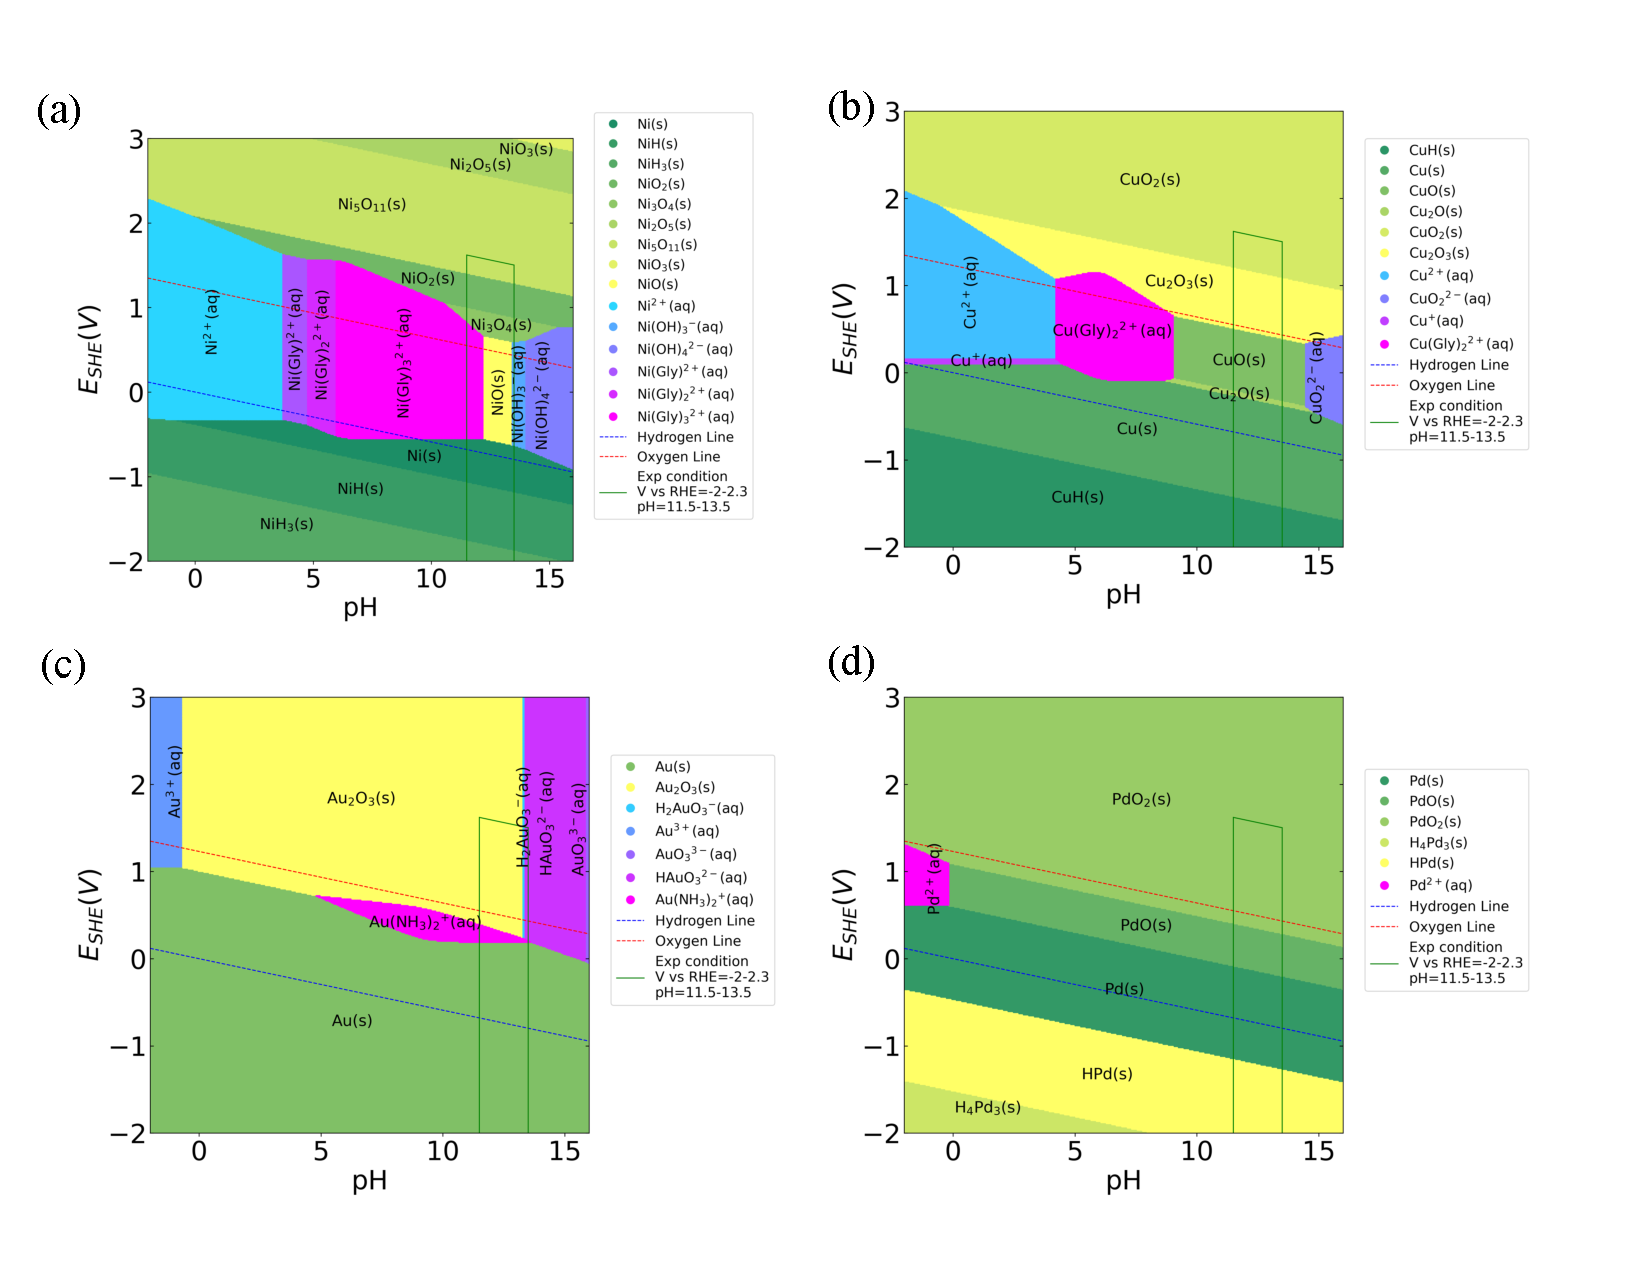
\includegraphics[width=1.1\textwidth]{Figures/pourbaix_diagrams/metal_pourbaix_collage_1.pdf}}
\caption{Metal Pourbaix diagrams: (a) Ni, (b) Cu, (c) Au, (d) Pd, with $\text{ion activity}=\num{1e-4}$M, $[\ce{NH3}]_{initial}= 0.02$M, $[\text{Gly}]_{initial}=0.005$M. The green box indicates the experimental condition at an applied potential of -2 to 2V vs RHE, pH = 11.5 to 13.5.}
\label{fig:metal_pourbaix_collage_1}
\end{figure}

\begin{figure}[htbp]
\centering
\makebox[\textwidth][c]{%g
        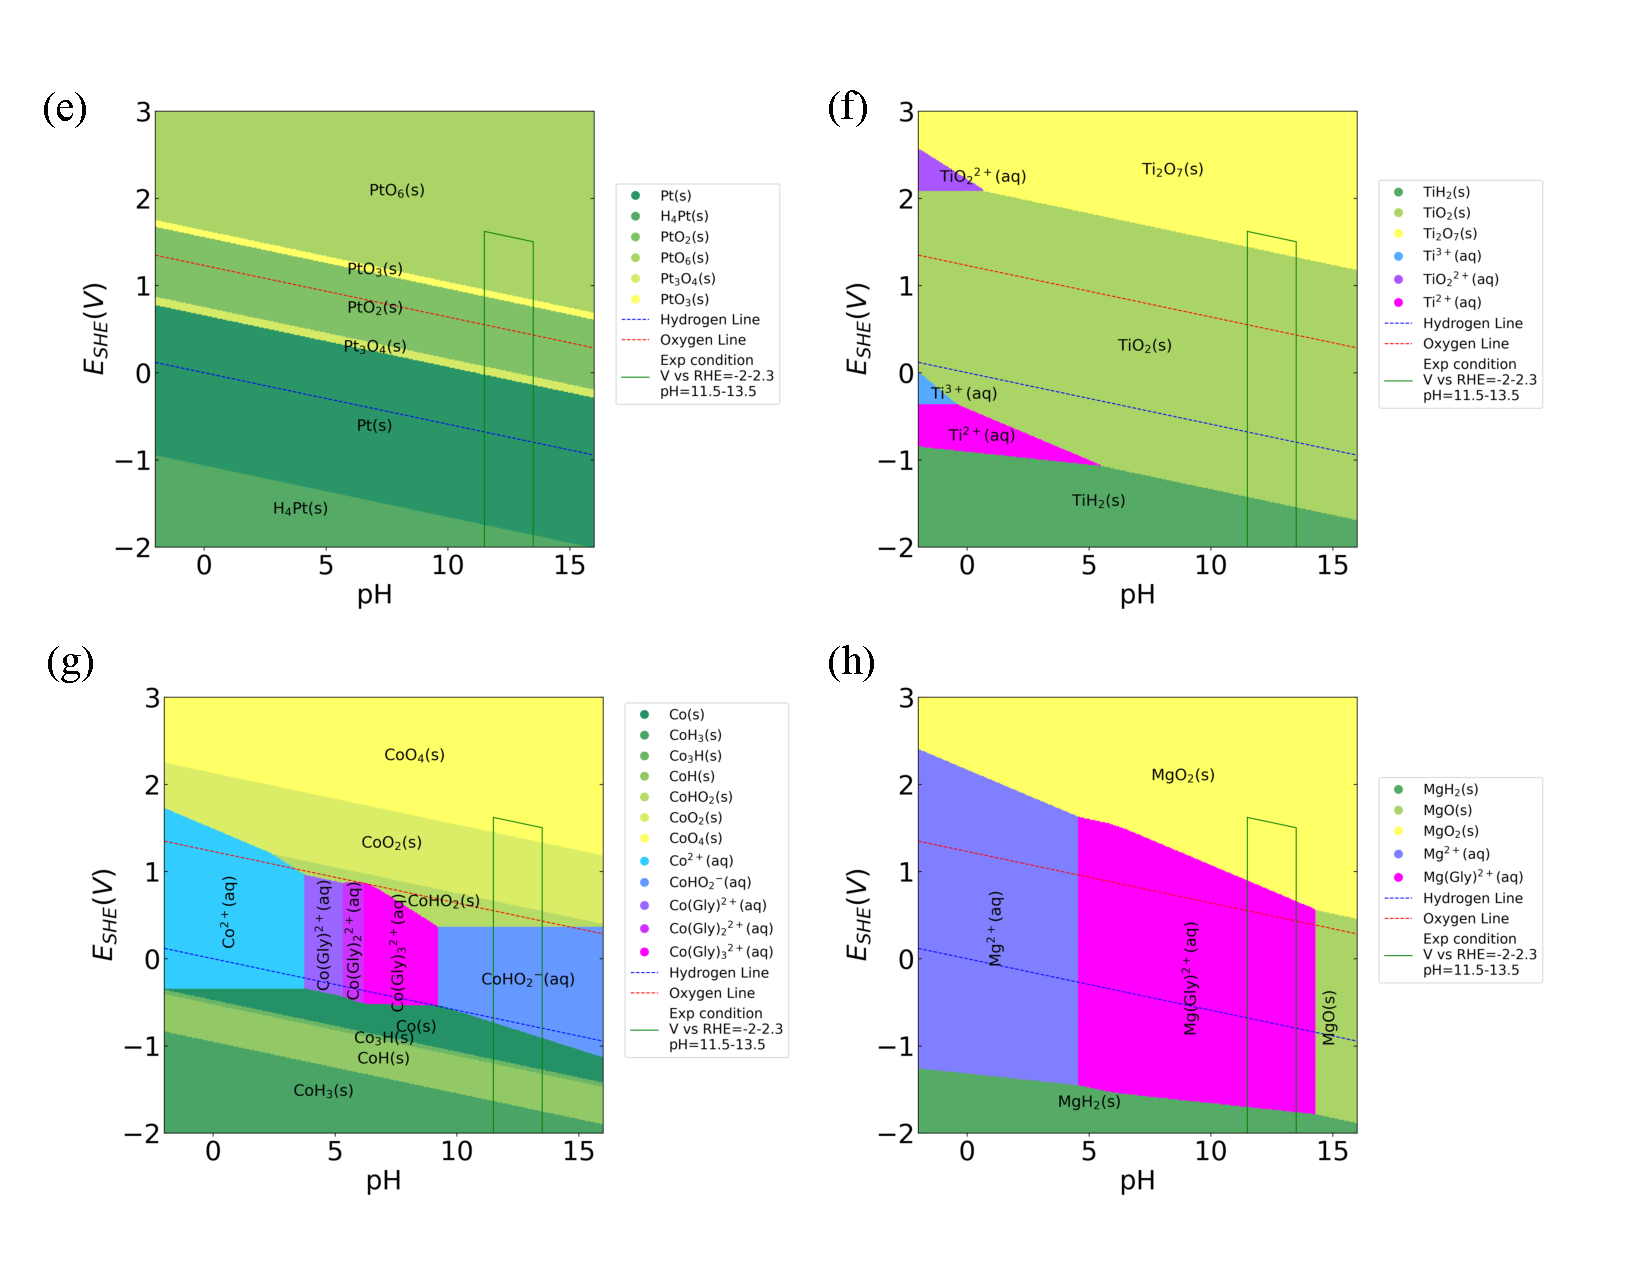
\includegraphics[width=1.1\textwidth]{Figures/pourbaix_diagrams/metal_pourbaix_collage_2.pdf}}
\caption{Metal Pourbaix diagrams: (a) Pt, (b) Ti, (c) Co, (d) Mg, with $\text{ion activity}=\num{1e-4}$M, $[\ce{NH3}]_{initial}= 0.02$M, $[\text{Gly}]_{initial}=0.005$M. The green box indicates the experimental condition at an applied potential of -2 to 2V vs RHE, pH = 11.5 to 13.5.}
\label{fig:metal_pourbaix_collage_2}
\end{figure}

\begin{figure}[htbp]
\centering
\makebox[\textwidth][c]{%g
        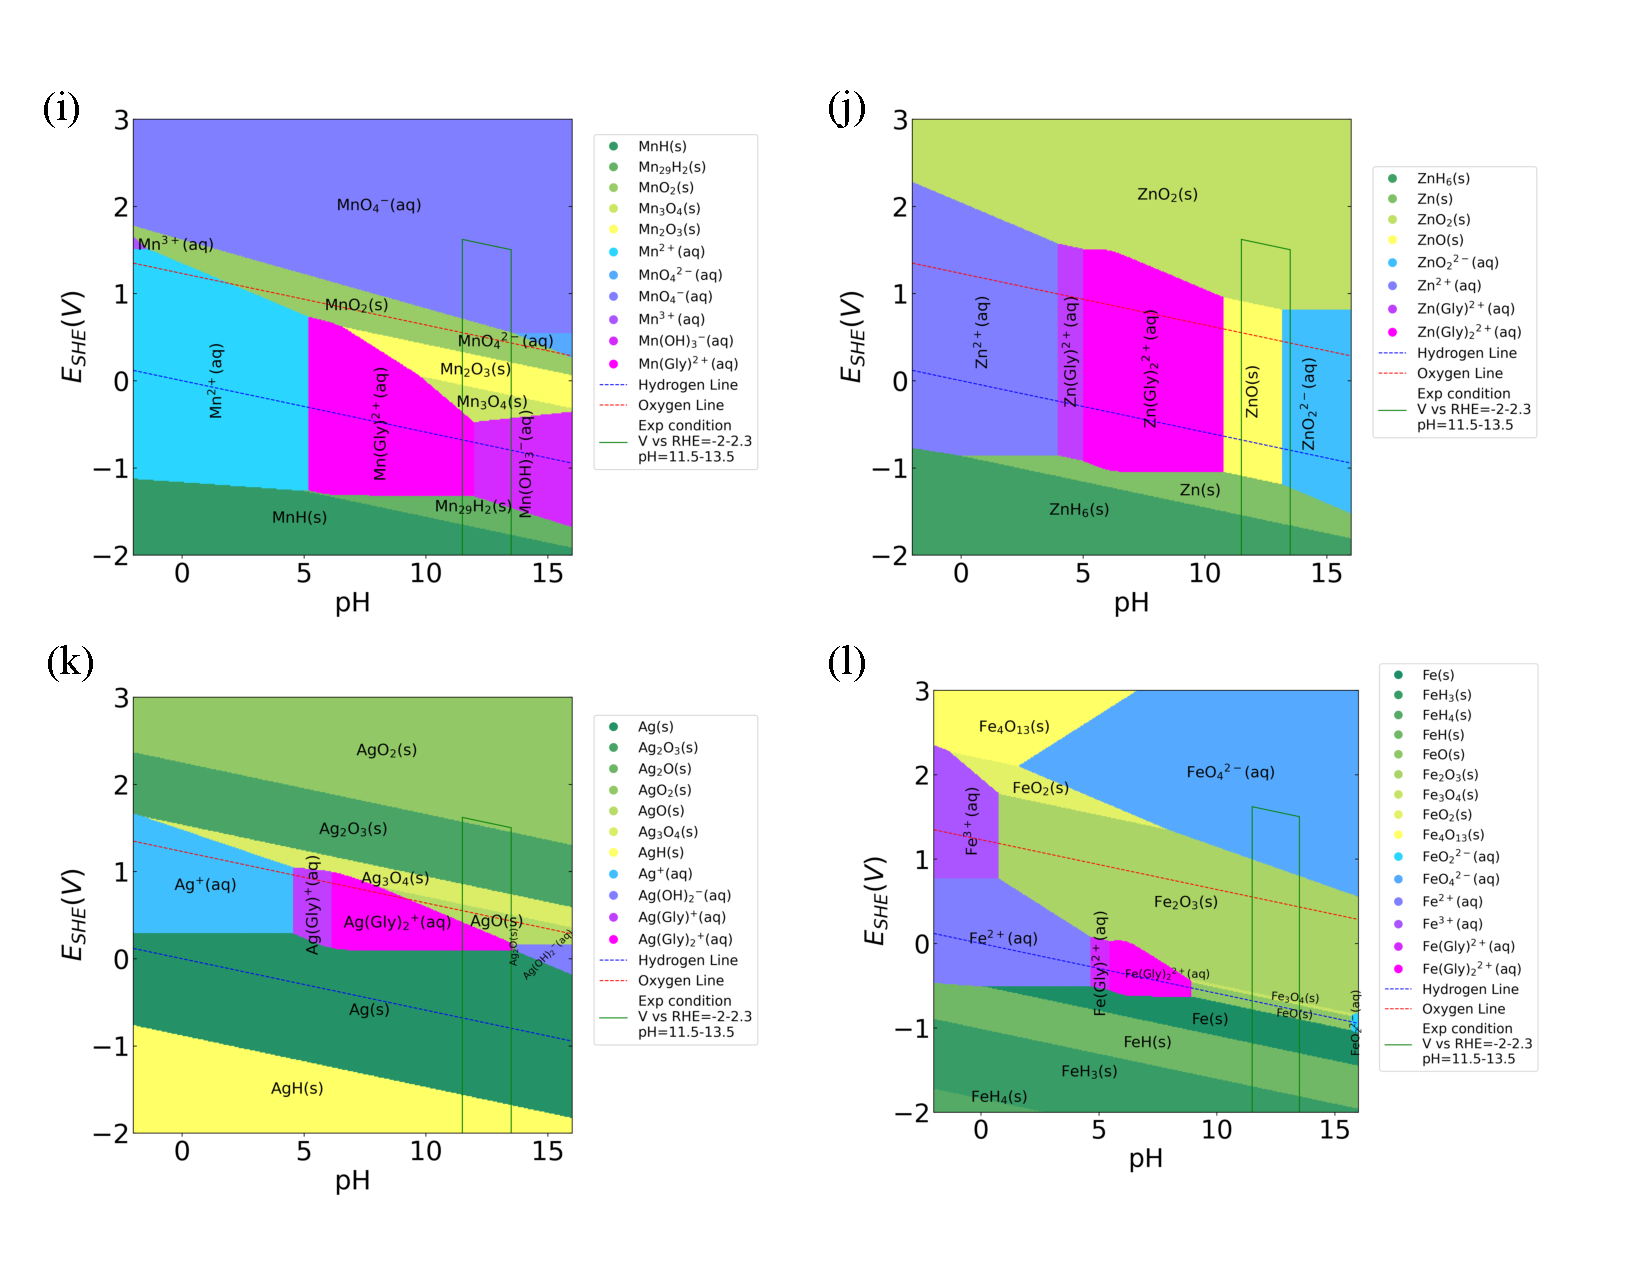
\includegraphics[width=1.1\textwidth]{Figures/pourbaix_diagrams/metal_pourbaix_collage_3.pdf}}
\caption{Metal Pourbaix diagrams: (a) Mn, (b) Zn, (c) Ag, (d) Fe, with $\text{ion activity}=\num{1e-4}$M, $[\ce{NH3}]_{initial}= 0.02$M, $[\text{Gly}]_{initial}=0.005$M. The green box indicates the experimental condition at an applied potential of -2 to 2V vs RHE, pH = 11.5 to 13.5.}
\label{fig:metal_pourbaix_collage_3}
\end{figure}
%%%%%%%%%%%%%%%%%%%%%%%%%%%%%%%%%%%%%%%%%%%%%%%%%%%%%%%%%%%%%%%%%

A general trend can be observed: those metals that tend to form stable aqueous ions (such as Ni, Cu, Au, Co, Mg, Mn, Zn, Ag, and Fe) also exhibit strong tendencies to form glycine and hydroxide complexes. In contrast, Pd, Pt, and Ti show bulk or oxide phase stability that is relatively unaffected by the presence of ammonia and glycine at an aqueous ion concentration of \SI{1e-4}M.

Metals like Ni, Cu, Au, Zn, and Ag display stable oxide phases under some experimentally relevant conditions. However, their glycine complexes are also thermodynamically stable in other relevant regions, often sharing a phase boundary with the oxide phase. Although the exact mechanism of dissolution of metallic phases in ligand-rich environments is not fully understood, it is proposed that metal dissolution proceeds through intermediate oxide formation, with dissolved oxygen acting as an oxidant \cite{Liao2012EffectsCopper, Ihnfeldt2008EffectNanohardness}. These metal oxides then react with ligands to form stable aqueous complexes \cite{Broeksma2023EvaluatingBoards, Du2004EffectIons, Ihnfeldt2008EffectNanohardness}. At lower pH, the dissolution of metals by ammonia and glycine decreases, consistent with the reduced thermodynamic stability of neutral ammonia and anionic glycine under less alkaline conditions \cite{Broeksma2023EvaluatingBoards}. Co, Mg, Mn, and Fe also form stable oxide phases in the EWAS-relevant region, while their hydroxide or glycine complexes become increasingly stable under alkaline and oxidative conditions.

Among the candidates, Ti-based materials were identified as the most stable across the full range of electrochemical potentials and pH values considered. This stability is primarily due to the spontaneous formation of a passive, thermodynamically stable \ce{TiO2} layer, which protects the underlying Ti metal from further oxidation \cite{Kuromoto2007TitaniumVoltages}. However, \ce{TiO2} is a wide band-gap semiconductor (3.2 eV for anatase and 3.0 eV for rutile) \cite{Earle1942TheDioxide, Bendavid1999StructuralDeposition}, and suffers from low conductivity \cite{Wu2014High-performanceApproach}. To address this limitation, structural modifications, such as alloying with conductive metals or doping with nonmetallic impurities, have been explored to enhance charge transport by increasing the concentration of charge carriers \cite{Zheng2011FacilePhenol, Hahn2009SemimetallicNanotubes}.

To further elucidate the trends observed in the thermodynamic screening, we analyze the stability and behavior of selected metals individually, under EWAS-relevant conditions with a focus on how their stability changes under EWAS-relevant conditions when little cyanide concentration (\SI{1e-4}M) is introduced. While cyanide is not typically added to EWAS systems, it may be generated as a transient species via the oxidation of amino acids like glycine. Across multiple systems, we find that even low cyanide concentrations can cause significant dissolution by stabilizing metal-cyanide complexes. Therefore, the use of metal electrodes that are susceptible to \ce{CN^-} dissolution should be approached with caution and a thorough understanding of the reaction mechanism.


\subsubsection{Nickel (Ni) Stability and Corrosion Behavior}
Nickel and its metal oxide and oxyhydroxide forms have been studied as electrode materials in hydrogen and oxygen evolution reactions, nitrogen-containing waste valorization, and urea electrolysis \cite{Wang2014InCatalysts, Yan2012NickelElectro-oxidation, Vedharathinam2012UnderstandingMedium, Coyle2025NovelCarbon, JafariElectrochemicalProduction, LiraGarciaBarros2025ImpactElectrolyzer, Wang2020Non-precious-metalAdvances} due to its catalytic activity and low cost. The Pourbaix diagrams for Ni (\Cref{fig:Ni_Pourbaix}) reveal distinct regions of immunity, passivity, and susceptibility to dissolution, which are strongly influenced by the presence of nitrogen-containing ligands. 

In nitrogen-free aqueous environments (\Cref{fig:Ni_Pourbaix_H2O}), Ni remains resistant to dissolution across a broad range of pH values up to 13 and applied potentials as high as 2~V vs. RHE. However, in the presence of glycine (\ref{fig:Ni_Pourbaix_NH3_Gly}), Ni forms thermodynamically stable complexes such as \ce{[Ni(Gly)_3]^{-}}. This behavior is consistent with literature reports showing that nitrogen-containing ligands serve as effective lixiviants for nickel extraction in hydrometallurgical systems \cite{Meng1996PrinciplesReview, Yao2021SelectivePhosphide, Ma2021ALeaching}. 

The inclusion of cyanide (\ref{fig:Ni_Pourbaix_NH3_Gly_CN}) further expands the dissolution region. Even at low concentrations (e.g., \num{1e-4}~M), \ce{[Ni(CN)_4]^{2-}} becomes the thermodynamically favored species across a wide range of pH, from 7 to 15, and potentials from -0.5 to 1.5V vs RHE. While cyanide is not initially present in most EWAS scenarios, its transient formation as a byproduct of glycine oxidation has been reported. Thus, Ni dissolution via cyanide complexation is a plausible corrosion pathway under pulsing redox conditions used in EWAS. However, the extent of this process will depend on the kinetics and competition with other reactions. Furthermore, because nickel and its dissolution products are toxic \cite{Bhattacharya2009CyanideTreatment}, Ni electrodes should be carefully tested for dissolution under operating conditions.


% The Pourbaix diagram for Ni (\ref{fig:Ni_Pourbaix}) reveals distinct immunity, passivity, and corrosion regions, which are significantly influenced by the presence of nitrogen-containing ligands. In pure aqueous environments (\ref{fig:Ni_Pourbaix_H2O}), Ni remains corrosion-resistant at oxidative potentials up to 2~V vs. RHE and pH values as high as 13. However, in the presence of glycine (\ref{fig:Ni_Pourbaix_NH3_Gly}), Ni forms stable complexes such as \ce{[Ni(Gly)_3]^{-}}, leading to dissolution. This thermodynamic stability of Ni-ammine and Ni-glycine complexes agrees with the literature that N-ligands solution is an effective lixiviant for nickel extraction \cite{Meng1996PrinciplesReview, Yao2021SelectivePhosphide, Ma2021ALeaching}. The effect of cyanide (\ref{fig:Ni_Pourbaix_NH3_Gly_CN}) is even more pronounced. Even at low concentrations (e.g., \num{1e-4}~M), the formation of \ce{[Ni(CN)_4]^{2-}} becomes thermodynamically favorable across a wide range of potential and pH values relevant to EWAS. Given that EWAS reactors operate under pulsing conditions that alternate between reductive and oxidative potentials, Ni corrosion via cyanide complexation is likely. Furthermore, because nickel and its dissolution products are toxic \cite{Bhattacharya2009CyanideTreatment}, Ni electrodes should be avoided in EWAS applications where ligand-rich or nitrogen-rich environments are present.

%%%%%%%%%%%%%%%%%%%%%%%%%%%%%%%%% Ni %%%%%%%%%%%%%%%%%%%%%%%%%%%%%%%%%
\begin{figure}[htbp]
    \centering
    \begin{subfigure}[b]{0.32\textwidth}
        \subcaption{}\label{fig:Ni_Pourbaix_H2O}
        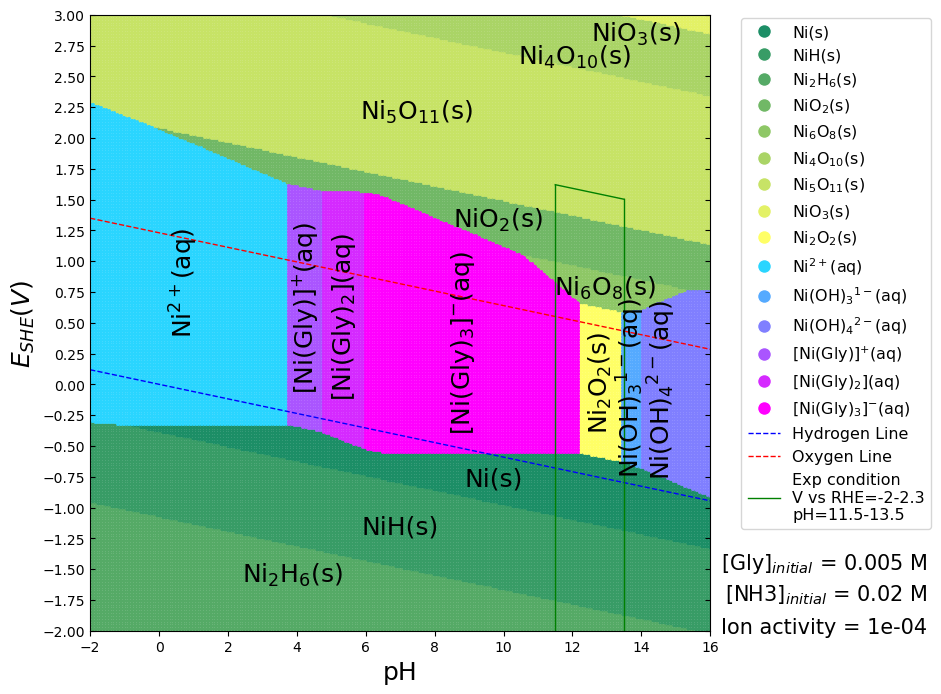
\includegraphics[width=\textwidth]{Figures/pourbaix_diagrams/Ni-NH3-H2O_activity=1e-04_[NH3]=0.02M_[Gly]=0.005M_[CN]=0.png}
        % \par\medskip
    \end{subfigure}
    \hfill
    \begin{subfigure}[b]{0.32\textwidth}
        \subcaption{}\label{fig:Ni_Pourbaix_NH3_Gly}
        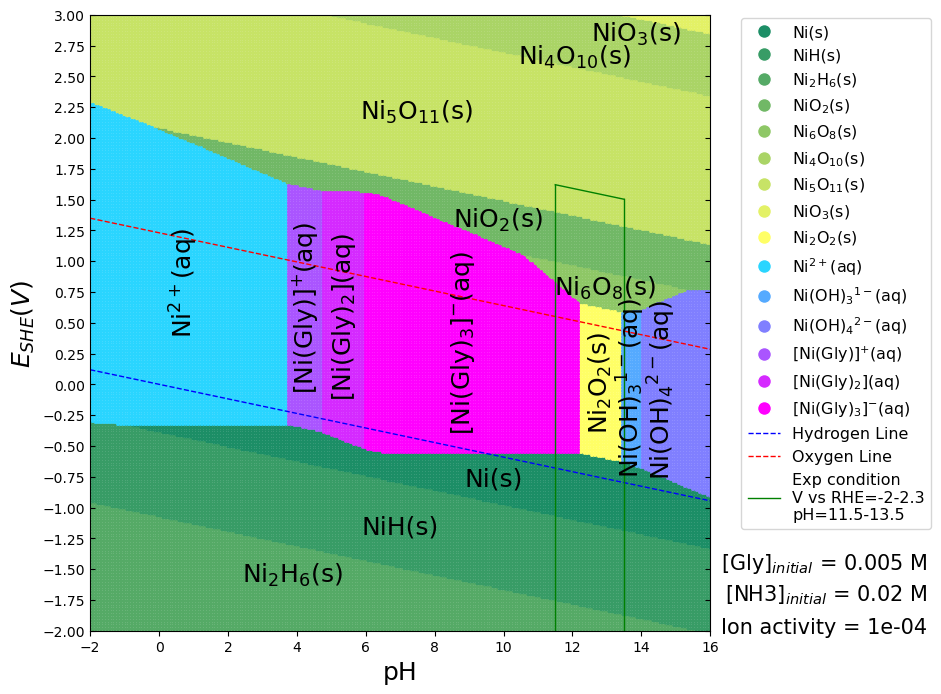
\includegraphics[width=\textwidth]{Figures/pourbaix_diagrams/Ni-NH3-H2O_activity=1e-04_[NH3]=0.02M_[Gly]=0.005M_[CN]=0.png}
        % \par\medskip
    \end{subfigure}
    \hfill
    \begin{subfigure}[b]{0.32\textwidth}
        \subcaption{}\label{fig:Ni_Pourbaix_NH3_Gly_CN}
        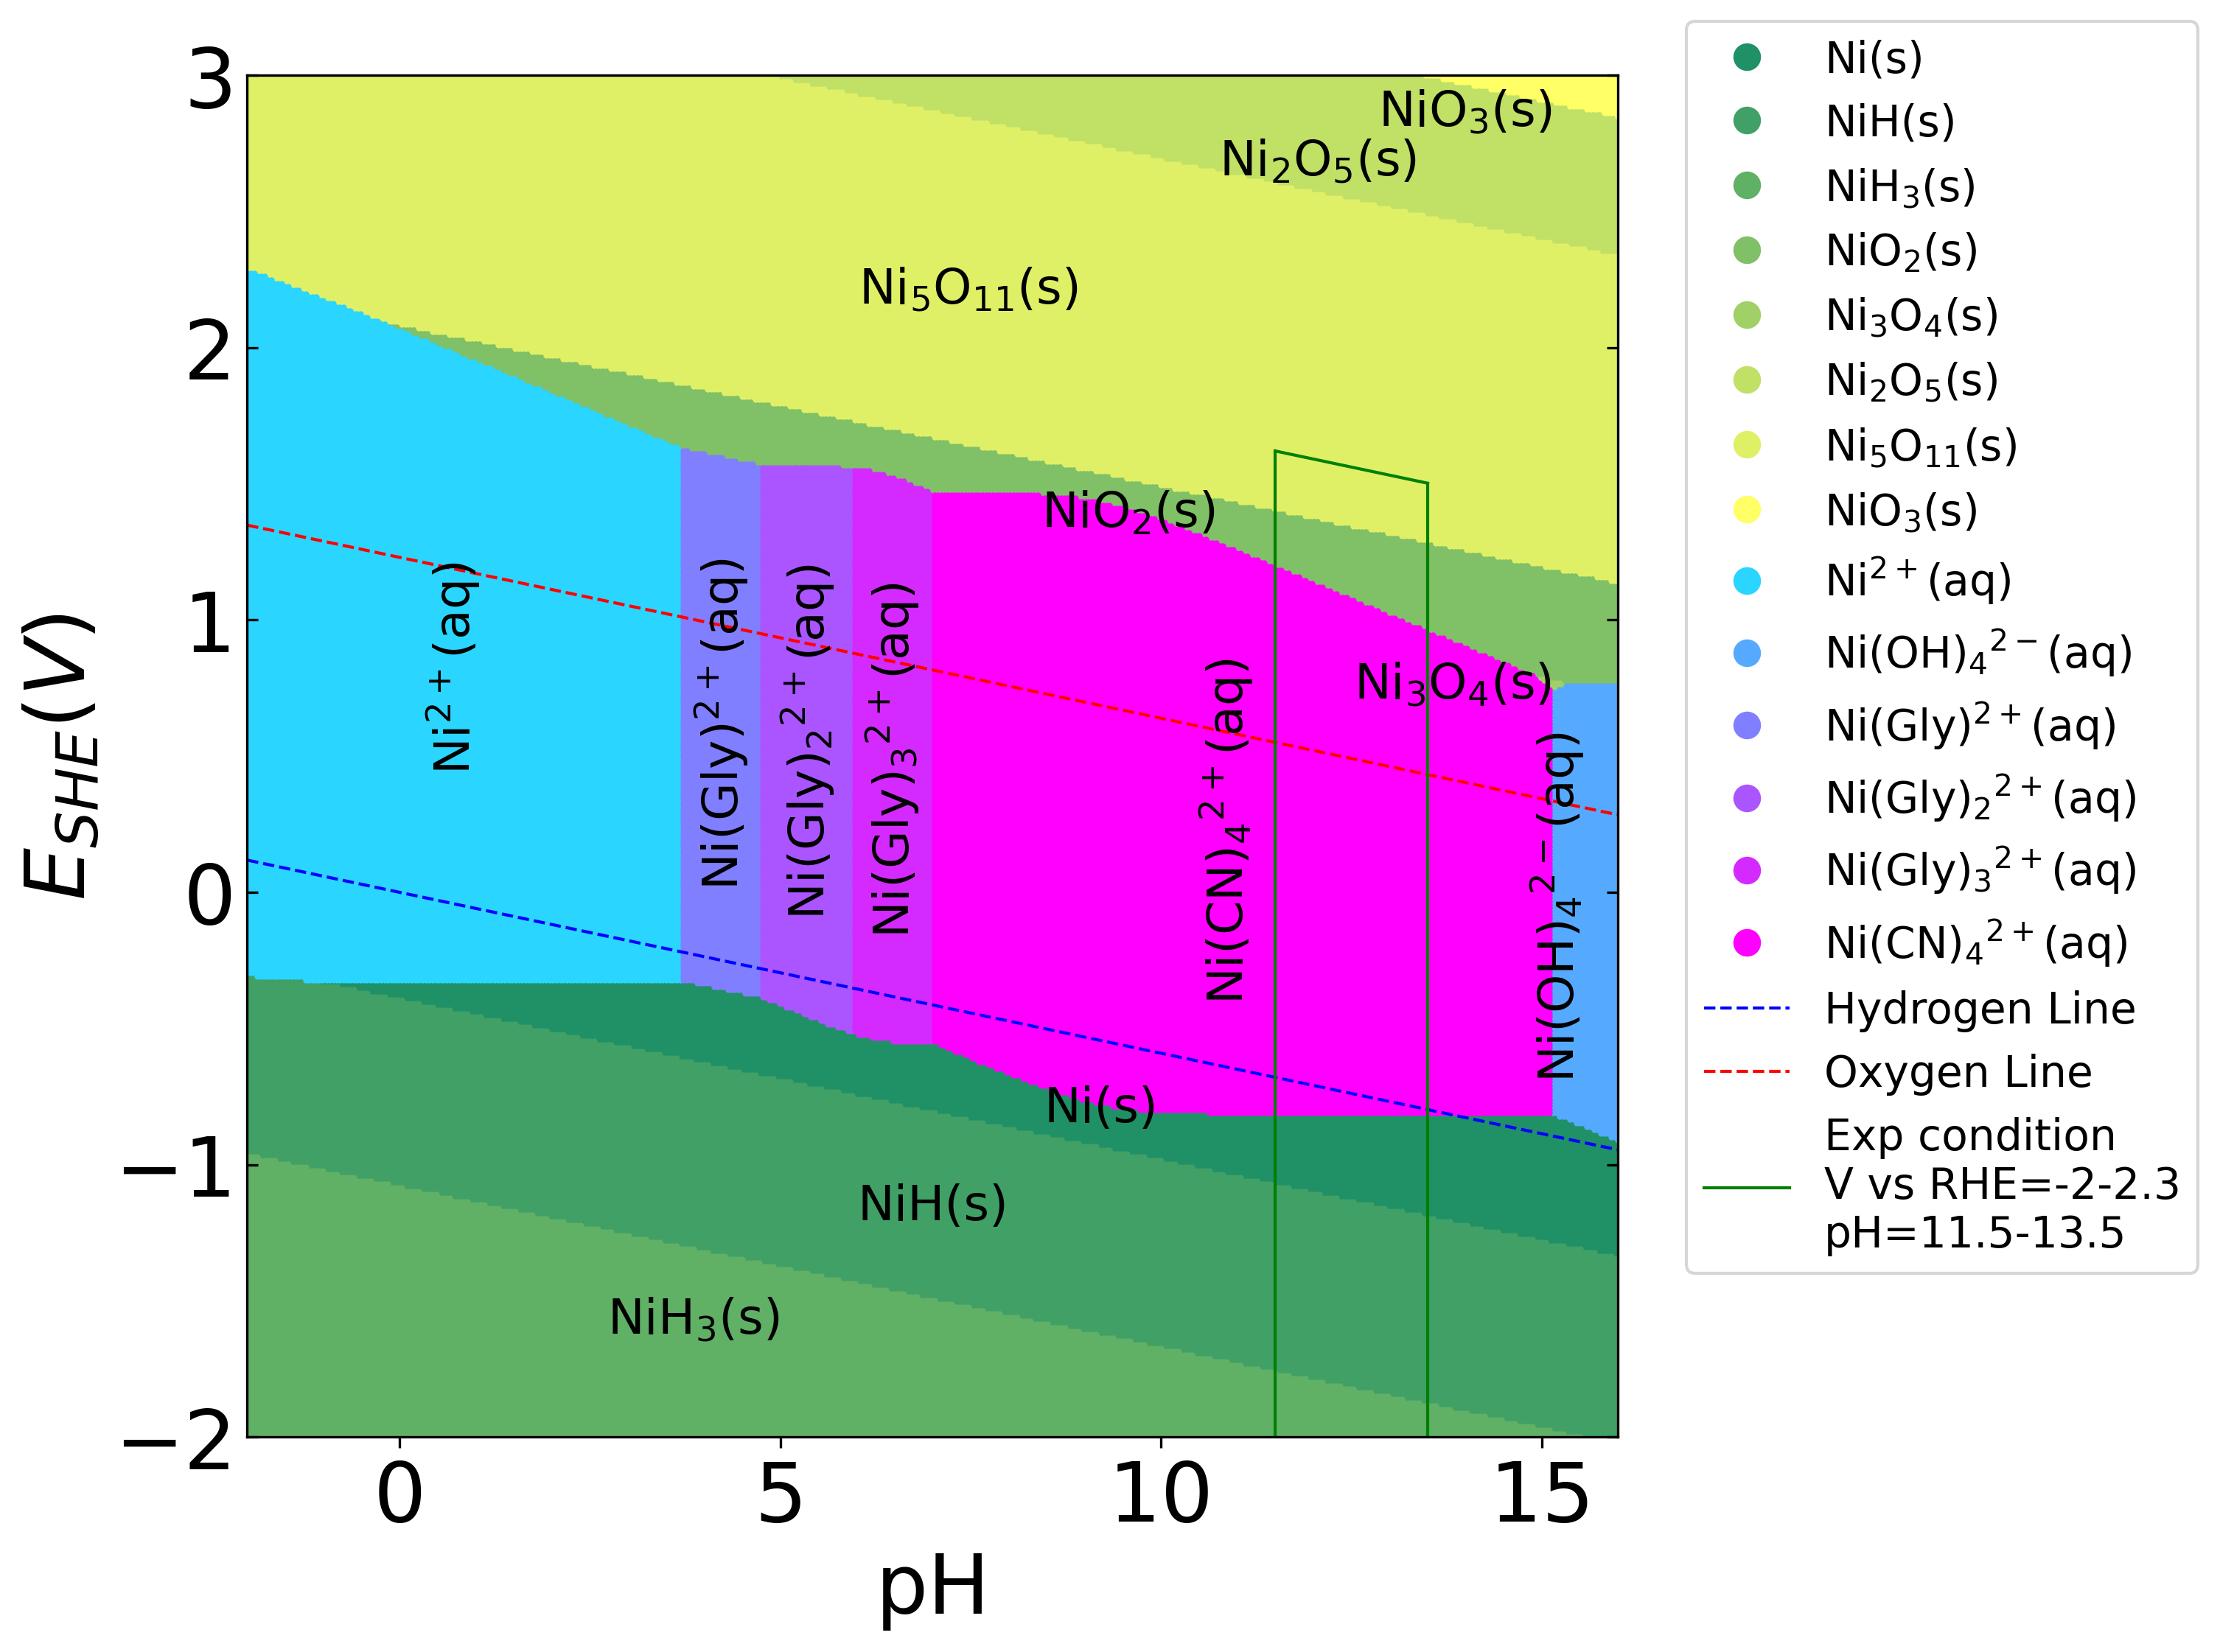
\includegraphics[width=\textwidth]{Figures/pourbaix_diagrams/Ni-NH3-H2O_activity=1e-04_[NH3]=0.02M_[Gly]=0.005M_[CN]=0.0001.png}
        % \par\medskip   
    \end{subfigure}
    \caption{Ni Pourbaix diagrams, with $\text{ion activity}=\num{1e-4}$M, (a) \ce{H2O} only, (b) $[\ce{NH3}]_{initial}= 0.02$M, $[\text{Gly}]_{initial}=0.005$M, (c) $[\ce{NH3}]_{initial}= 0.02$M, $[\text{Gly}]_{initial}=0.005$M,  $[\ce{CN-}]_{initial}=\num{1e-4}$M. The green box indicates the experimental condition at applied potential = -2 to 2V vs RHE, pH = 11.5 to 13.5.}
    \label{fig:Ni_Pourbaix}
\end{figure}


\subsubsection{Copper (Cu) Stability and Corrosion Behavior}

Copper is commonly used as an electrode for \ce{CO2} reduction reactions due to its low toxicity, high catalytic activity and selectivity, and relatively good stability \cite{Hori1989FormationSolution, Hori1997ElectrochemicalElectrode, Ligt2023ElectrochemicalElectrodes, Deacon-Price2023SolventElectrodes, deRuiter2022ProbingSpectroscopy}. It has also been used in pulsed electrolysis experiments \cite{Mandal2018InvestigatingTime, Zhan2021RevealingSpectroscopy, Liu2021CO2Experiment, Dattila2020ActiveReduction}, making it a potential candidate for EWAS applications. As shown in \Cref{fig:Cu_Pourbaix_H2O}, Cu exhibits strong resistance to corrosion in aqueous environments, maintaining passivation up to pH14 and oxidative potentials as high as 2V vs RHE. However, its stability can be compromised in the presence of complexing ligands such as glycine and cyanide \cite{Wang2022ThermodynamicDiagrams, Tripathi2009FundamentalConstituents, Skrypnikova2008PeculiaritiesAdditives, OConnor2018ElectrochemicalSolutions}.

In glycine-containing environments (\Cref{fig:Cu_Pourbaix_NH3_Gly}), Cu remains passivated at pH ranging from 9 to 14.5, but begins to dissolve at lower pH values through the formation of Cu-glycine complexes. This shift is consistent with the increasing thermodynamic stability of anionic glycine ligands at lower pH. While the bulk solution pH in EWAS systems is typically alkaline, localized pH gradients near the electrode interface, especially during redox cycling, may lead to transiently less alkaline conditions that could promote Cu dissolution.

Furthermore, even low concentrations of \ce{CN^-} (\num{1e-4}~M) significantly expand the dissolution region (\Cref{fig:Cu_Pourbaix_NH3_Gly_CN}), with the formation of highly stable \ce{[Cu(CN)_3]^{2-}} complexes. Therefore, the use of Cu as an electrode material requires careful consideration of solution composition and operating conditions to avoid the formation of toxic metal-cyanide complexes.


% Similarly, Cu exhibits strong resistance to corrosion in aqueous environments, maintaining stability at oxidative potentials and alkaline pH up to 14, as shown in \ref{fig:Cu_Pourbaix_H2O}. However, its passivation can be significantly affected by the presence of glycine as a complexing agent \cite{Wang2022ThermodynamicDiagrams,Tripathi2009FundamentalConstituents,Skrypnikova2008PeculiaritiesAdditives,OConnor2018ElectrochemicalSolutions}. The copper passivation can still occur at pH values $>$ 9, depending on the glycine concentration. Since EWAS conditions likely involve high amino acid concentrations, glycine-induced Cu dissolution is still likely if the operating condition is less alkaline. Moreover, even low concentrations of \ce{CN^-} ligands lead to Cu dissolution, with the formation of stable \ce{[Cu(CN)3]^2-}. To utilize Cu as an electrode, the solution composition must be carefully controlled to minimize corrosion and to prevent toxic cyanide complex formation.

%%%%%%%%%%%%%%%%%%%%%%%%%%%%%%%%% Cu %%%%%%%%%%%%%%%%%%%%%%%%%%%%%%%%%
\begin{figure}[htbp]
    \centering
    \begin{subfigure}[b]{0.3\textwidth}
        \subcaption{}\label{fig:Cu_Pourbaix_H2O}
        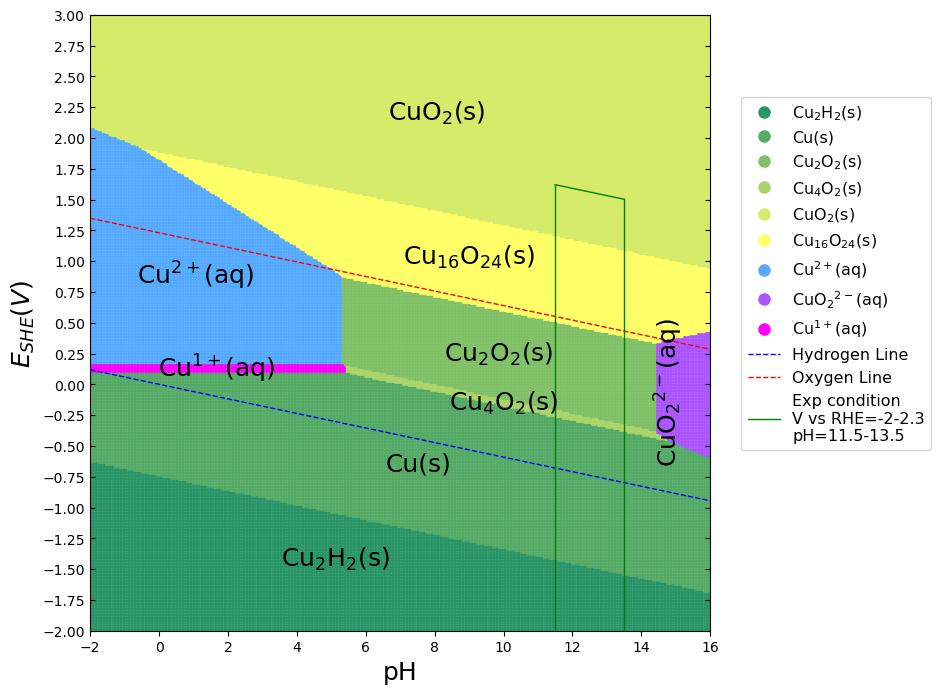
\includegraphics[width=\textwidth]{Figures/pourbaix_diagrams/Cu-NH3-H2O_activity=1e-04_[NH3]=0M_[Gly]=0M_[CN]=0.png}
       % \par\medskip
    \end{subfigure}
    \begin{subfigure}[b]{0.3\textwidth}
        \subcaption{}\label{fig:Cu_Pourbaix_NH3_Gly}
        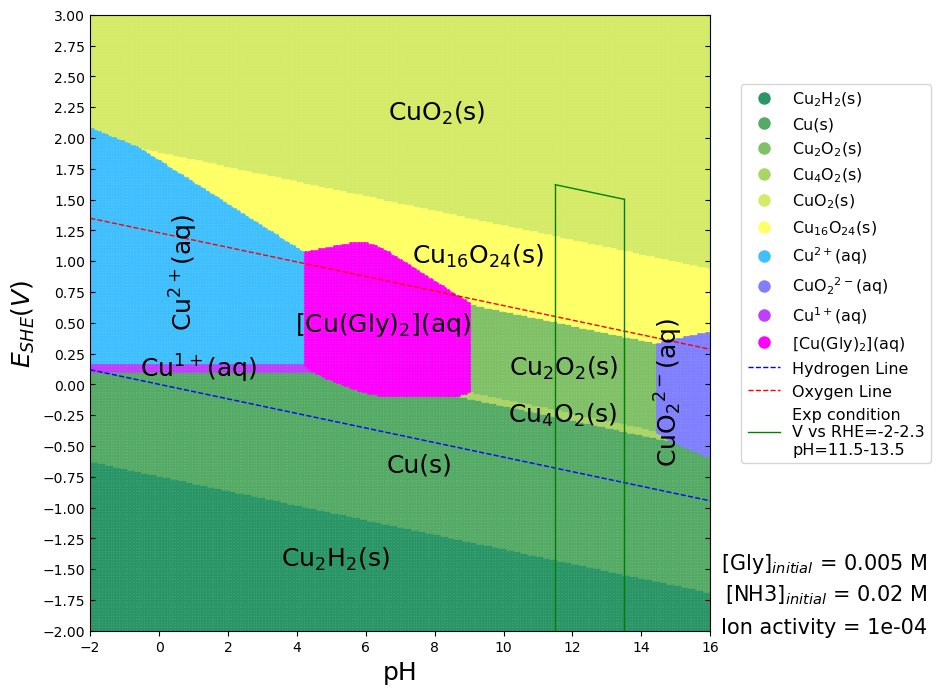
\includegraphics[width=\textwidth]{Figures/pourbaix_diagrams/Cu-NH3-H2O_activity=1e-04_[NH3]=0.02M_[Gly]=0.005M_[CN]=0.png}
       % \par\medskip
    \end{subfigure}
    \begin{subfigure}[b]{0.3\textwidth}
        \subcaption{}\label{fig:Cu_Pourbaix_NH3_Gly_CN}
        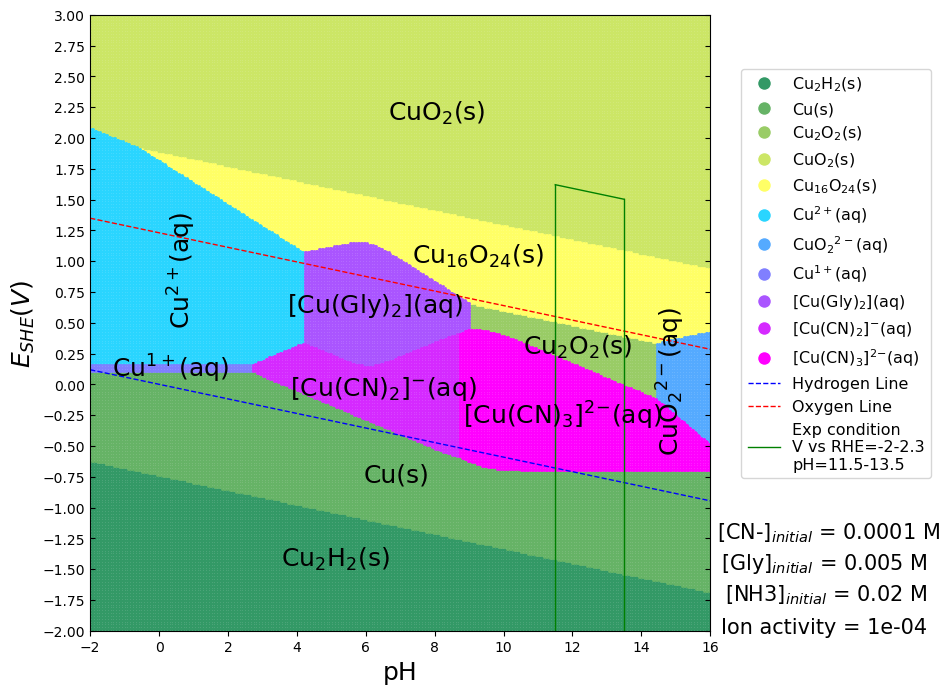
\includegraphics[width=\textwidth]{Figures/pourbaix_diagrams/Cu-NH3-H2O_activity=1e-04_[NH3]=0.02M_[Gly]=0.005M_[CN]=0.0001.png}
       % \par\medskip   
    \end{subfigure}
    \caption{Cu Pourbaix diagrams, with $\text{ion activity}=\num{1e-4}$, (a)\ce{H2O} only, (b)$[\ce{NH3}]_{initial}= 0.02$M, $[\text{Gly}]_{initial}=0.005$M, (c)$[\ce{NH3}]_{initial}= 0.02$M, $[\text{Gly}]_{initial}=0.005$M,  $[\ce{CN-}]_{initial}=\num{1e-4}$M. The green box indicates the experimental condition at applied potential vs RHE = -2 to 2V, pH = 11.5 to 13.5.}
    \label{fig:Cu_Pourbaix}
\end{figure}

\subsubsection{Gold (Au) Stability and Corrosion Behavior}
Gold-based materials have emerged as a promising class of electrocatalysts toward nitrogen reduction reaction with low overpotentials \cite{Ma2021ElectroreductionGold, Shi2017AuConditions, Lee2025FavoringApproach, Bao2017ElectrochemicalCycle}. In the context of EWAS, Au has also demonstrated activity toward glycine oxidation \cite{Sandoval2011AdsorptionStudy, Chen2013AdsorptionStudy, Zou1999GoldIII-inducedGlycine} and oxidation of hydrocarbons \cite{Pina2012UpdateGold, Hughes2005TunableConditions, Scire2012SupportedCompounds}. Au-based heterogeneous catalysts also exhibit resistance to oxidation and corrosion \cite{Gong2009SurfaceGold}. These properties motivate a closer examination of its thermodynamic stability under EWAS-relevant conditions.

\Cref{fig:Au_Pourbaix_NH3_Gly} shows the Pourbaix diagram for Au in the presence of \ce{NH3} and glycine at concentrations of 0.02M and 0.005~M, respectively. Gold readily forms the \ce{[Au(NH3)_2]^+} complex, which is thermodynamically stable over a wide pH range (4.5–14), indicating its susceptibility to leaching in ammoniacal solutions. Although glycine does not form stable Au complexes in the thermodynamic predictions, amino acids, including glycine, have been reported to complex with dissolved gold species at much higher concentrations in prior experimental studies \cite{Sarvar2023ApplicationStructure, Brown1982TheGold}. Therefore, glycine-induced complexation might become more relevant under concentrated or kinetically favorable conditions.

Furthermore, as shown in \Cref{fig:Au_Pourbaix_NH3_Gly_CN}, Au dissolution can be caused by formation of the highly stable \ce{[Au(CN)_2]^-} complex, at low cyanide concentrations (\num{1e-4}~M). The dissolution behavior is consistent with the historical use of cyanide in gold leaching for ore processing due to its high efficiency and low cost \cite{Hilson2006AlternativesFuture, young2001cyanide}.

%%%%%%%%%%%%%%%%%%%%%%%%%%%%%%%%% Au %%%%%%%%%%%%%%%%%%%%%%%%%%%%%%%%%
\begin{figure}[htbp]
    \centering
    \begin{subfigure}[b]{0.3\textwidth}
        \subcaption{}\label{fig:Au_Pourbaix_H2O}
        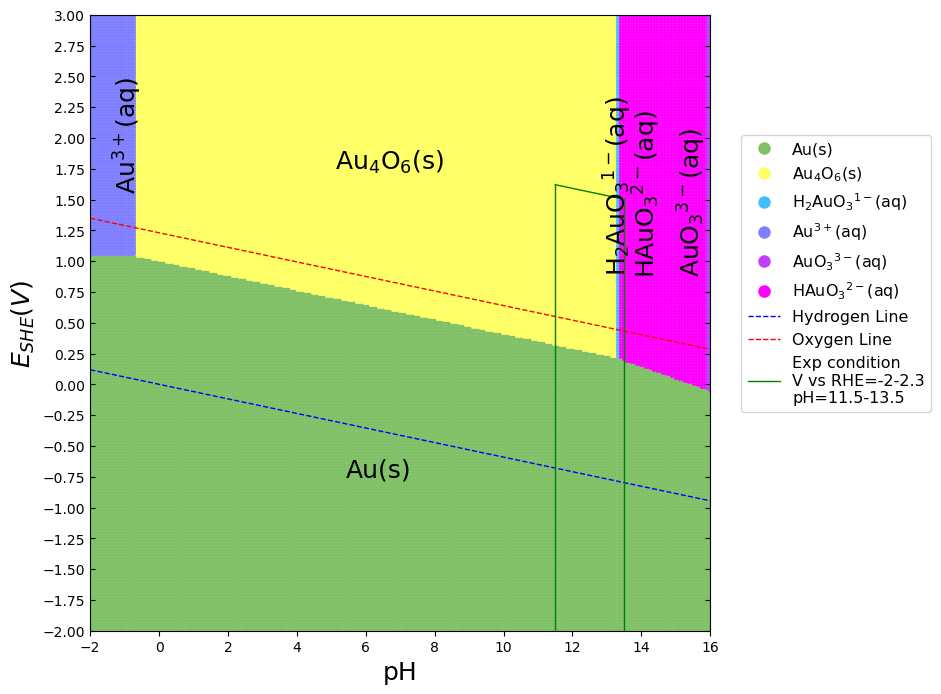
\includegraphics[width=\textwidth]{Figures/pourbaix_diagrams/Au-NH3-H2O_activity=1e-04_[NH3]=0M_[Gly]=0M_[CN]=0.png}
       % \par\medskip
    \end{subfigure}
    \begin{subfigure}[b]{0.3\textwidth}
        \subcaption{}\label{fig:Au_Pourbaix_NH3_Gly}
        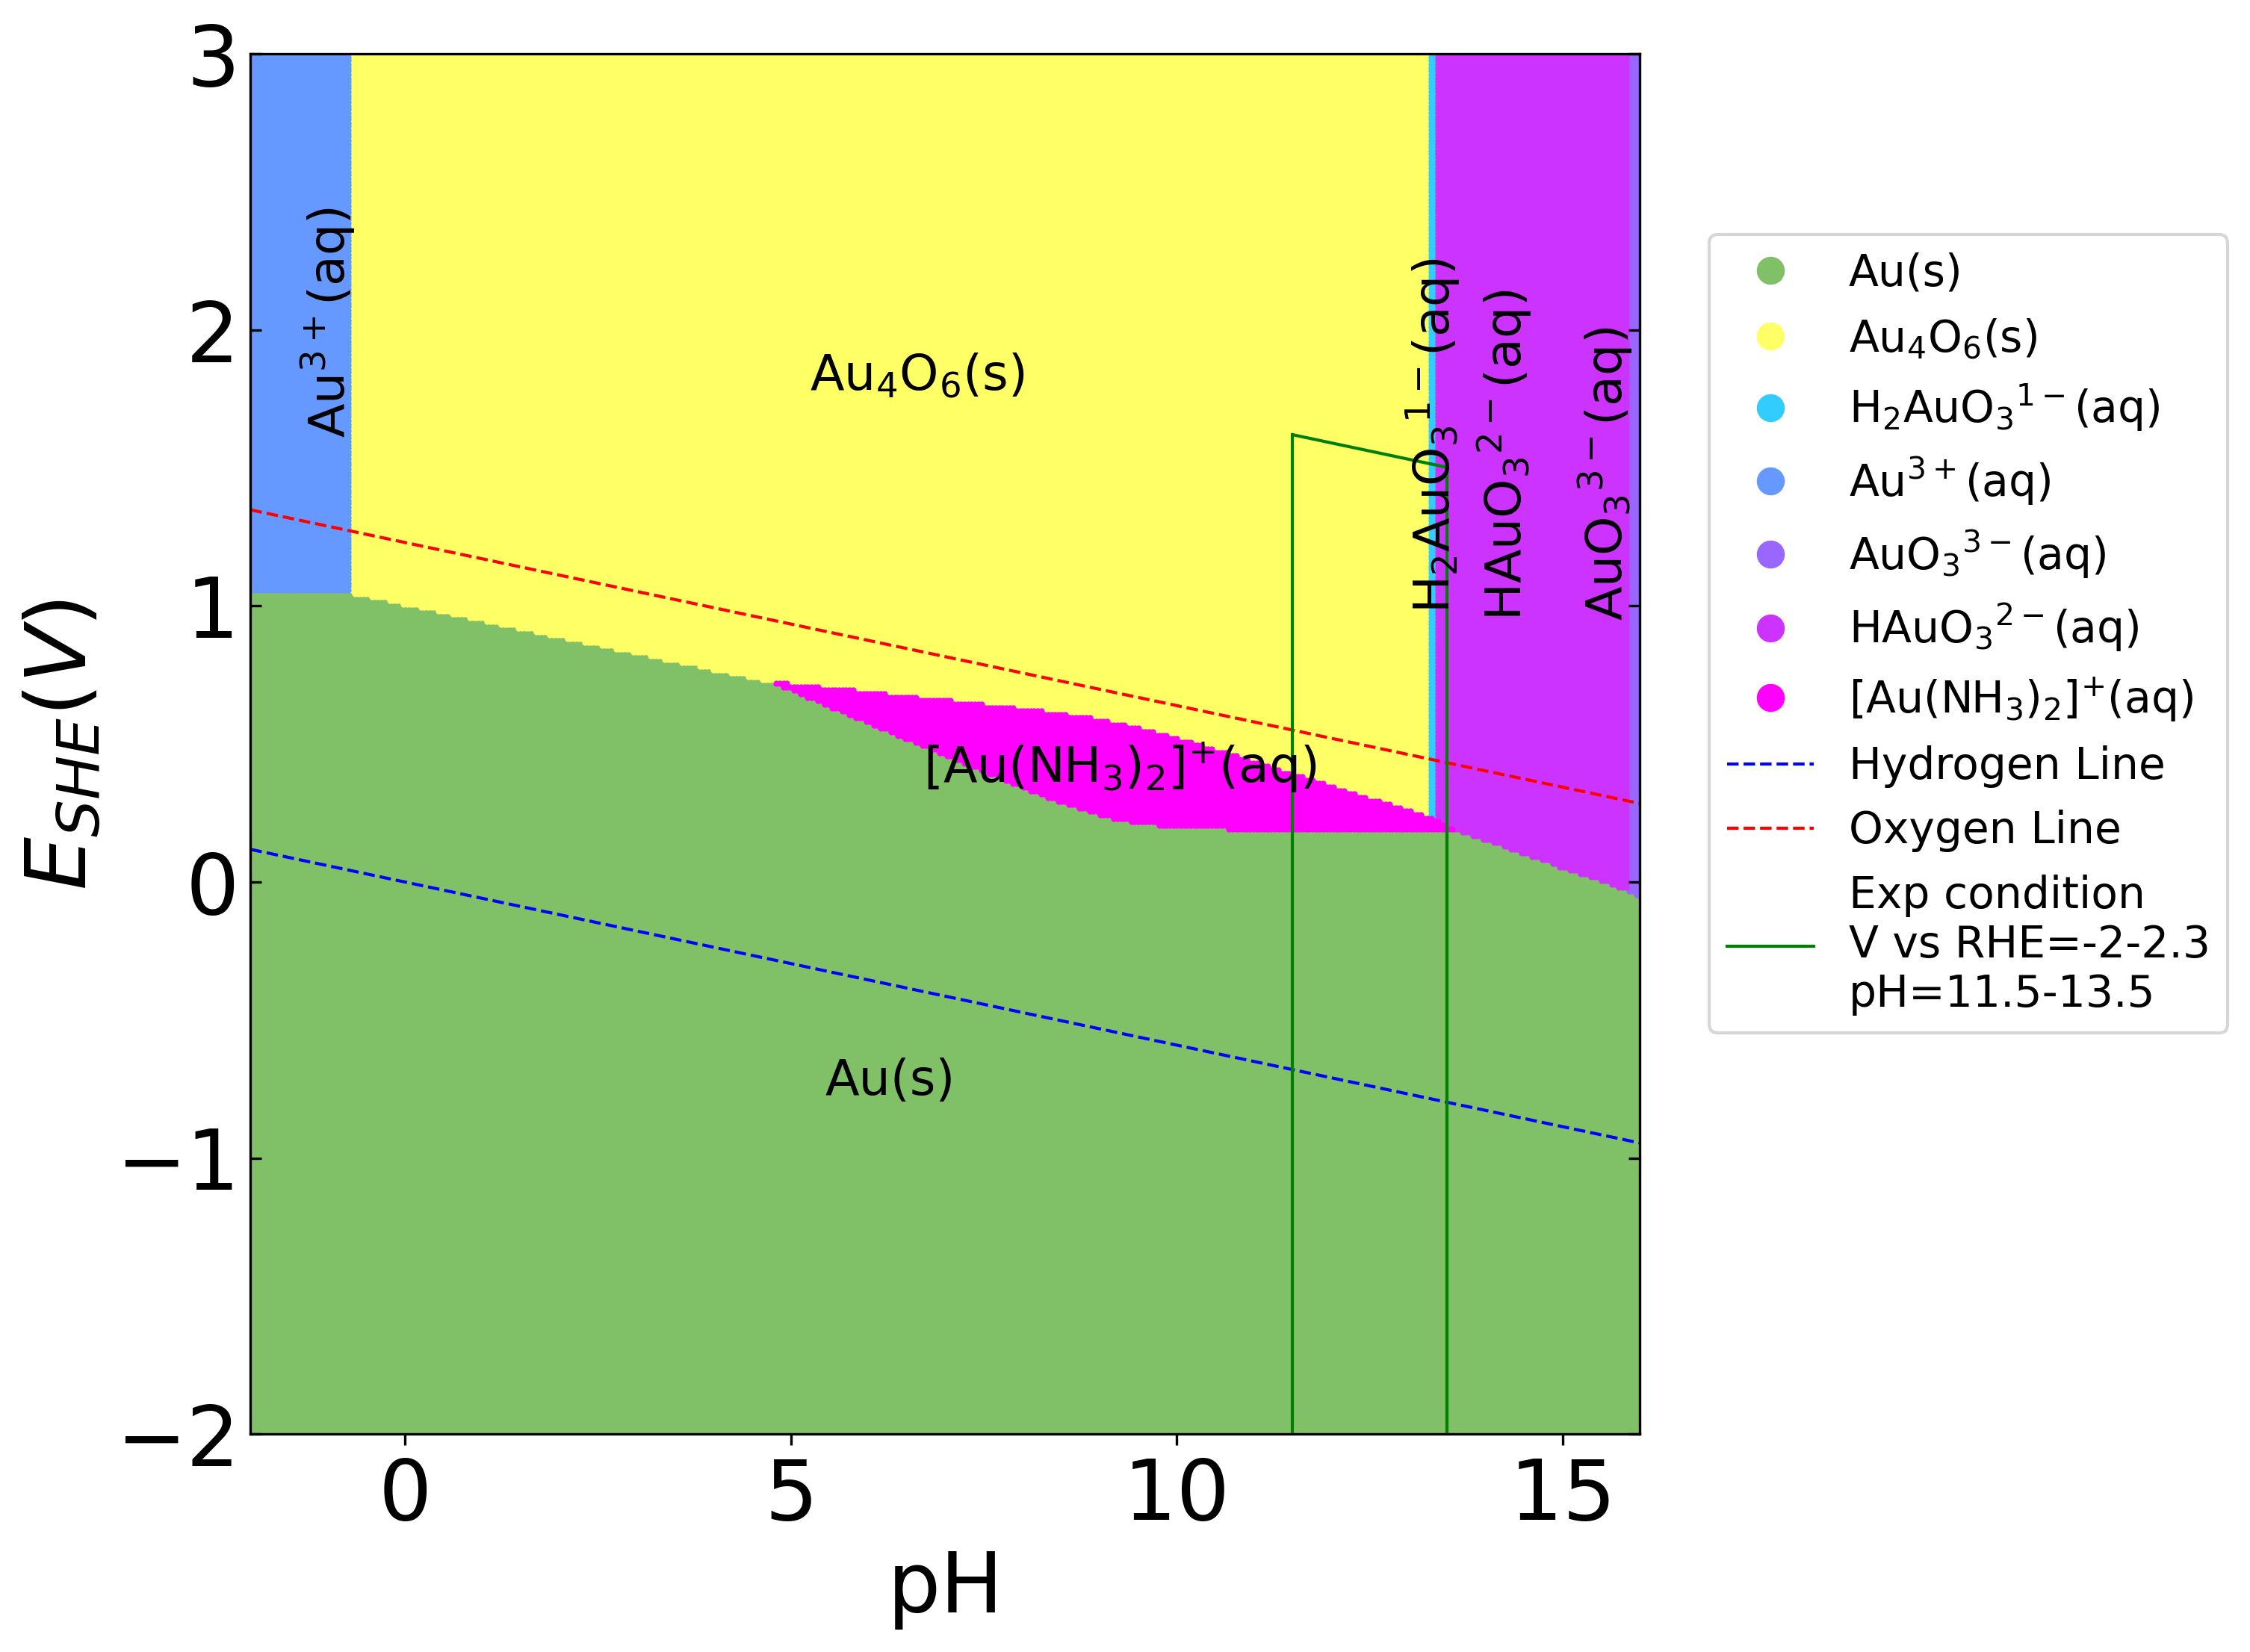
\includegraphics[width=\textwidth]{Figures/pourbaix_diagrams/Au-NH3-H2O_activity=1e-04_[NH3]=0.02M_[Gly]=0.005M_[CN]=0.png}
       % \par\medskip
    \end{subfigure}
    \begin{subfigure}[b]{0.3\textwidth}
        \subcaption{}\label{fig:Au_Pourbaix_NH3_Gly_CN}
        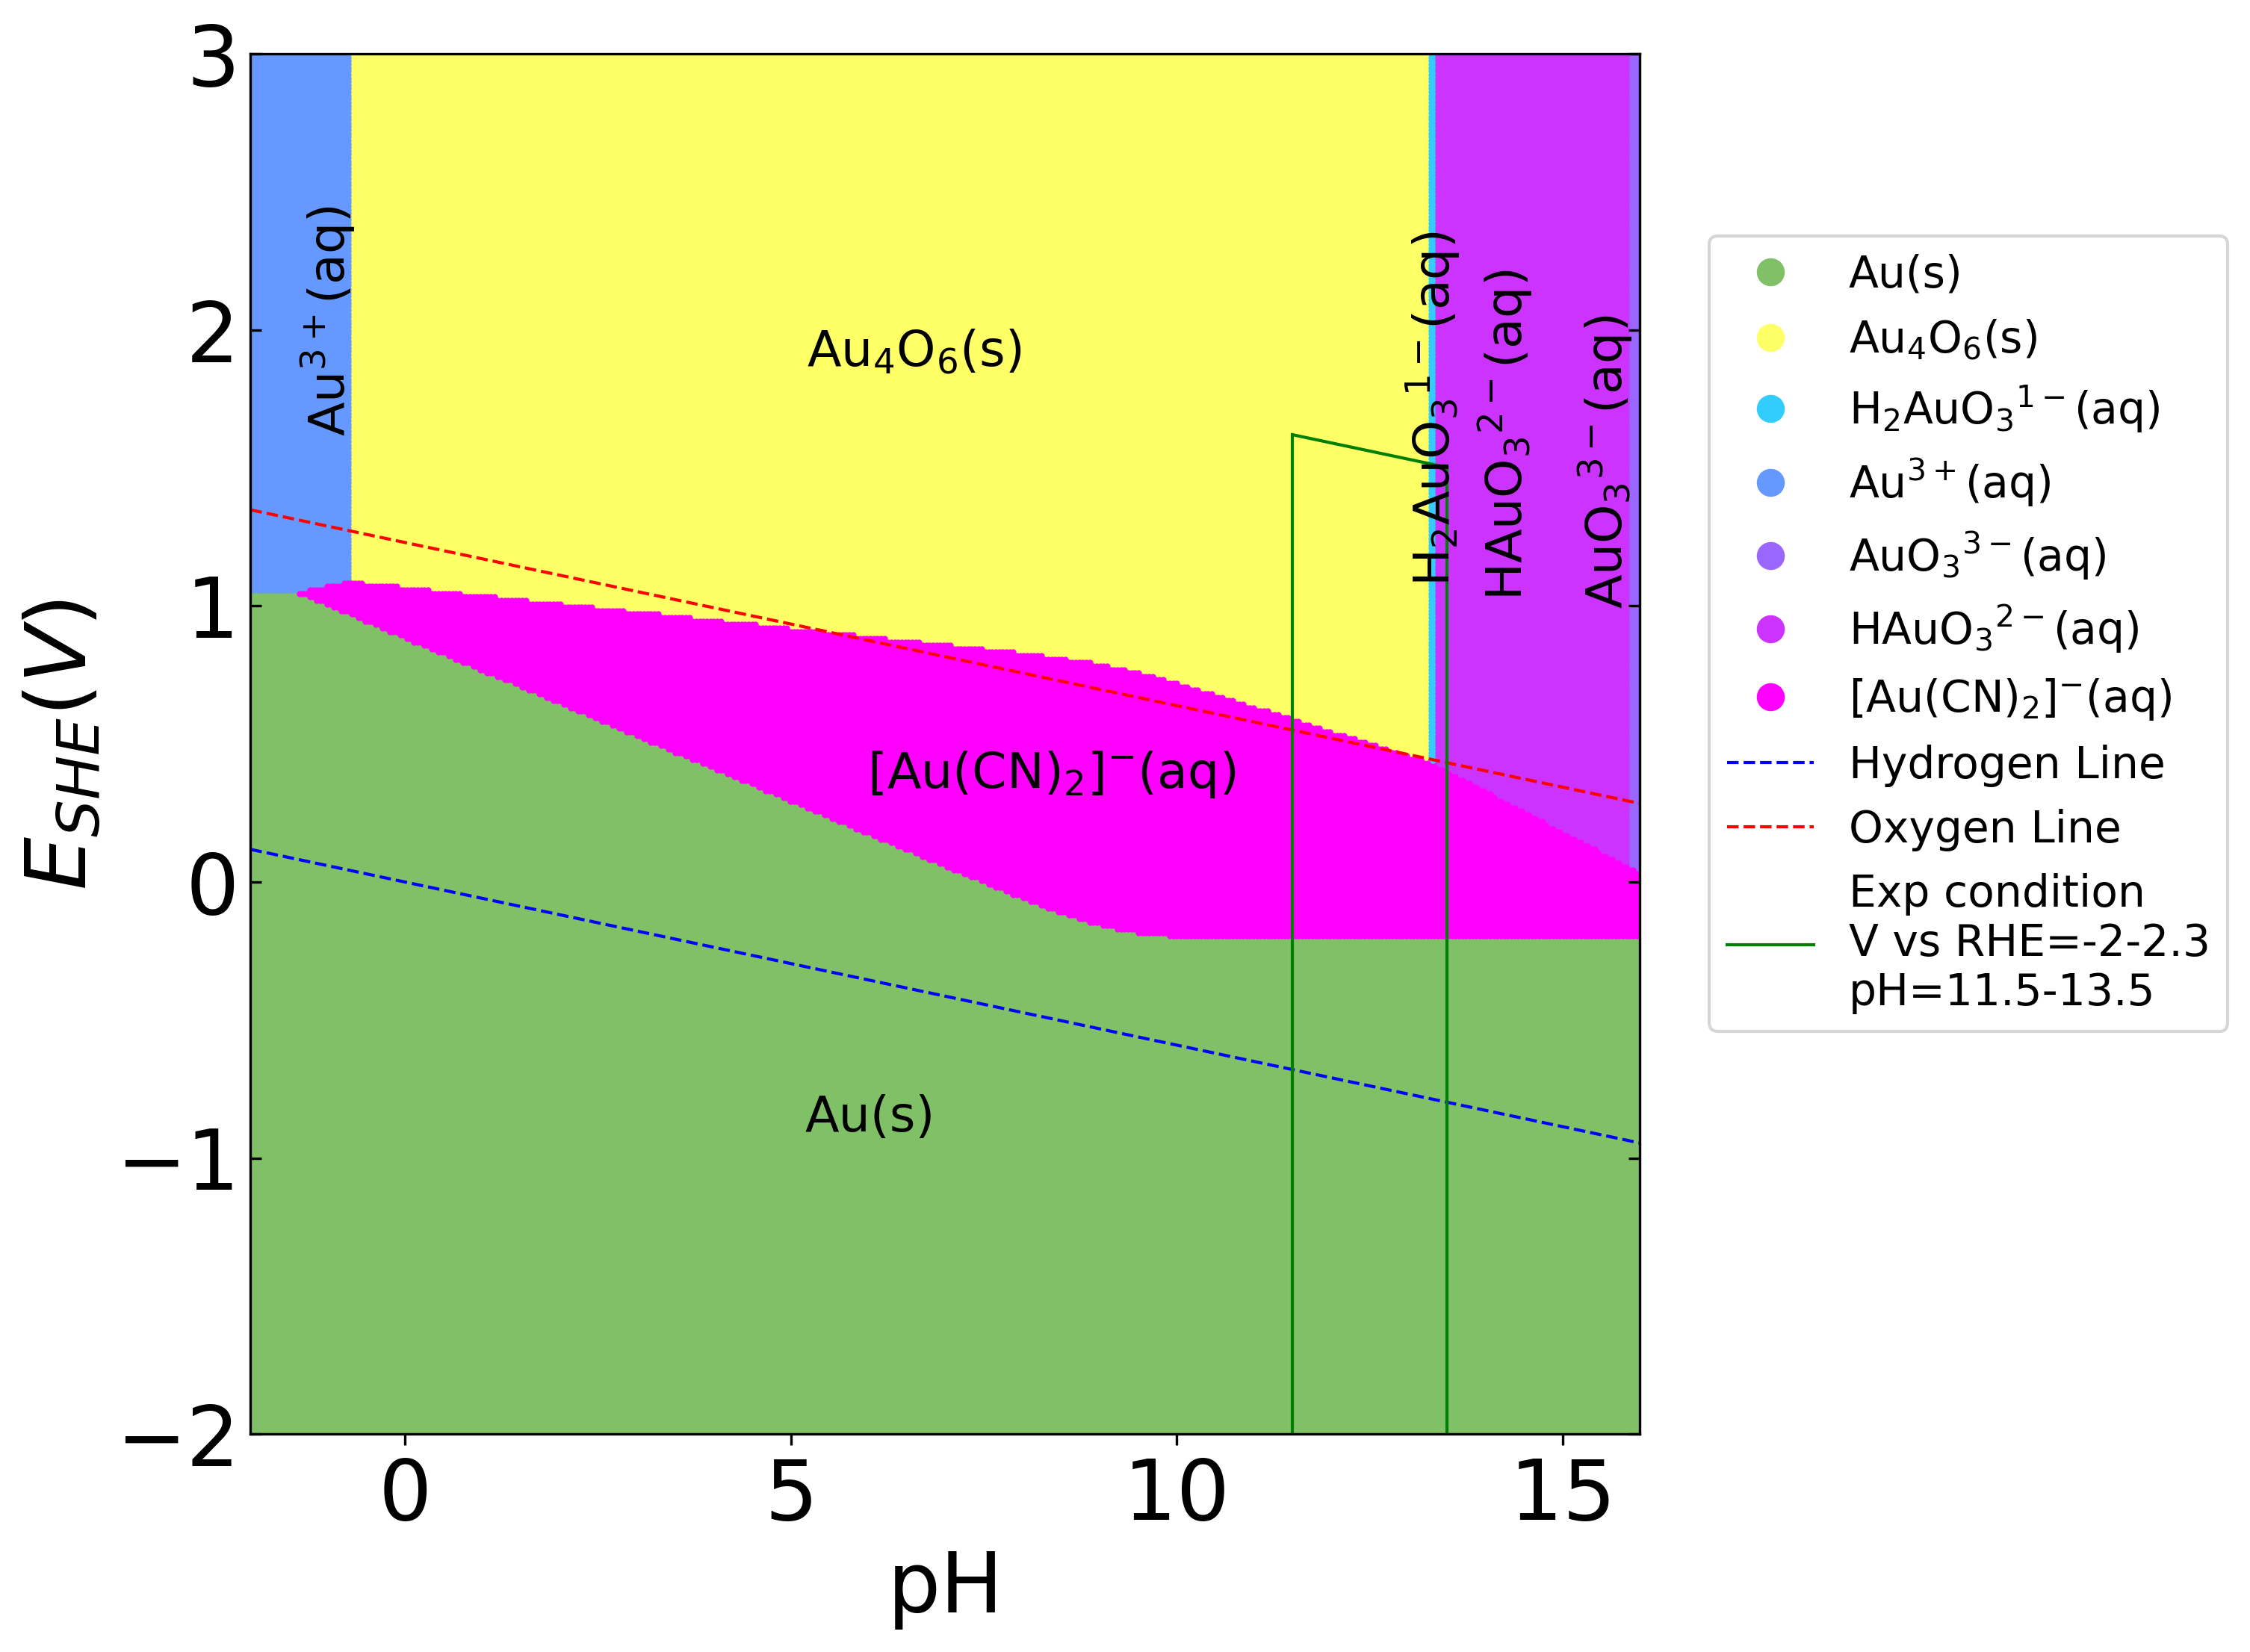
\includegraphics[width=\textwidth]{Figures/pourbaix_diagrams/Au-NH3-H2O_activity=1e-04_[NH3]=0.02M_[Gly]=0.005M_[CN]=0.0001.png}
       % \par\medskip   
    \end{subfigure}
    \caption{Au Pourbaix diagrams, with $\text{ion activity}=\num{1e-4}$, (a)\ce{H2O} only, (b)$[\ce{NH3}]_{initial}= 0.02$M, $[\text{Gly}]_{initial}=0.005$M, (c)$[\ce{NH3}]_{initial}= 0.02$M, $[\text{Gly}]_{initial}=0.005$M,  $[\ce{CN-}]_{initial}=\num{1e-4}$M. The green box indicates the experimental condition at applied potential vs RHE = -2 to 2V, pH = 11.5 to 13.5.}
    \label{fig:Au_Pourbaix}
\end{figure}

\subsubsection{Palladium (Pd) Stability and Cyanide Complex Formation} 

Like other platinum-group metals, palladium exhibits high catalytic activity in a variety of electrochemical processes, including the hydrogen evolution reaction,  glycine decomposition, and reduction of simple organic compounds \cite{Grden2008ElectrochemicalAdsorption, Baldauf1996FormicElectrodes, Simonet2005TheRadicals, ukaszewski2003ElectrosorptionAlloys, Jiang2021SpectrometricElectrodes, Rugira2025ExperimentalHydrodechlorination, Gao2007ChemistryStudy, Burke1993AnAcid}.

As shown in \Cref{fig:Pd_Pourbaix}, Pd remains thermodynamically stable across the EWAS-relevant pH and potential range when exposed to \ce{NH3} and glycine. While Pd can form glycine complexes such as \ce{[Pd(Gly)^+]} and \ce{[Pd(Gly)_2]}, these complexes have relatively low stability constants and do not significantly alter Pd's passivation behavior. However, the introduction of cyanide dramatically reduces Pd’s stability. Even at low \ce{CN^-} concentrations (e.g., \num{1e-4}~M), the highly stable \ce{[Pd(CN)_4]^{2-}} complex dominates the Pourbaix diagram, significantly expanding the corrosion region (\Cref{fig:Pd_Pourbaix_NH3_Gly_CN}).

Notably, reported stability constants for \ce{[Pd(CN)_4]^{2-}} vary considerably in the literature, ranging from $log\beta_4 = 42.2$ \cite{Smith1989CriticalConstants} to as high as $log\beta_4 = 63$ \cite{Cabbiness1969MacrocyclicComplexes}. The Pourbaix diagram in \ref{fig:Pd_Pourbaix_NH3_Gly_CN} is based on an updated stability constant of $log\beta_4 = 62.3$, as determined by Harrington et al. \cite{Harrington2005DeterminationIon}. Harrington’s study suggests that earlier stability constant values, such as $log\beta_4 = 42.4$ reported by Smith et al. \cite{Smith1989CriticalConstants}, were inaccurate due to incorrect electrochemical potential measurements. 

% Given these uncertainties and the high cost of Pd electrodes, avoiding conditions that promote \ce{[Pd(CN)4^2+]} formation is advisable.

%%%%%%%%%%%%%%%%%%%%%%%%%%%%%%%%% Pd %%%%%%%%%%%%%%%%%%%%%%%%%%%%%%%%%
\begin{figure}[htbp]
    \centering
    \begin{subfigure}[b]{0.45\textwidth}
        \subcaption{}\label{fig:Pd_Pourbaix_NH3_Gly}
        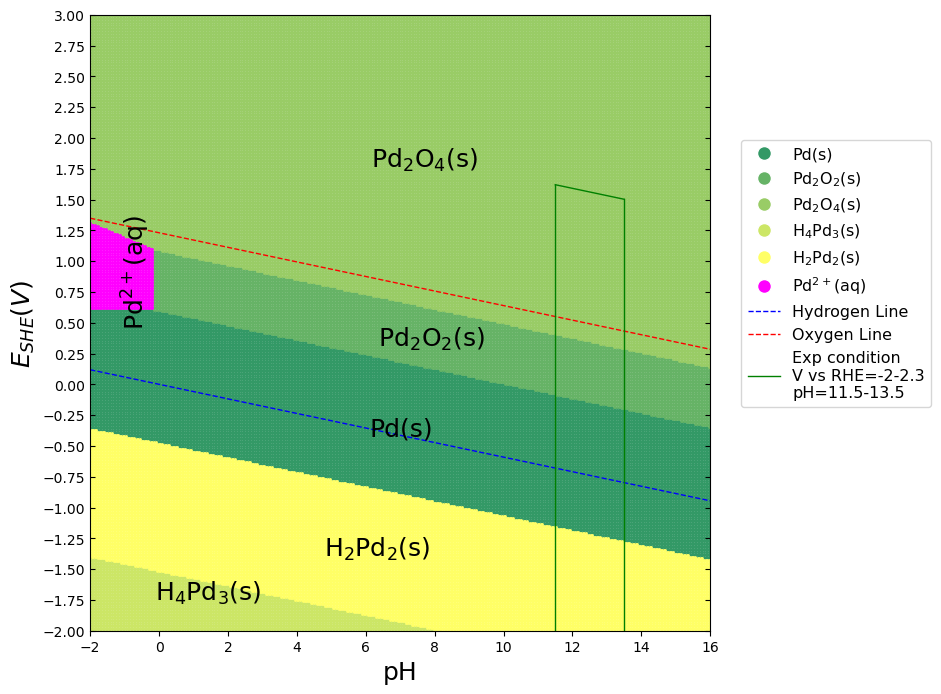
\includegraphics[width=\textwidth]{Figures/pourbaix_diagrams/Pd-NH3-H2O_activity=1e-04_[NH3]=0.02M_[Gly]=0.005M_[CN]=0.png}
       % \par\medskip
    \end{subfigure}
    \begin{subfigure}[b]{0.45\textwidth}
        \subcaption{}\label{fig:Pd_Pourbaix_NH3_Gly_CN}
        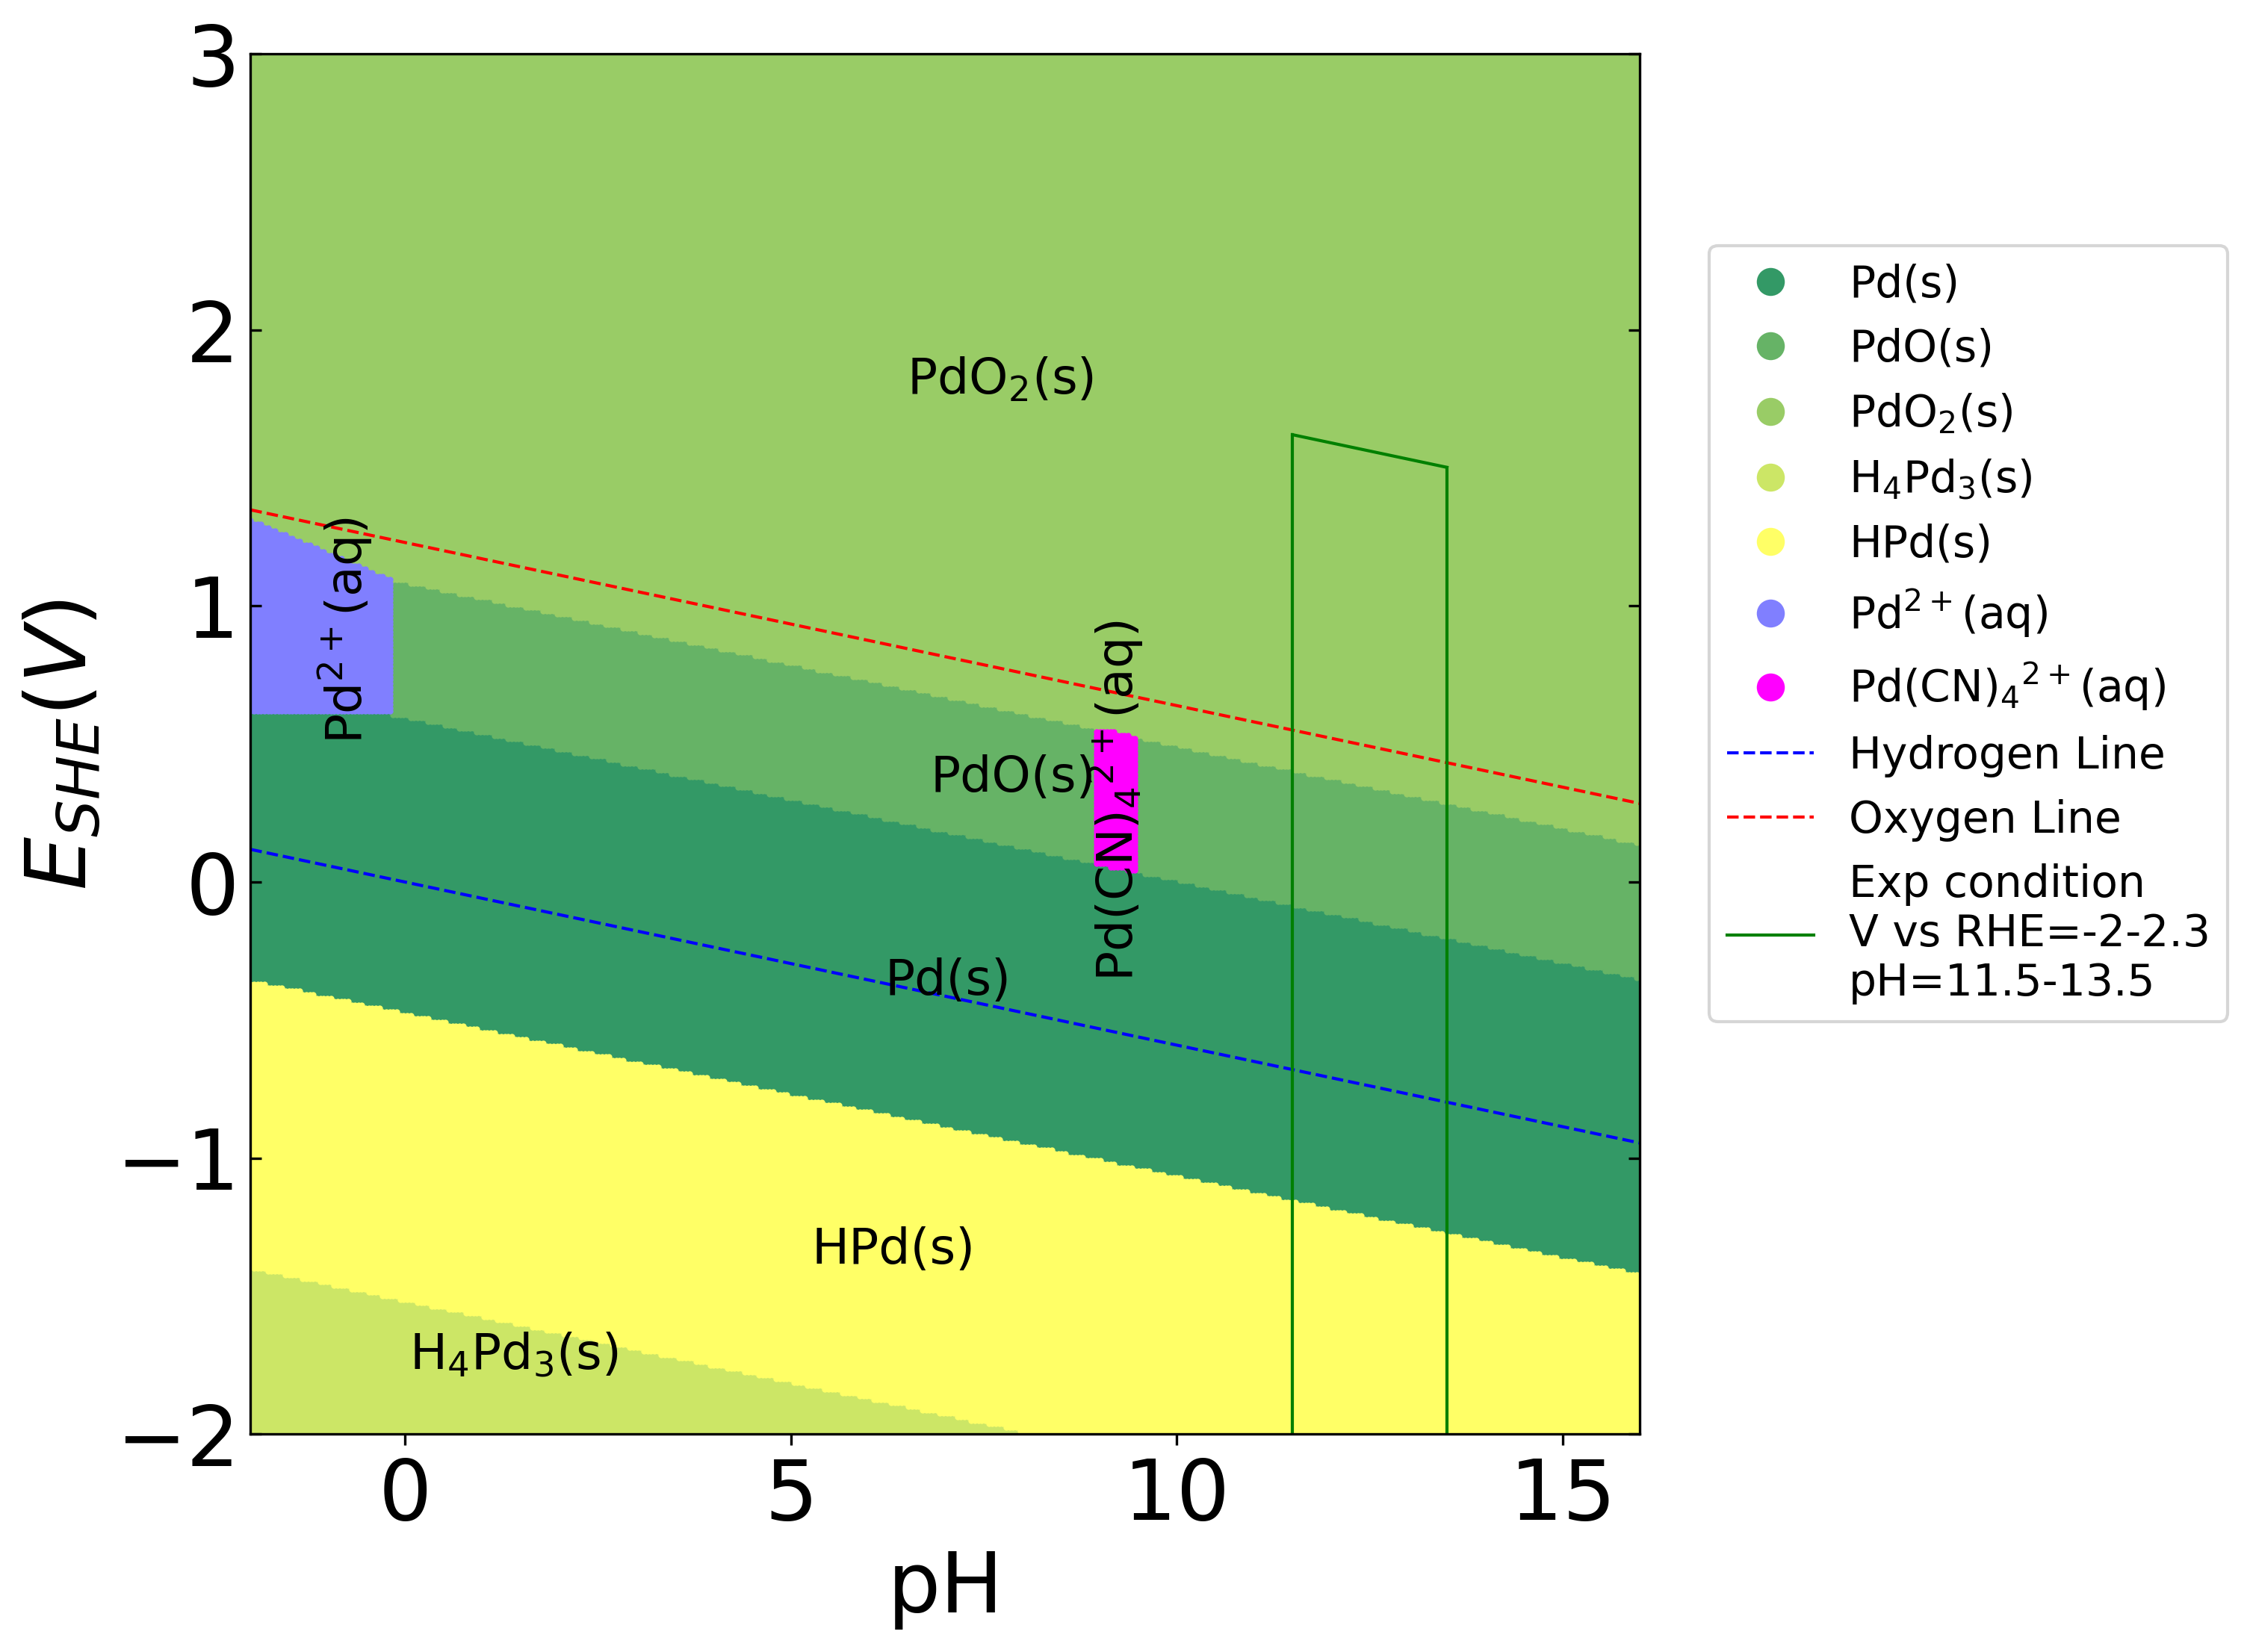
\includegraphics[width=\textwidth]{Figures/pourbaix_diagrams/Pd-NH3-H2O_activity=1e-04_[NH3]=0.02M_[Gly]=0.005M_[CN]=0.0001.png}
       % \par\medskip   
    \end{subfigure}

    \caption{Pd Pourbaix diagrams, with $\text{ion activity}=\num{1e-4}$, (a)$[\ce{NH3}]_{initial}= 0.02$M, $[\text{Gly}]_{initial}=0.005$M, (b)$[\ce{NH3}]_{initial}= 0.02$M, $[\text{Gly}]_{initial}=0.005$M,  $[\ce{CN-}]_{initial}=\num{1e-4}$M. Green box indicates experimental condition at applied potential vs RHE = -2 to 2V, pH = 11.5 to 13.5.}
    \label{fig:Pd_Pourbaix}
\end{figure}


\subsubsection{Platinum (Pt) Stability and Cyanide Complexation}

Platinum is known for its exceptional catalytic properties \cite{Debe2012ElectrocatalystCells, Daubinger2014ElectrochemicalStudy} in the oxygen reduction and hydrogen oxidation reaction in fuel cells. It exhibits excellent chemical and physical characteristics, including high electrical conductivity, good ductility, and electrocatalytic activity toward a wide range of anodic and cathodic electrochemical reactions \cite{Jerkiewicz2022ApplicabilityResearch}. Numerous studies, some dating back to the early 1970s, have reported the (electro)dissolution behavior of Pt in acidic and alkaline aqueous electrolytes \cite{Rand1972AVoltammetry, Tian2016InfluenceConditions, Xing2014PlatinumCycling}. However, reports specifically addressing Pt dissolution in the presence of glycine or ammonia are limited.

The Pourbaix diagram for Pt in the presence of \ce{NH3}, glycine and \ce{CN^-} ligands is shown in \Cref{fig:Pt_Pourbaix_NH3_Gly_CN}. No reliable stability constants for \ce{Pt^2+}-glycine complexes have been reported, as noted by Kiss et al. \cite{Kiss1991CriticalGlycine}. Its complexation with cyanide is better characterized. The square-planar, diamagnetic \ce{[Pt(CN)_4]^{2-}} complex is known to be highly stable \cite{Griffith1962CyanideMetals}, with a commonly cited $log\beta_4$ of 41 \cite{Smith1989CriticalConstants}. However, this value is debatable, as it was determined under non-equilibrium conditions. More recent spectrophotometric studies \cite{Hancock1976FormationTetrakiscyanopalladate2-} suggest significantly higher values, likely in the range of $log\beta_4$ 65–75. Using an estimated $log\beta_4 = 70$, the Pourbaix diagram (see \Cref{fig:Pd_Pourbaix_Smith1989CriticalConstants_SI}) reveals that \ce{[Pt(CN)_4]^{2-}} is the thermodynamically favored species across a broad pH window that overlaps with the EWAS-relevant pulsing potential range (–2 to 2 V). 

\subsubsection{Titanium (Ti) Stability and Suitability for EWAS}

The Pourbaix diagram for Ti in aqueous solution with glycine ligands is shown in \ref{fig:Ti_Pourbaix_NH3_Gly_CN}. No stable \ce{Ti^2+}-\ce{NH3} or \ce{Ti^2+}-\ce{CN^-} complexes have been reported \cite{Griffith1962CyanideMetals, Nicholls1980ComplexTitanium}. The diagram includes the stability constants of \ce{[Ti(Gly)^-]} and \ce{[Ti(Gly)_2^+]}, but glycine concentration does not significantly impact Ti's passivity over the targeted potential and pH range. Due to its ability to form a stable passive oxide layer \cite{Kiss1991CriticalGlycine, PourbaixAtlasSolutions}, Ti is highly dissolution-resistant, with limited experimental evidence of dissolution \cite{Schmidt2009AqueousVoltammetry, Ziemniak1993SolubilityTemperatures, Knauss2001TiIV300C, Schmidt2006DissolutionEffect, Pocsi1988ComplexAcid}.

Despite its excellent thermodynamic stability, a key limitation of Ti-based materials is the low electronic conductivity of their passive oxide layer. The wide band gap of \ce{TiO2} hinders efficient electron transport and can affect catalytic performance in electrochemical systems. Modifications such as MXenes \cite{Gardon2013ImprovedSpray, Naguib2012Two-DimensionalCarbides, Hui2022VacancyBatteries} and doped perovskites like \ce{SrTiO3} \cite{Sokolov2024ComputationalTitanate} can improve conductivity. While their thermodynamic stability is an advantage, the viability of Ti-based electrodes in EWAS systems will ultimately depend on strategies to overcome these conductivity limitations.
% Thus, Ti-based materials can be promising candidates for EWAS electrodes due to their corrosion resistance and potential for electronic conductivity enhancement.

%%%%%%%%%%%%%%%%%%%%%%%%%%%%%%%%% Pt and Ti %%%%%%%%%%%%%%%%%%%%%%%%%%%%%%%%%
\begin{figure}[htbp]
    \centering
    \begin{subfigure}[b]{0.45\textwidth}
        \subcaption{}\label{fig:Ti_Pourbaix_NH3_Gly_CN}
        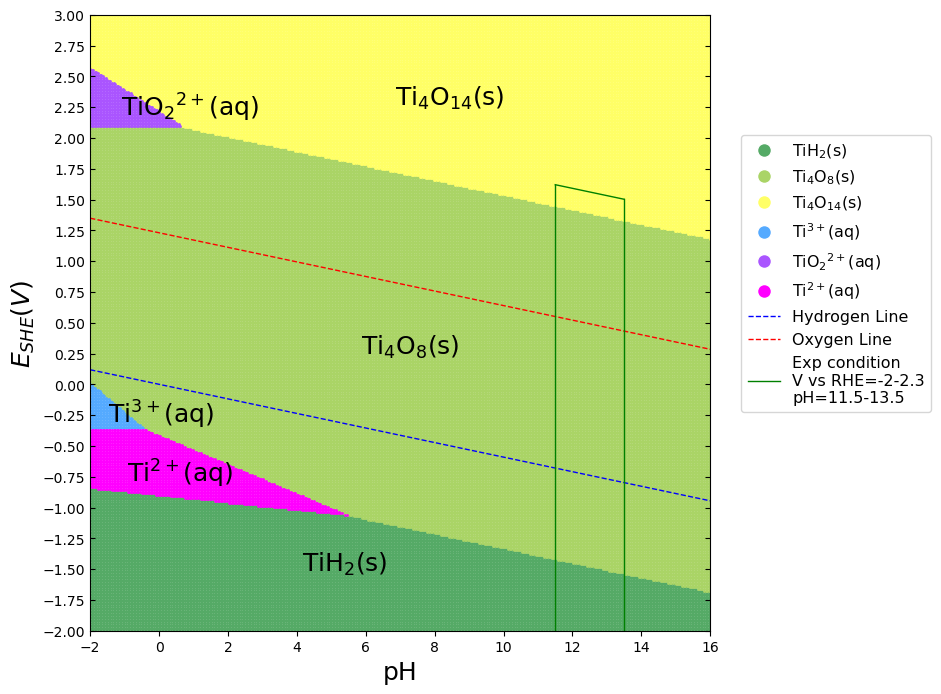
\includegraphics[width=\textwidth]{Figures/pourbaix_diagrams/Ti-NH3-H2O_activity=1e-04_[NH3]=0.02M_[Gly]=0.005M_[CN]=0.0001.png}
       % \par\medskip
    \end{subfigure}
    \begin{subfigure}[b]{0.45\textwidth}
        \subcaption{}\label{fig:Pt_Pourbaix_NH3_Gly_CN}
        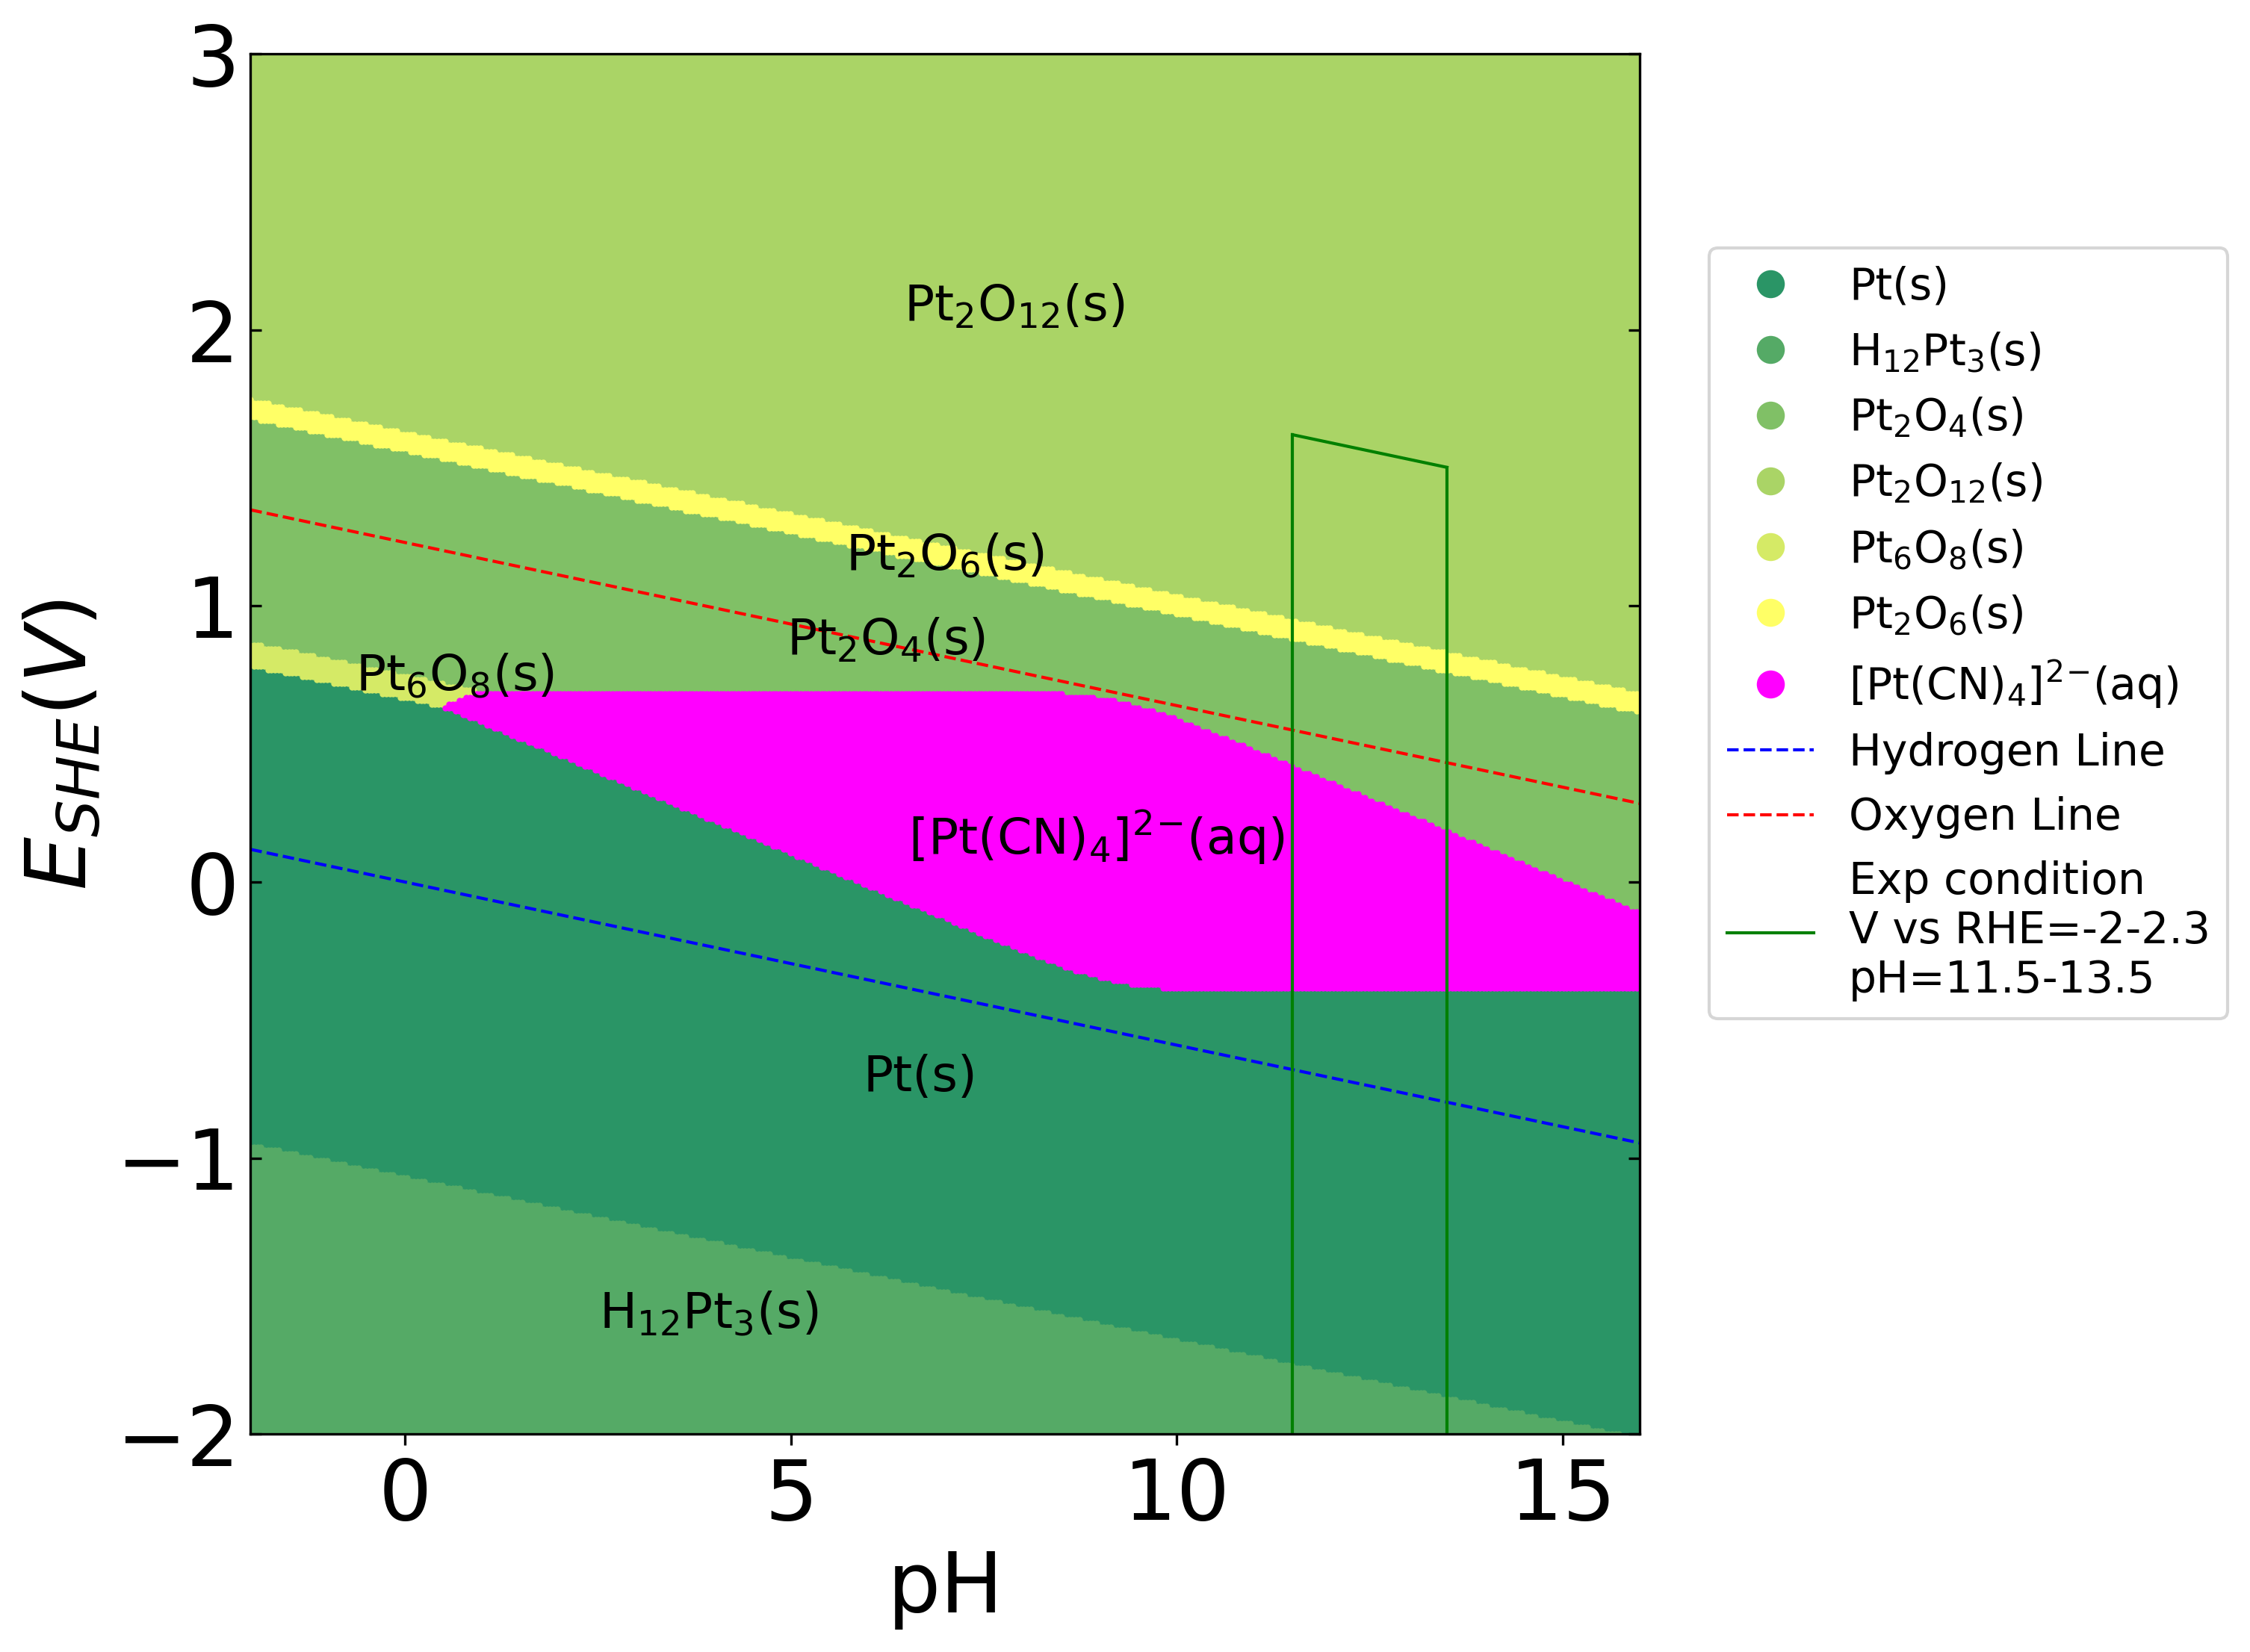
\includegraphics[width=\textwidth]{Figures/pourbaix_diagrams/Pt-NH3-H2O_activity=1e-04_[NH3]=0.02M_[Gly]=0.005M_[CN]=0.0001.png}
       % \par\medskip   
    \end{subfigure}
    \caption{Pourbaix diagrams of (a) Ti, (b) Pt. $\text{Ion activity}=\num{1e-4}$, $[\ce{NH3}]_{initial}= 0.02$M, $[\text{Gly}]_{initial}=0.005$M,  $[\ce{CN-}]_{initial}=\num{1e-4}$M. The green box indicates the experimental condition at applied potential vs RHE = -2 to 2V, pH = 11.5 to 13.5.}
    \label{fig:Ti_Pt_Pourbaix}
\end{figure}


\subsection{Thermodynamic screening of alloys} \label{sec:alloy_screening}

To identify materials that enhance both conductivity and electrochemical stability, we extended our thermodynamic screening to binary alloy systems using bulk Pourbaix diagrams. These diagrams provide insight into the thermodynamic stability of alloy phases under EWAS-relevant pH and potential ranges. Among the range of candidate systems, alloys based on Ti and Pd emerged as particularly promising due to the corrosion resistance of the base metals, and the abundance of known stable alloy and alloy-oxide phases reported in the Materials Project database. We examined representative systems, including Ni-Ti and Cu-Ti, Au-Pd and Pt-Pd alloys, to understand how alloying modifies stability in the presence of nitrogen-containing ligands. 




\subsubsection{Ti alloys}

Pourbaix diagrams for Ti-based alloys are shown in \Cref{fig:alloy_pourbaix_collage_1,fig:alloy_pourbaix_collage_2}. These diagrams consider all possible combinations of alloy and oxide species that satisfy the stoichiometric constraints, i.e., metal: Ti = 1:1. A shaded grey region indicates that an alloy or alloy oxide is the dominant contributor to the most thermodynamically stable phase in that region.

Across these diagrams, Ti alloys generally exhibit lower stability at more acidic conditions and may release metal ions such as \ce{Mg^{2+}} and \ce{Mn^{2+}}. Alloys of Ti with Fe, Mn, Ni, and Zn show stable regions within the EWAS-relevant pH and potential window. However, Fe and Mn tend to dissolve under oxidative potentials due to the formation of highly soluble ion species such as \ce{FeO_4^{2-}} and \ce{MnO_4^{-}}. Under highly alkaline conditions (pH $\>$ 13.5), Mg and Sr form stable alloys with Ti; whereas at lower pH, Mg can form stable aqueous glycine complexes, while Sr remains predominantly as \ce{Sr^2+}. 

The Ni-Ti system, including titanium-nickel oxides, exhibits good stability between pH 11 and 12.5 across the entire potential range. At pH $<$ 12, Ni may form glycine complexes, while at pH $>$ 14, it can dissolve as aqueous nickel oxyhydroxide species. The Ti–Zn system forms \ce{Ti3Zn2O8}, which is stable between pH 11 and 13 and coexists with ZnO or \ce{ZnO_2}.

In contrast, Cu–Ti and Au–Ti alloys do not exhibit stable alloy phases in the Pourbaix diagrams; instead, their diagrams primarily reflect overlapping regions from the stability of the respective pure metal oxides and Ti oxides. The abscenc of stable alloys may also stem from systematic errors in DFT calculations, as both Cu–Ti and Au–Ti alloy systems are less extensively studied computationally. Therefore, more accurate thermodynamic data are needed to assess their stability reliably. Notably, Au may still undergo leaching through complexation with \ce{NH3}, forming \ce{[Au(NH3)_2]^+}. In contrast, Cu and its oxide phases appear stable and coexist with Ti oxides across EWAS-relevant pH and potential conditions, making Cu–Ti alloys a promising candidate for further experimental validation.

In the following subsection, we focus on Ni–Ti and Cu–Ti alloys and evaluate their stability under varying concentrations of glycine and cyanide ligands.

%%%%%%%%%%%%%%%%%%%%%%%%%%%%%%%%% Collage of Ti Alloy Pourbaix Diagrams %%%%%%%%%%%%%%%%%%%%%%%%%%%%%%%%%
\begin{figure}[htbp]
\centering
\makebox[\textwidth][c]{%g
        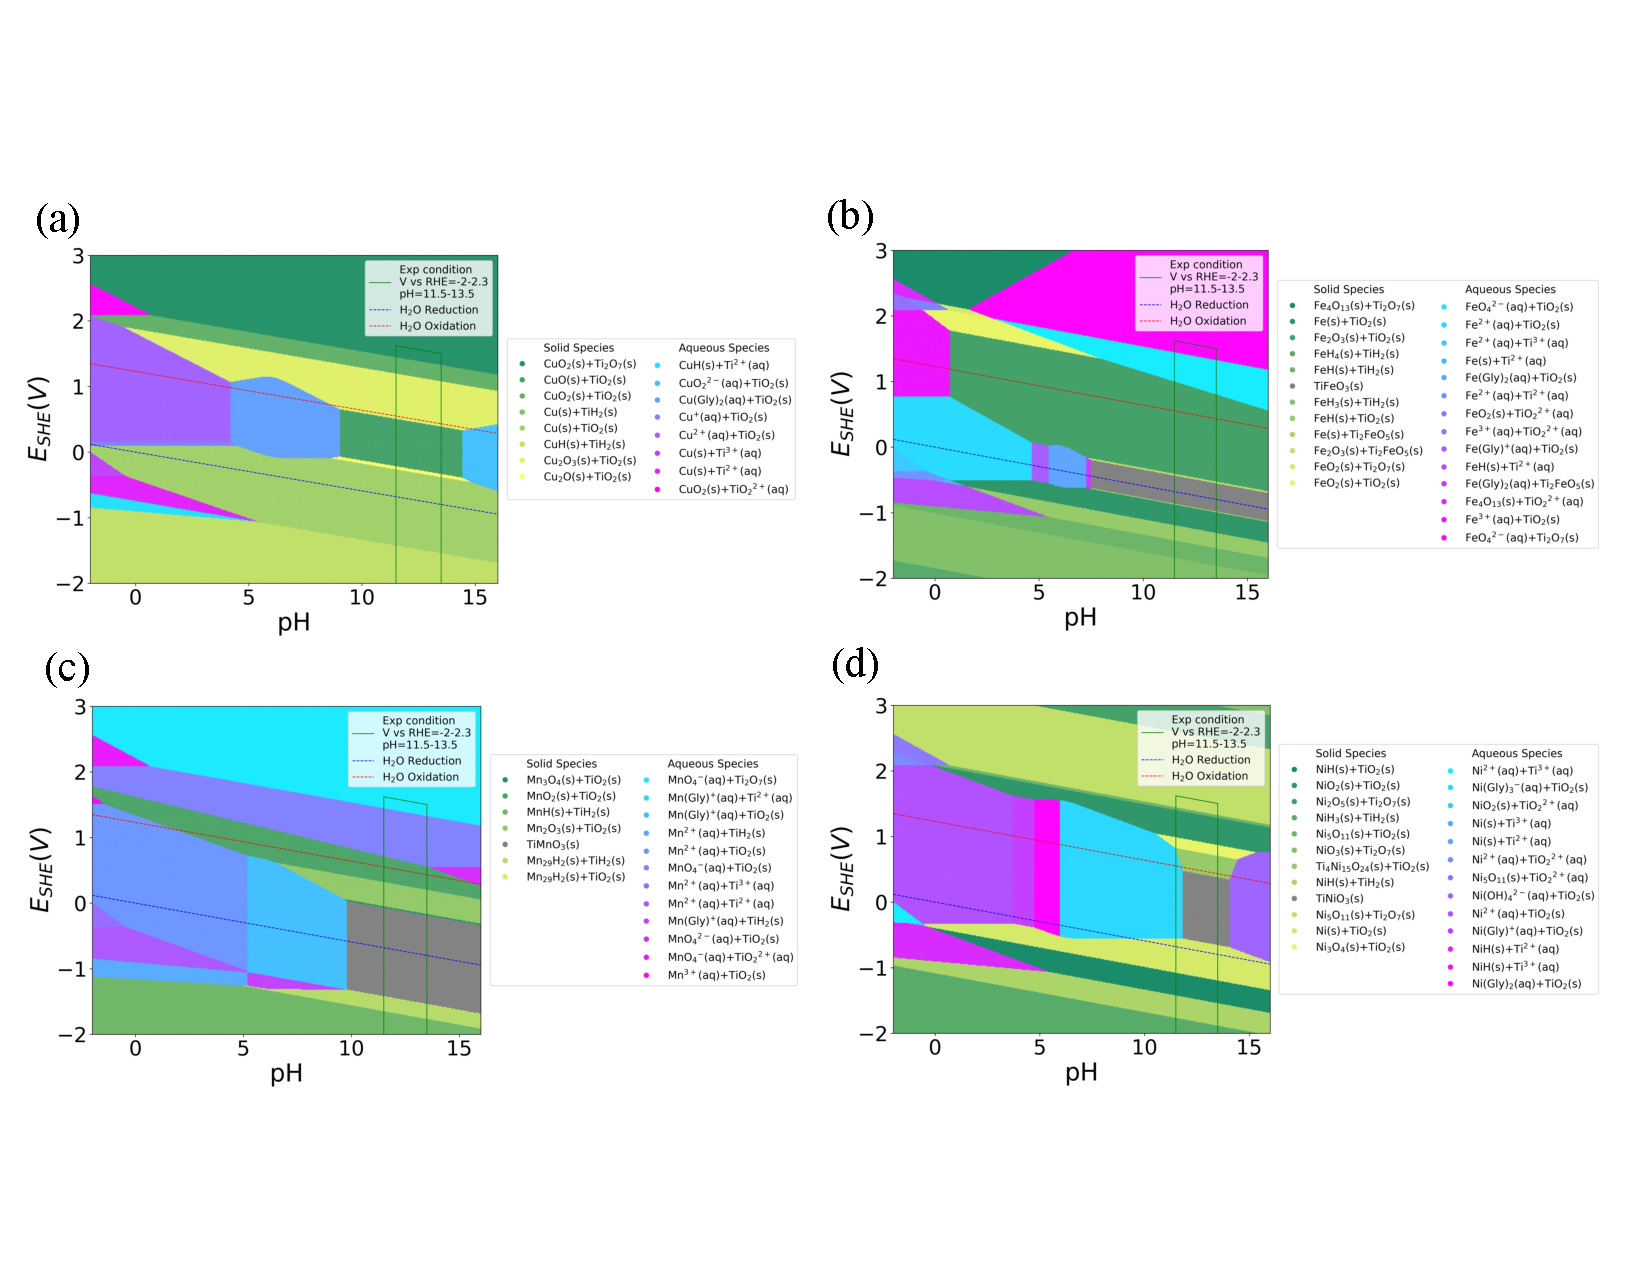
\includegraphics[width=1.1\textwidth]{Figures/alloy_pourbaix_diagrams/alloy_pourbaix_collage_1.pdf}}
\caption{Metal alloy Pourbaix diagrams: (a) Cu-Ti, (b) Fe-Ti, (c) Mn-Ti, (d) Ni-Ti, with $\text{ion activity}=\num{1e-4}$M, $[\ce{NH3}]_{initial}= 0.02$M, $[\text{Gly}]_{initial}=0.005$M. The green box indicates the experimental condition at an applied potential of -2 to 2V vs RHE, pH = 11.5 to 13.5.}
\label{fig:alloy_pourbaix_collage_1}
\end{figure}

\begin{figure}[htbp]
\centering
\makebox[\textwidth][c]{%g
        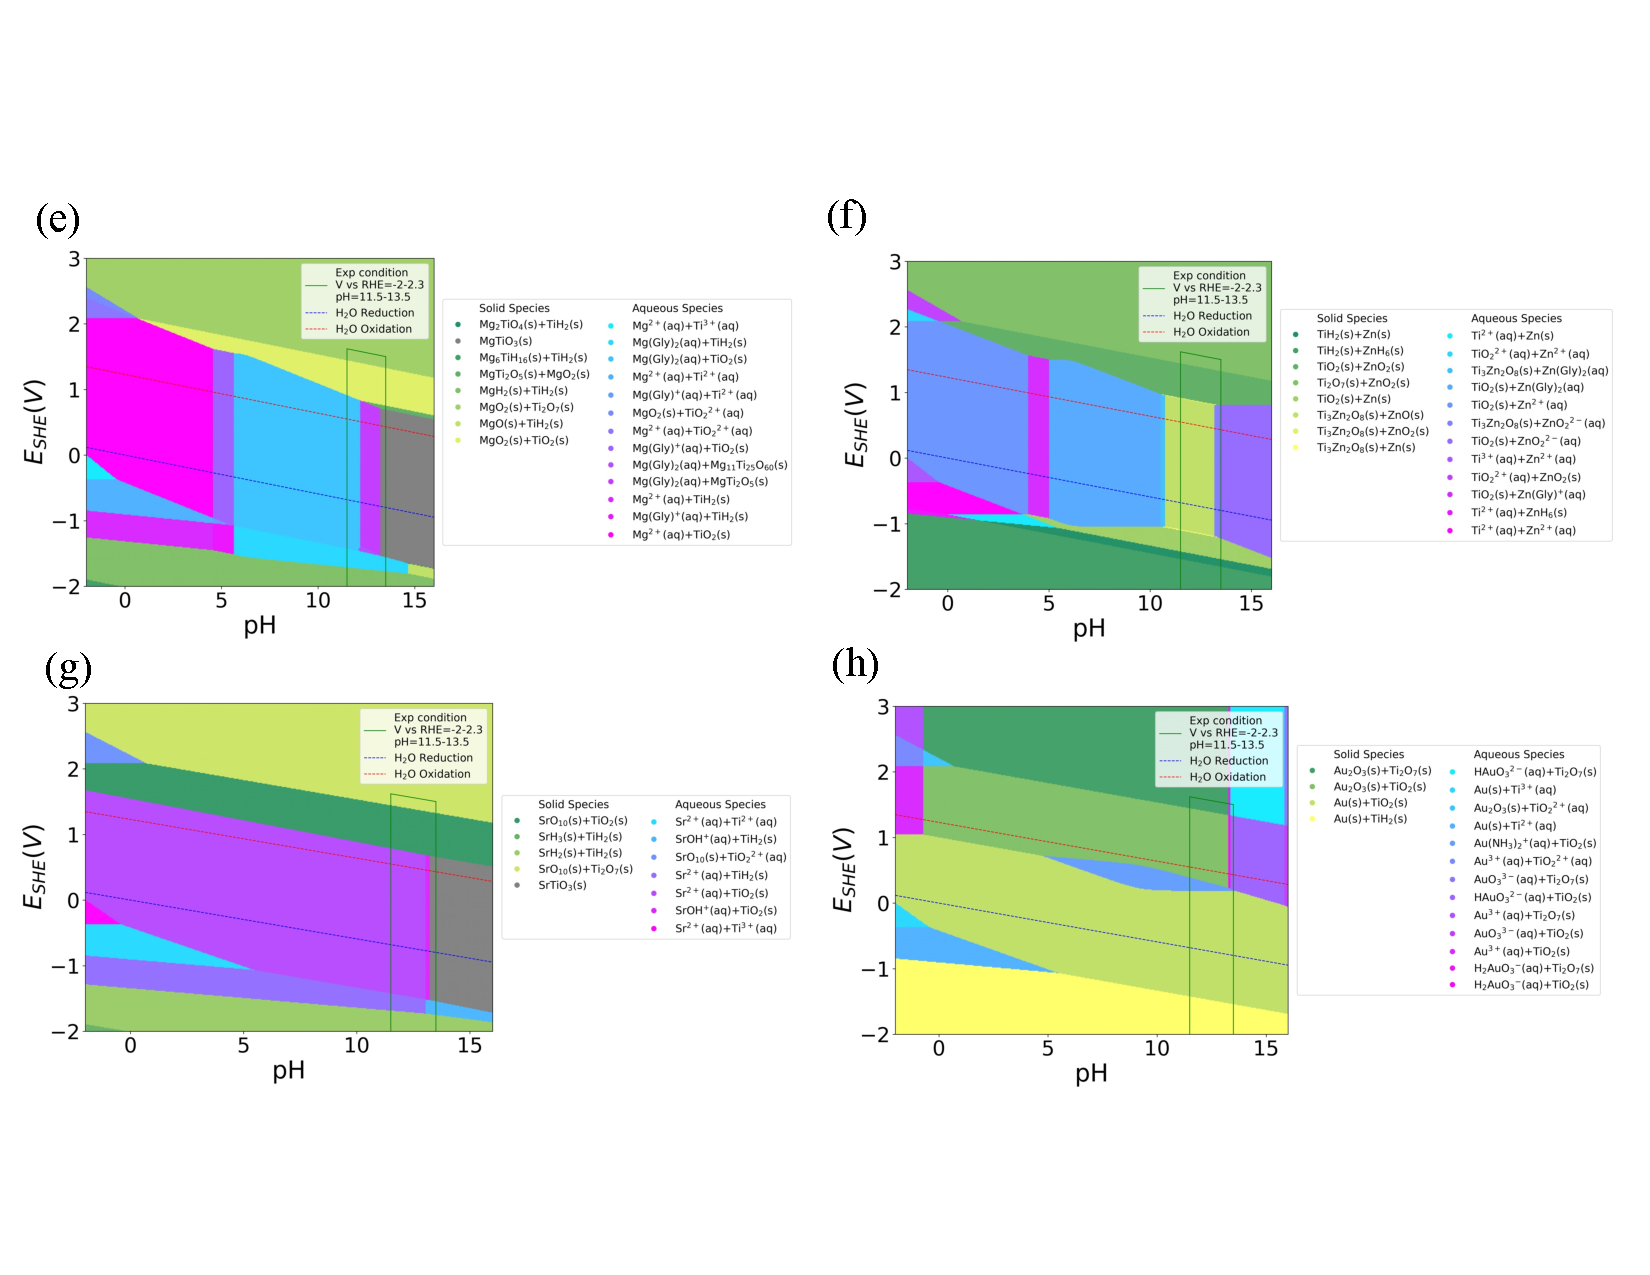
\includegraphics[width=1.1\textwidth]{Figures/alloy_pourbaix_diagrams/alloy_pourbaix_collage_2.pdf}}
\caption{Metal alloy Pourbaix diagrams: (e) Mg-Ti, (f) Zn-Ti, (g) Sr-Ti, (h) Au-Ti, with $\text{ion activity}=\num{1e-4}$M, $[\ce{NH3}]_{initial}= 0.02$M, $[\text{Gly}]_{initial}=0.005$M. The green box indicates the experimental condition at an applied potential of -2 to 2V vs RHE, pH = 11.5 to 13.5.}
\label{fig:alloy_pourbaix_collage_2}
\end{figure}
%%%%%%%%%%%%%%%%%%%%%%%%%%%%%%%%%%%%%%%%%%%%%%%%%%%%%%%%%%%%%%%%%

\subsubsection{Ni-Ti Alloy Stability}
Using an equiatomic composition constraint between titanium and nickel, the Pourbaix diagram reveals that a single stable oxide phase, \ce{TiNiO3}, dominates under EWAS-relevant pH and potential conditions in the presence of \ce{NH3} and glycine ligands. Compared to the Ni-only Pourbaix diagram (\ref{fig:Ni_Pourbaix_NH3_Gly}), the stability region of the \ce{Ni(Gly)_3^{-}} complex is reduced, with \ce{TiNiO3} occupying a broader region in the experimental pH range. This oxide phase also exhibits greater stability than the solvated \ce{Ni(OH)_3^-} species, remaining thermodynamically favored up to pH 14, thereby extending the passivation window compared to pure nickel. 

At lower pH values, the Ni–glycine complexes become more stable than the mixed-metal oxide, indicating that the stability of the oxide is pH-dependent and can be suppressed under more acidic conditions. Furthermore, at very low cyanide concentrations of \SI{1e-4}M (\Cref{fig:TiNi_alloy_Pourbaix}(b), the alloy oxide phase may dissolve into the highly stable \ce{Ni(CN)_4^{2-}}. Therefore, the presence of cyanide ligands could still promote Ni leaching, despite the formation of a passivating mixed-metal oxide layer.

Consistent with the report by Ding et al. \cite{Ding2018ElectrochemicalStates}, the thermodynamically stable oxide formed in aqueous solutions is primarily composed of \ce{TiNiO3}. However, experimental studies \cite{Huang2005SurfaceAcidity, Clarke2006InfluenceRelease, Carroll2003CorrosionEnvironments} have identified \ce{TiO2} and NiO as the main components of the oxide layer. According to Ding et al., \ce{TiO2} and NiO can further react to form the more stable ternary oxide \ce{TiNiO3}. Additional experimental investigations and surface phase diagram analyses are needed to validate the applicability of \ce{TiNiO3} as a candidate for EWAS electrodes and to understand its role in corrosion resistance mechanisms better.

%%%%%%%%%%%%%%%%%%%%%%%%%%%%%%%%% TiNi Alloy %%%%%%%%%%%%%%%%%%%%%%%%%%%%%%%%%
\begin{figure}[htbp]
    \centering
    \begin{subfigure}[b]{0.45\textwidth}
        \label{fig:TiNi_Pourbaix_NH3_Gly}
        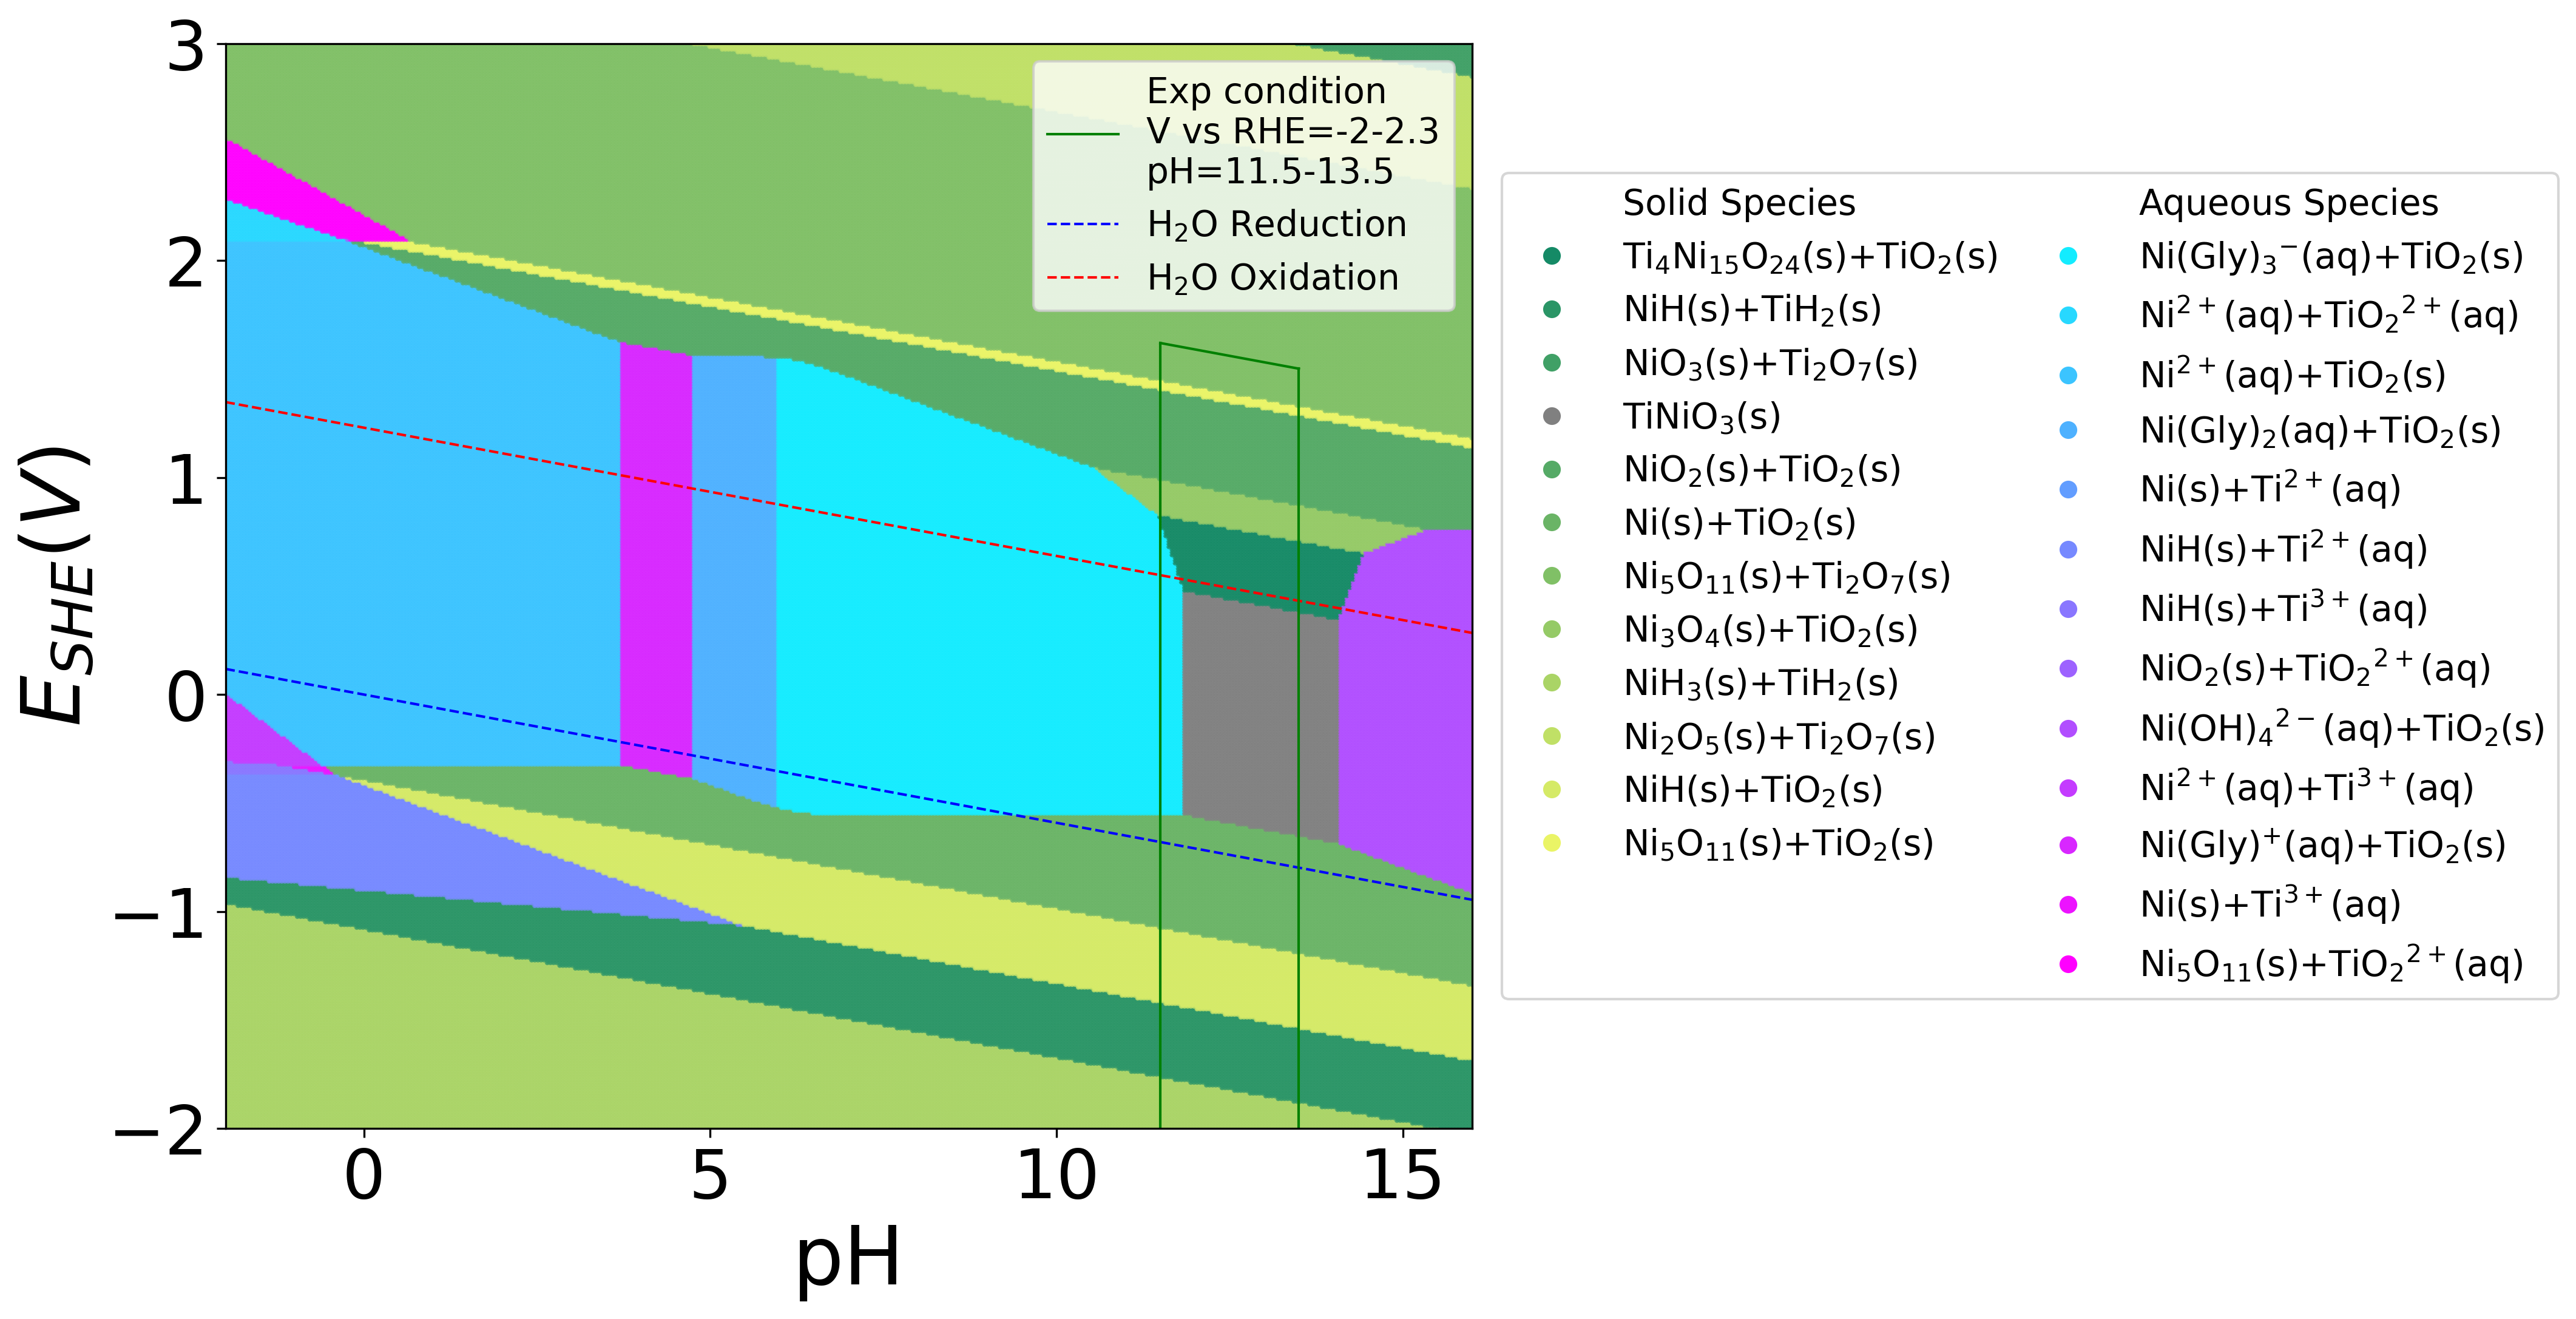
\includegraphics[width=\textwidth]
        {Figures/alloy_pourbaix_diagrams/Ti_Ni_alloy_Ti0.5 Ni0.5_NH3=0.02M_Gly=0.005M_CN=0M_activity=1e-04M.png}
       % \par\medskip
    \end{subfigure}
    \begin{subfigure}[b]{0.45\textwidth}
        \label{fig:TiNi_Pourbaix_NH3_Gly_CN}
        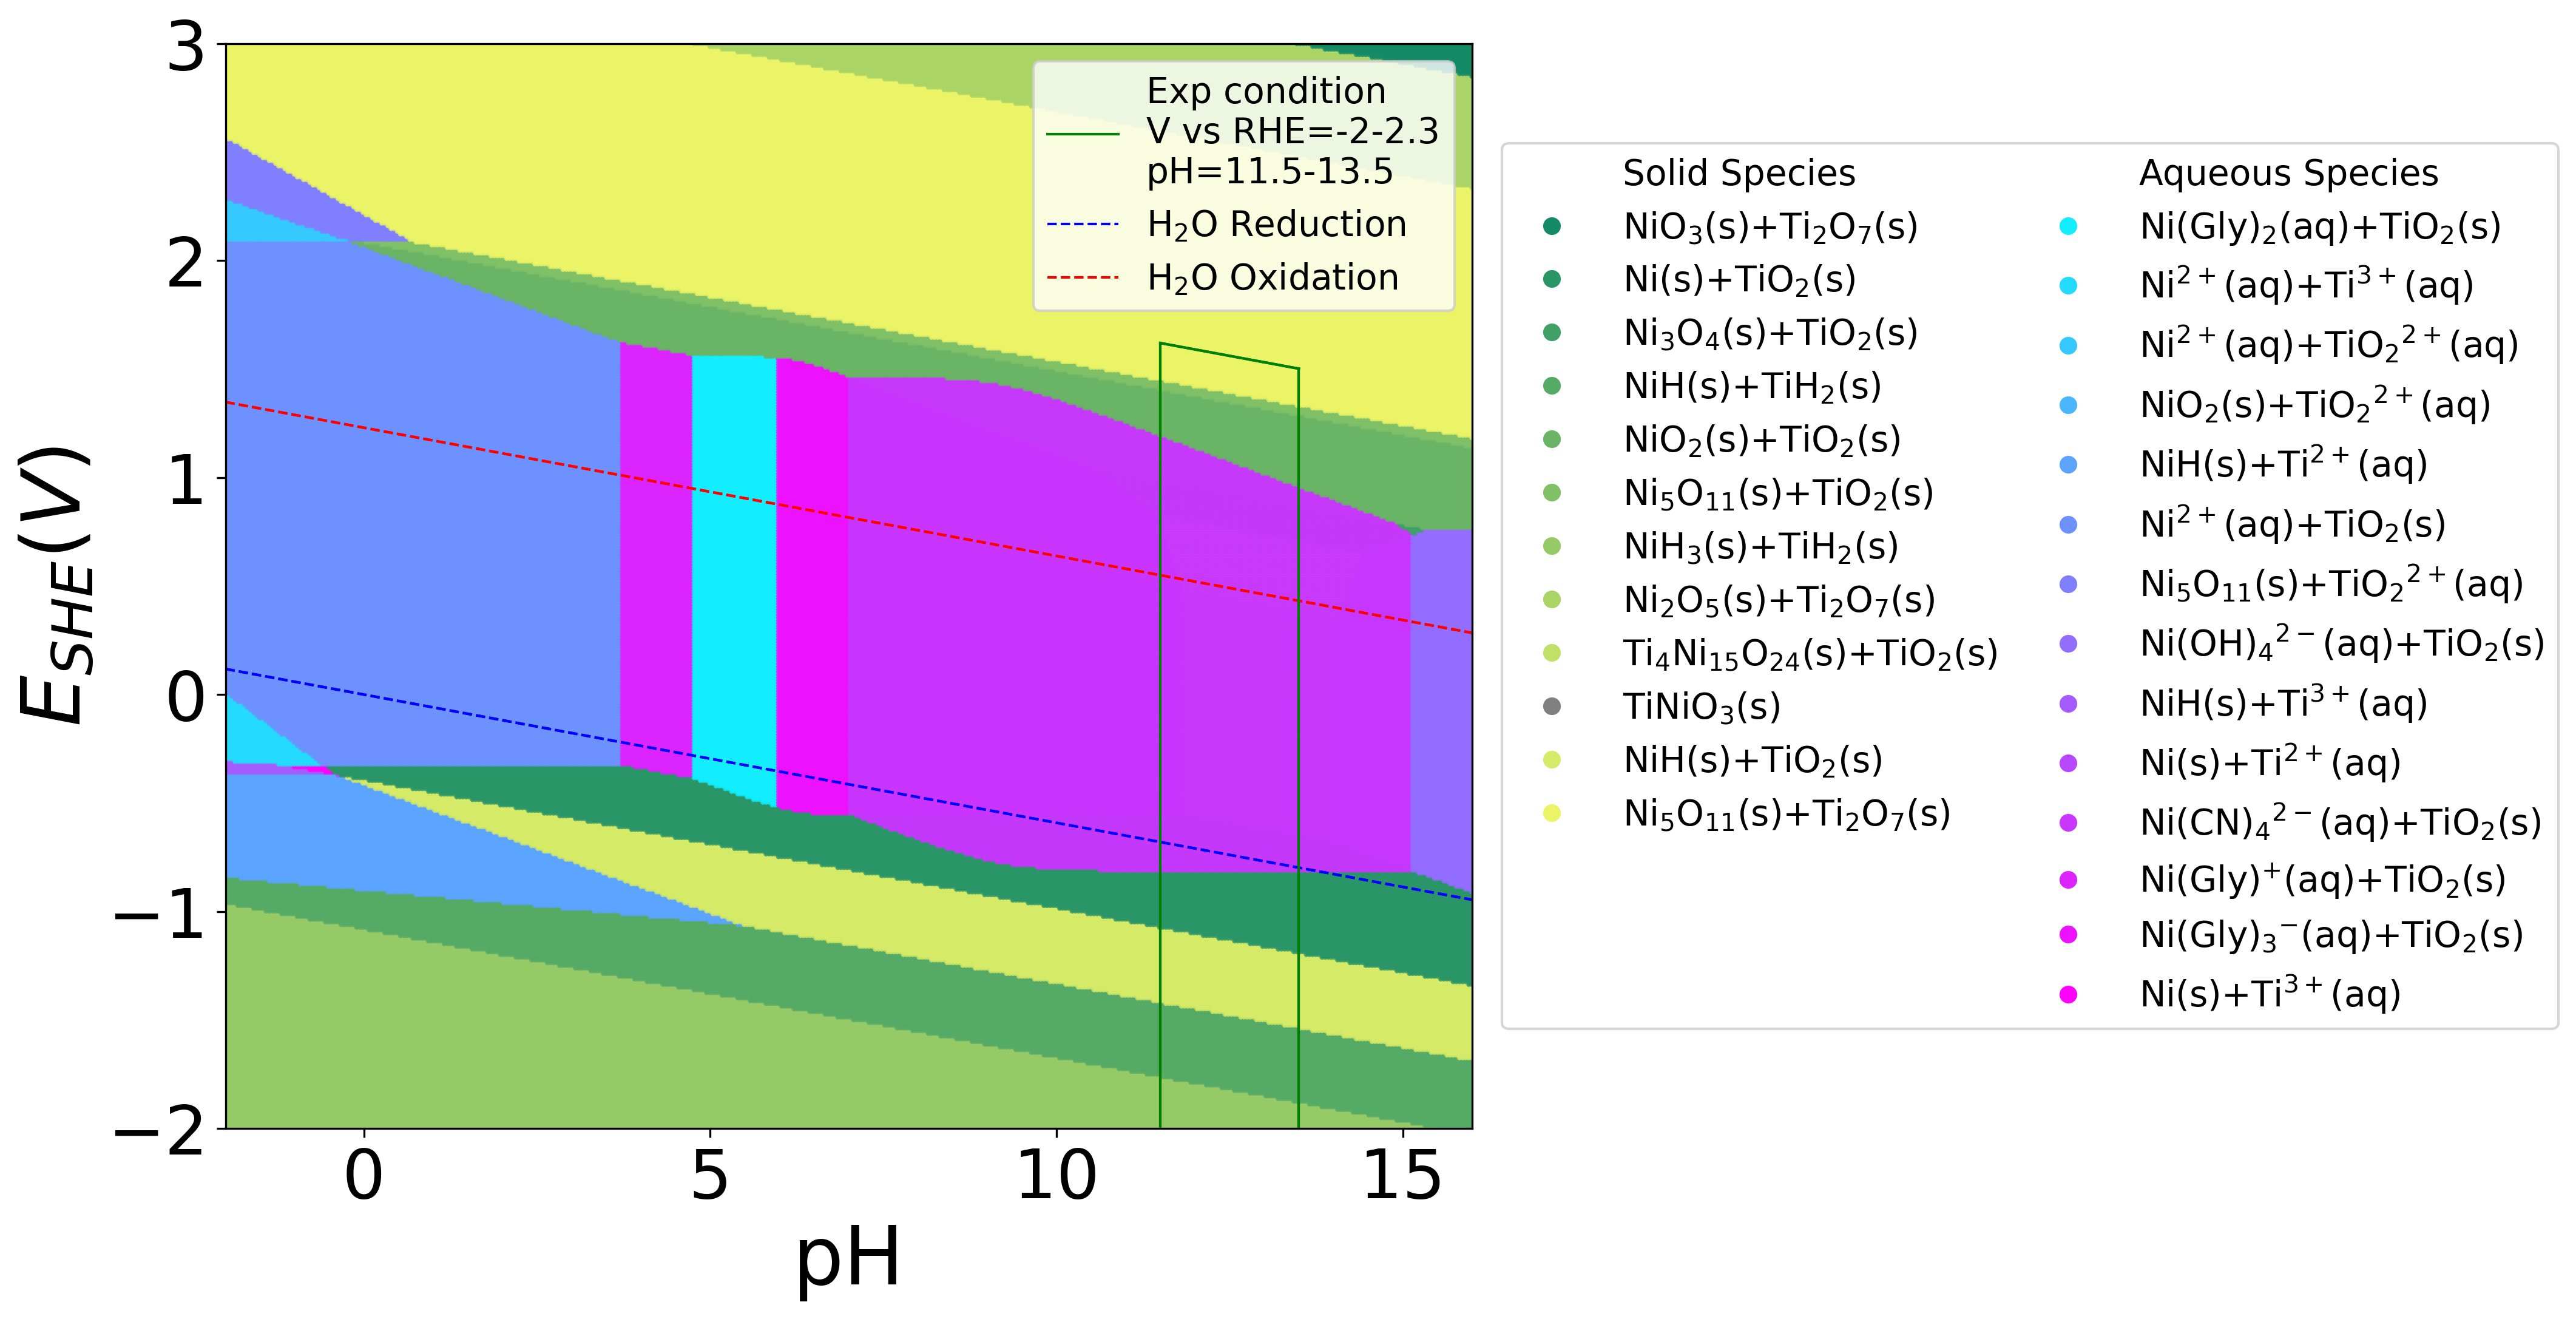
\includegraphics[width=\textwidth]{Figures/alloy_pourbaix_diagrams/Ti_Ni_alloy_Ti0.5 Ni0.5_NH3=0.02M_Gly=0.005M_CN=0.0001M_activity=1e-04M.png}
       % \par\medskip   
    \end{subfigure}
    \caption{Ni-Ti alloy Pourbaix diagrams with $\text{ion activity} = \num{1e-4}$: (a) $[\ce{NH3}]_\text{initial} = 0.02$~M, $[\text{Gly}]_\text{initial} = 0.005$~M; (b) $[\ce{NH3}]_\text{initial} = 0.02$~M, $[\text{Gly}]_\text{initial} = 0.005$~M, and $[\ce{CN^-}]_\text{initial} = \num{1e-4}$~M. A fixed reference stoichiometry of Ti:Ni = 1:1 was applied as a compositional constraint when generating the alloy Pourbaix diagrams. The green box highlights the experimentally relevant region, defined by an applied potential of \SIrange{-2}{2}{V} vs. RHE and a pH range of 11.5 to 13.5. Thermodynamically stable alloy regions are shaded in grey.}
    \label{fig:TiNi_alloy_Pourbaix}
\end{figure}


\subsubsection{Ti-Cu Alloys}
The Cu–Ti Pourbaix diagrams with nitrogen-containing ligands are shown in \Cref{fig:TiCu_alloy_Pourbaix}. As noted earlier, Cu and Ti's alloy phases do not show up in these diagrams, so their Pourbaix diagrams primarily reflect the overlap between the individual stability regions of copper and titanium oxides.

In the presence of \ce{NH3} and glycine, coexisting copper oxide and titanium oxide phases demonstrate good thermodynamic stability across the EWAS-relevant pH and potential window. This is consistent with the pure Cu Pourbaix diagram in \Cref{fig:Cu_Pourbaix_NH3_Gly}, where copper oxides are stable from pH 9 to 14.5 under both reductive and oxidative conditions. When cyanide is introduced, the \ce{[Cu(CN)_3]^{2-}} complex can form and coexist with \ce{TiO2}, spanning a broad pH range from 9 to 15.5.

Alloying Ti with Cu has been studied primarily to improve titanium’s mechanical properties \cite{Osorio2010ElectrochemicalApplications, Wang2019OptimizationImplant, Fotopoulos2024ModelingAlloys}. However, its electrochemical applications and corrosion mechanisms under EWAS-relevant conditions remain relatively underexplored \cite{Nagarjuna1997EffectCopper, Suzuki2003ElectricalAlloys, Vorotilo2020DFTRe-oxidation, Li2025ApplicationReview}, with most research focused on extreme environments such as deep-sea or biomedical settings. Brunelli et al. \cite{Brunelli2001ElectrochemicalAlloys} reported that a porous copper-rich layer in the alloy enhances electrocatalytic activity toward the hydrogen evolution reaction, particularly in alkaline media, owing to copper’s inherent stability under such conditions. The observed thermodynamic stability of Cu and Ti oxides in Pourbaix analysis suggests that these alloys are potentially interesting candidates to improve the corrosion resistance and long-term stability of catalysts under EWAS operating conditions.

%%%%%%%%%%%%%%%%%%%%%%%%%%%%%%%%% TiCu Alloy %%%%%%%%%%%%%%%%%%%%%%%%%%%%%%%%%
\begin{figure}[htbp]
    \centering
    \begin{subfigure}[b]{0.45\textwidth}
        \subcaption{}\label{fig:TiCu_Pourbaix_NH3_Gly}
        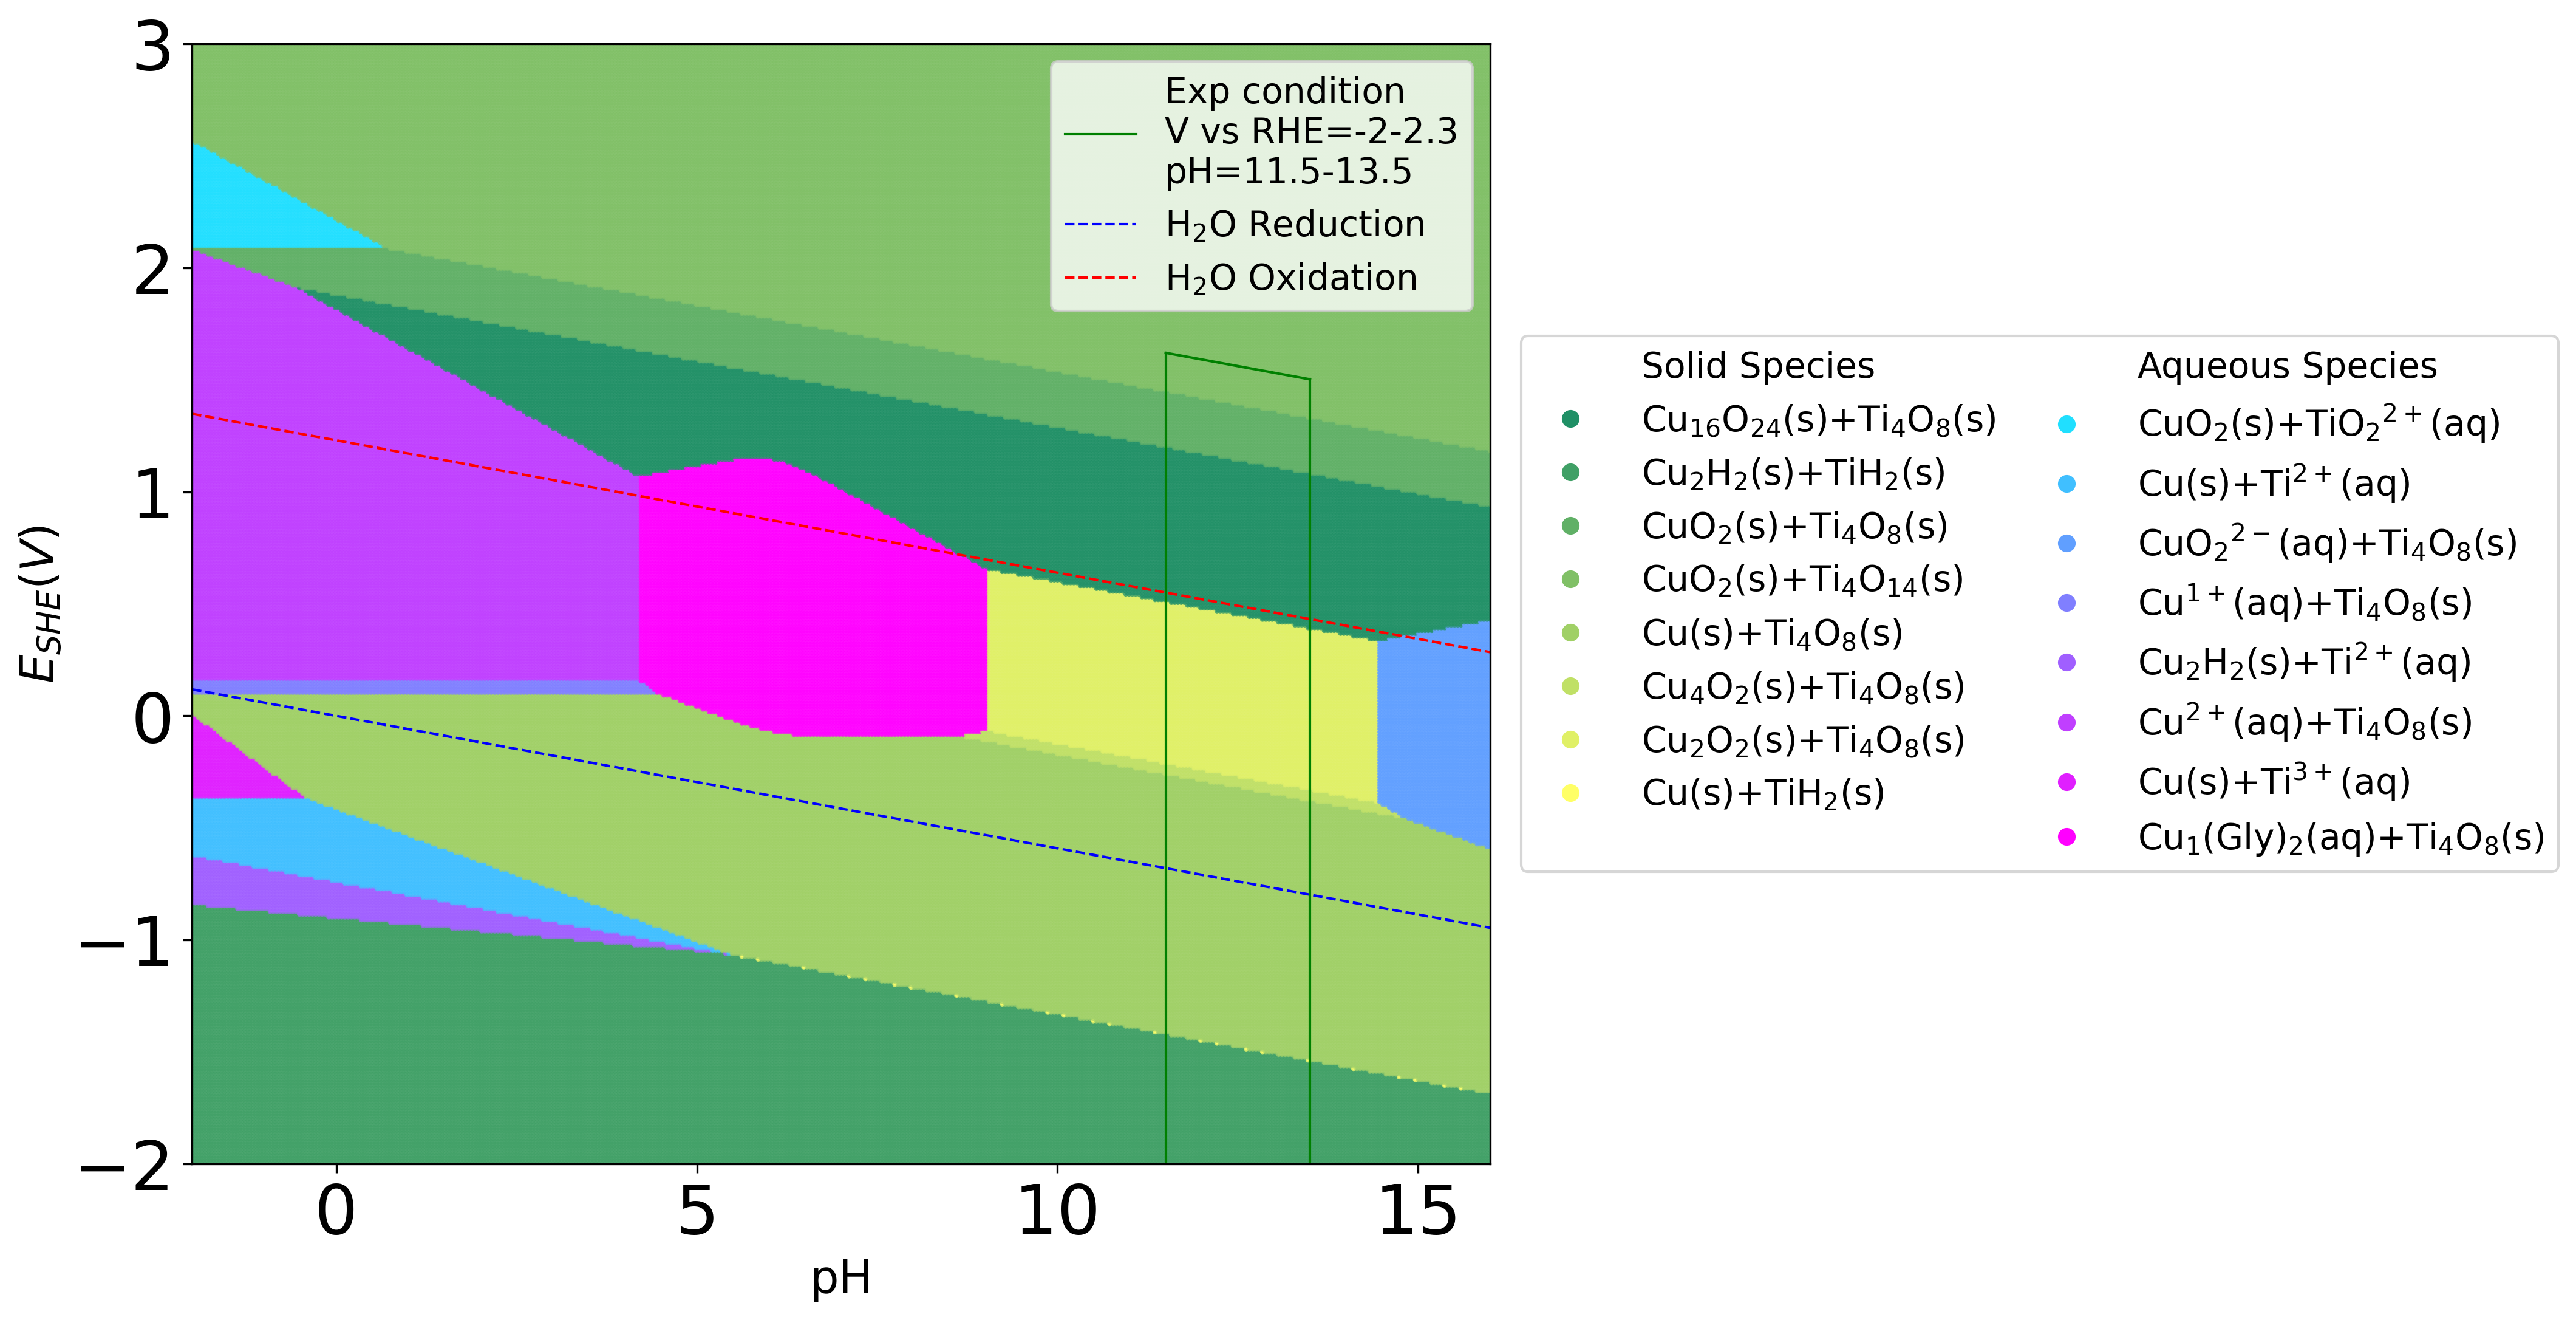
\includegraphics[width=\textwidth]
        {Figures/alloy_pourbaix_diagrams/Ti_Cu_alloy_Ti0.5 Cu0.5_NH3=0.02M_Gly=0.005M_CN=0M_activity=1e-04M.png}
       % \par\medskip
    \end{subfigure}
    \begin{subfigure}[b]{0.45\textwidth}
        \subcaption{}\label{fig:TiCu_Pourbaix_NH3_Gly_CN}
        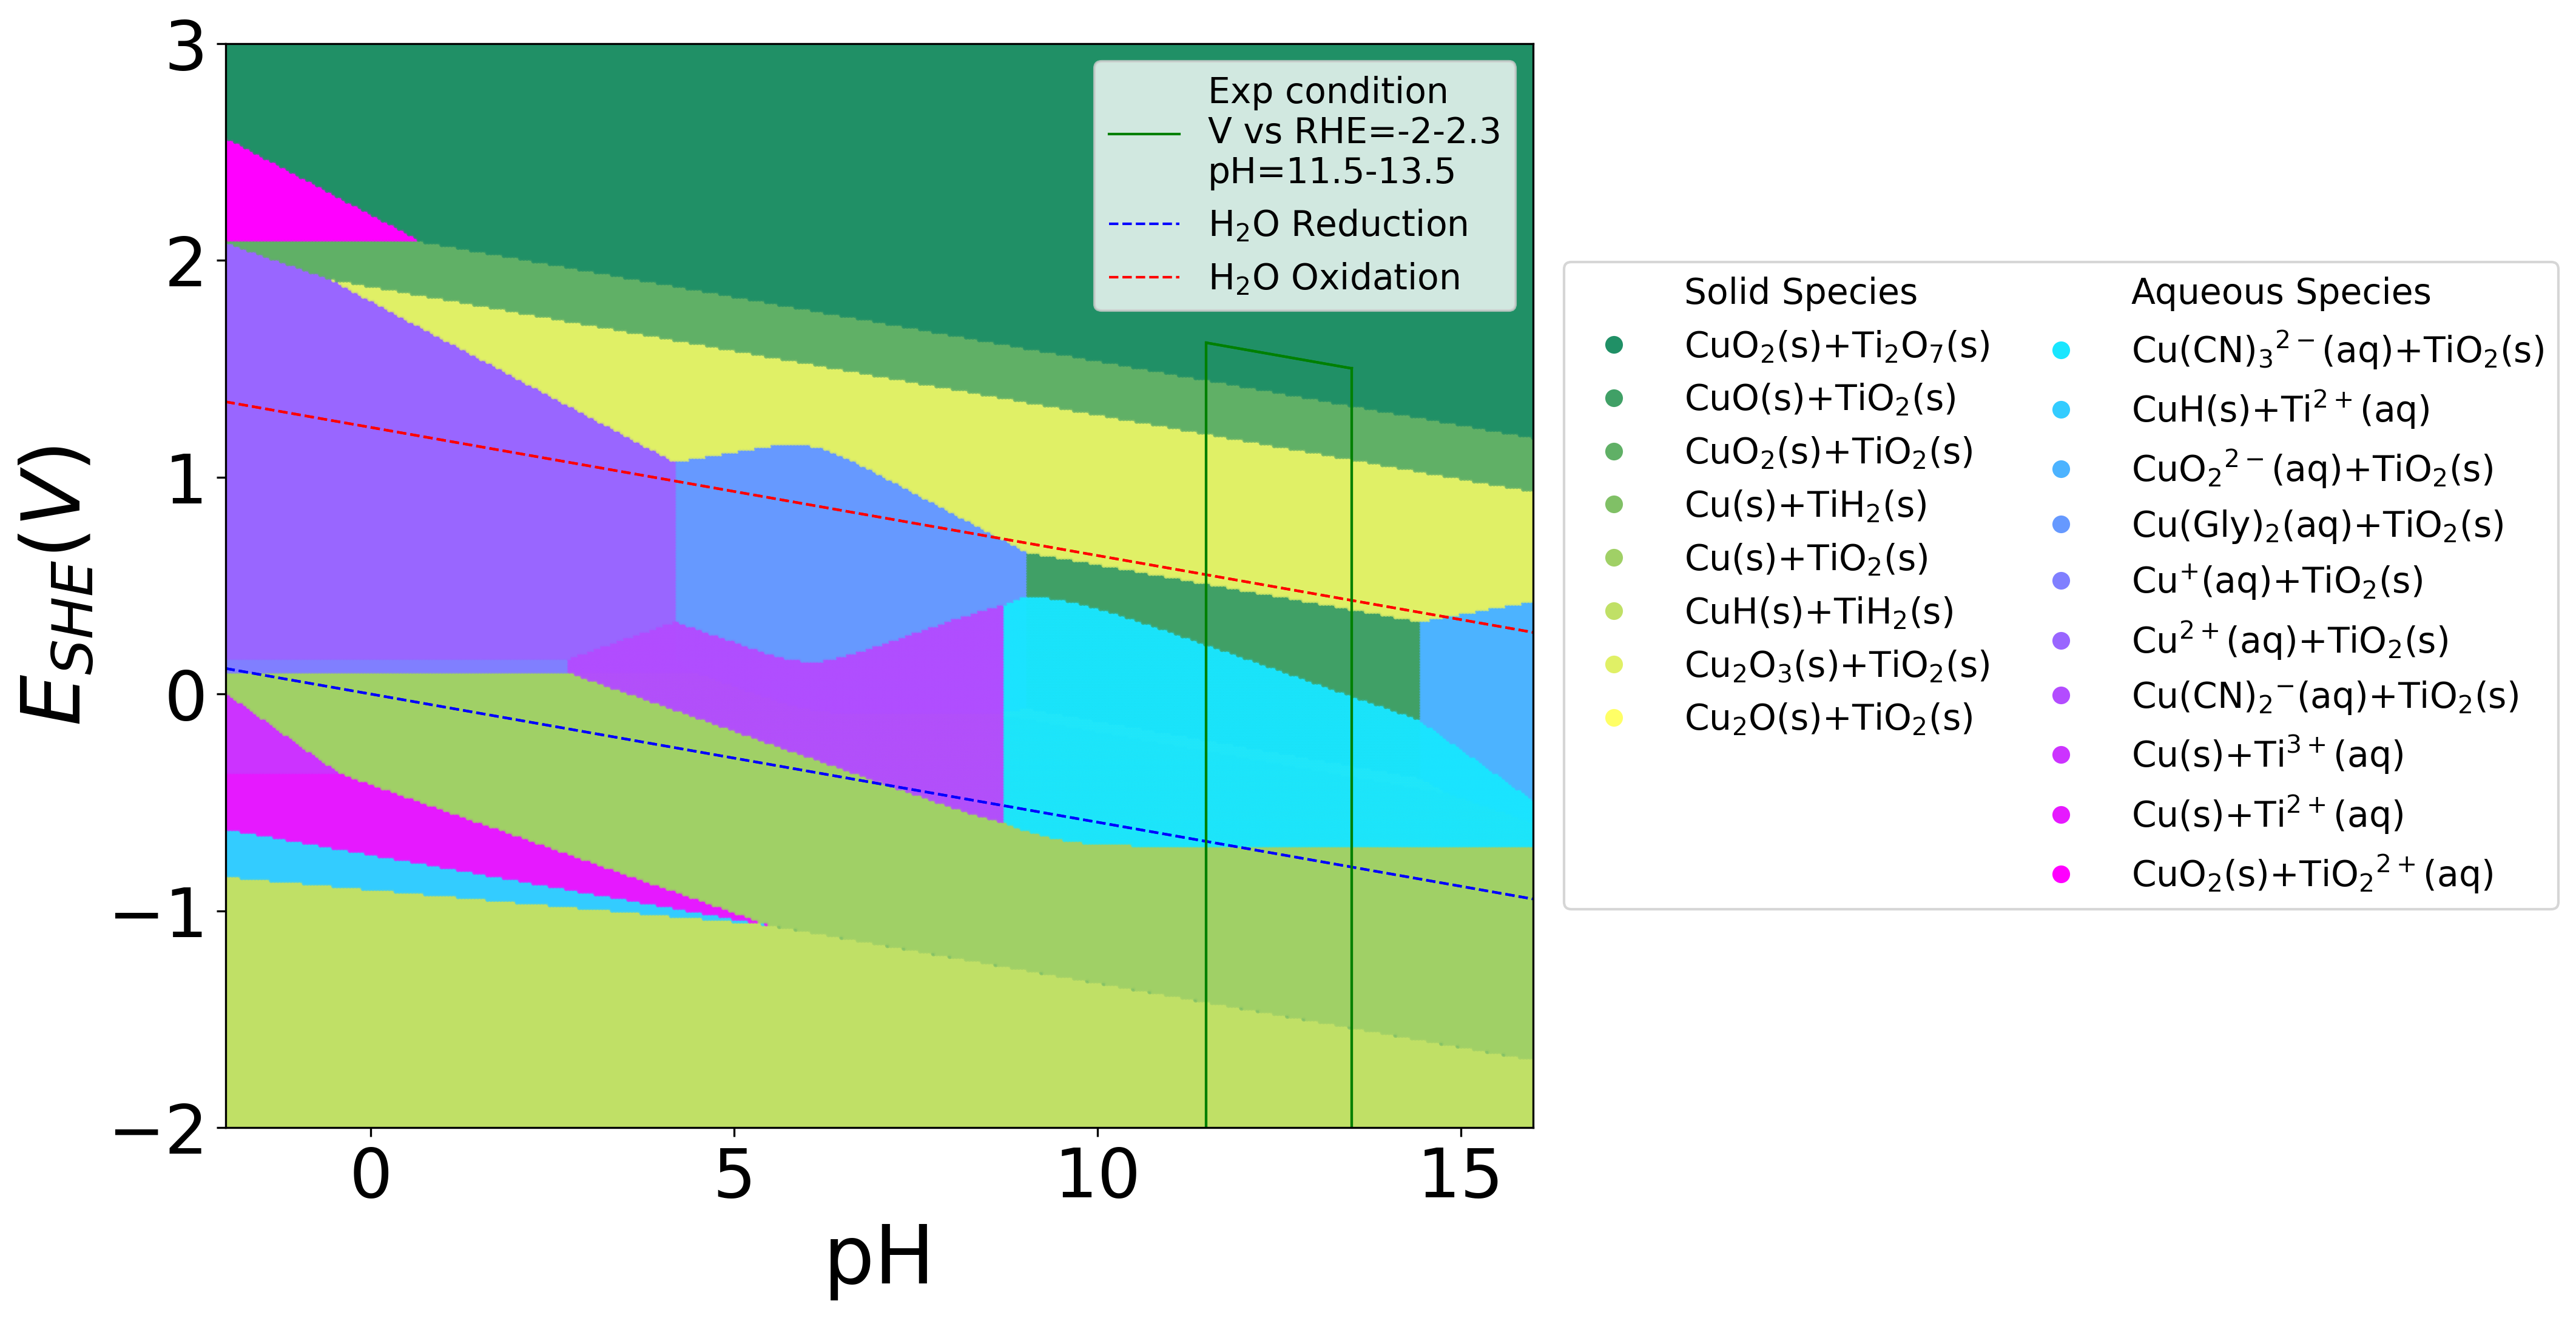
\includegraphics[width=\textwidth]{Figures/alloy_pourbaix_diagrams/Ti_Cu_alloy_Ti0.5 Cu0.5_NH3=0.02M_Gly=0.005M_CN=0.0001M_activity=1e-04M.png}
       % \par\medskip   
    \end{subfigure}
    \caption{Cu-Ti alloy Pourbaix diagrams with $\text{ion activity} = \num{1e-4}$: (a) $[\ce{NH3}]_\text{initial} = 0.02$~M, $[\text{Gly}]_\text{initial} = 0.005$~M; (b) $[\ce{NH3}]_\text{initial} = 0.02$~M, $[\text{Gly}]_\text{initial} = 0.005$~M, and $[\ce{CN^-}]_\text{initial} = \num{1e-4}$~M. A fixed reference stoichiometry of Ti:Cu = 1:1 was applied as a compositional constraint when generating the alloy Pourbaix diagrams. The green box highlights the experimentally relevant region, defined by an applied potential of \SIrange{-2}{2}{V} vs. RHE and a pH range of 11.5 to 13.5. Thermodynamically stable alloy regions are shaded in grey.}
    \label{fig:TiCu_alloy_Pourbaix}
\end{figure}


\subsubsection{Pd alloys}
Pd alloys Pourbaix diagrams are shown in \Cref{fig:alloy_pourbaix_collage_3,fig:alloy_pourbaix_collage_4}. Alloys of Pd with Ag, Pt, Au, and Cu exhibit favorable thermodynamic stability across the targeted potential and pH ranges. Among these, Ag shows a large stability region for its solvated ion phase (\ce{Ag^+}) and glycine complexes at pH below 12, although the overlap with the EWAS-relevant window is limited. Pt, which is intrinsically resistant to leaching by \ce{NH3} and glycine ligands, forms stable alloy phases with Pd that maintain strong thermodynamic stability. These properties make Pd–Pt alloys particularly interesting candidates for further experimental evaluation under EWAS conditions.

The Pd–Au alloy \ce{Pd3Au} is stable within the experimental potential range from –1 to 0.3 V vs. RHE. However, this region does not overlap with the stability window of the \ce{[Au(NH3)_2]^+} complex, suggesting that alloying with Pd may not suppress Au leaching via ammonia complexation. Nevertheless, due to Au’s known catalytic activity toward glycine and other nitrogen-containing species, Pd–Au alloys remain promising candidates for experimental investigation.

The Cu–Pd alloy system also displays significant stability across EWAS-relevant conditions. Notably, \ce{CuPdO2} shows a broad stability region, as seen in \Cref{fig:alloy_pourbaix_collage_3}(d), and can even suppress the stability of glycine–Pd complexes. Given that Cu resists leaching by \ce{NH3} and glycine under these conditions, Cu–Pd alloys offer a promising combination of durability and catalytic potential.

Other Pd alloys, such as Zn–Pd and Sr–Pd, can form stable phases, but their solvated ion species (\ce{Zn^2+}, \ce{Sr^2+}) are thermodynamically favored under less alkaline and both reductive and oxidative potentials, reducing their resistance to dissolution. Mg does not form stable alloy phases with Pd, so the corresponding diagrams largely reflect the overlay of the individual metal Pourbaix diagrams.

Fe forms a stable \ce{FePd3} alloy that can coexist with bulk Fe and Pd oxides. Its stability is more pronounced under reductive conditions, consistent with previous reports that Fe–Pd alloys exhibit enhanced activity toward the oxygen reduction reaction (ORR) \cite{Ou2015DesignStudy}.

%%%%%%%%%%%%%%%%%%%%%%%%%%%%%%%%% Collage of Pd Alloy Pourbaix Diagrams %%%%%%%%%%%%%%%%%%%%%%%%%%%%%%%%%
\begin{figure}[htbp]
\centering
\makebox[\textwidth][c]{%g
        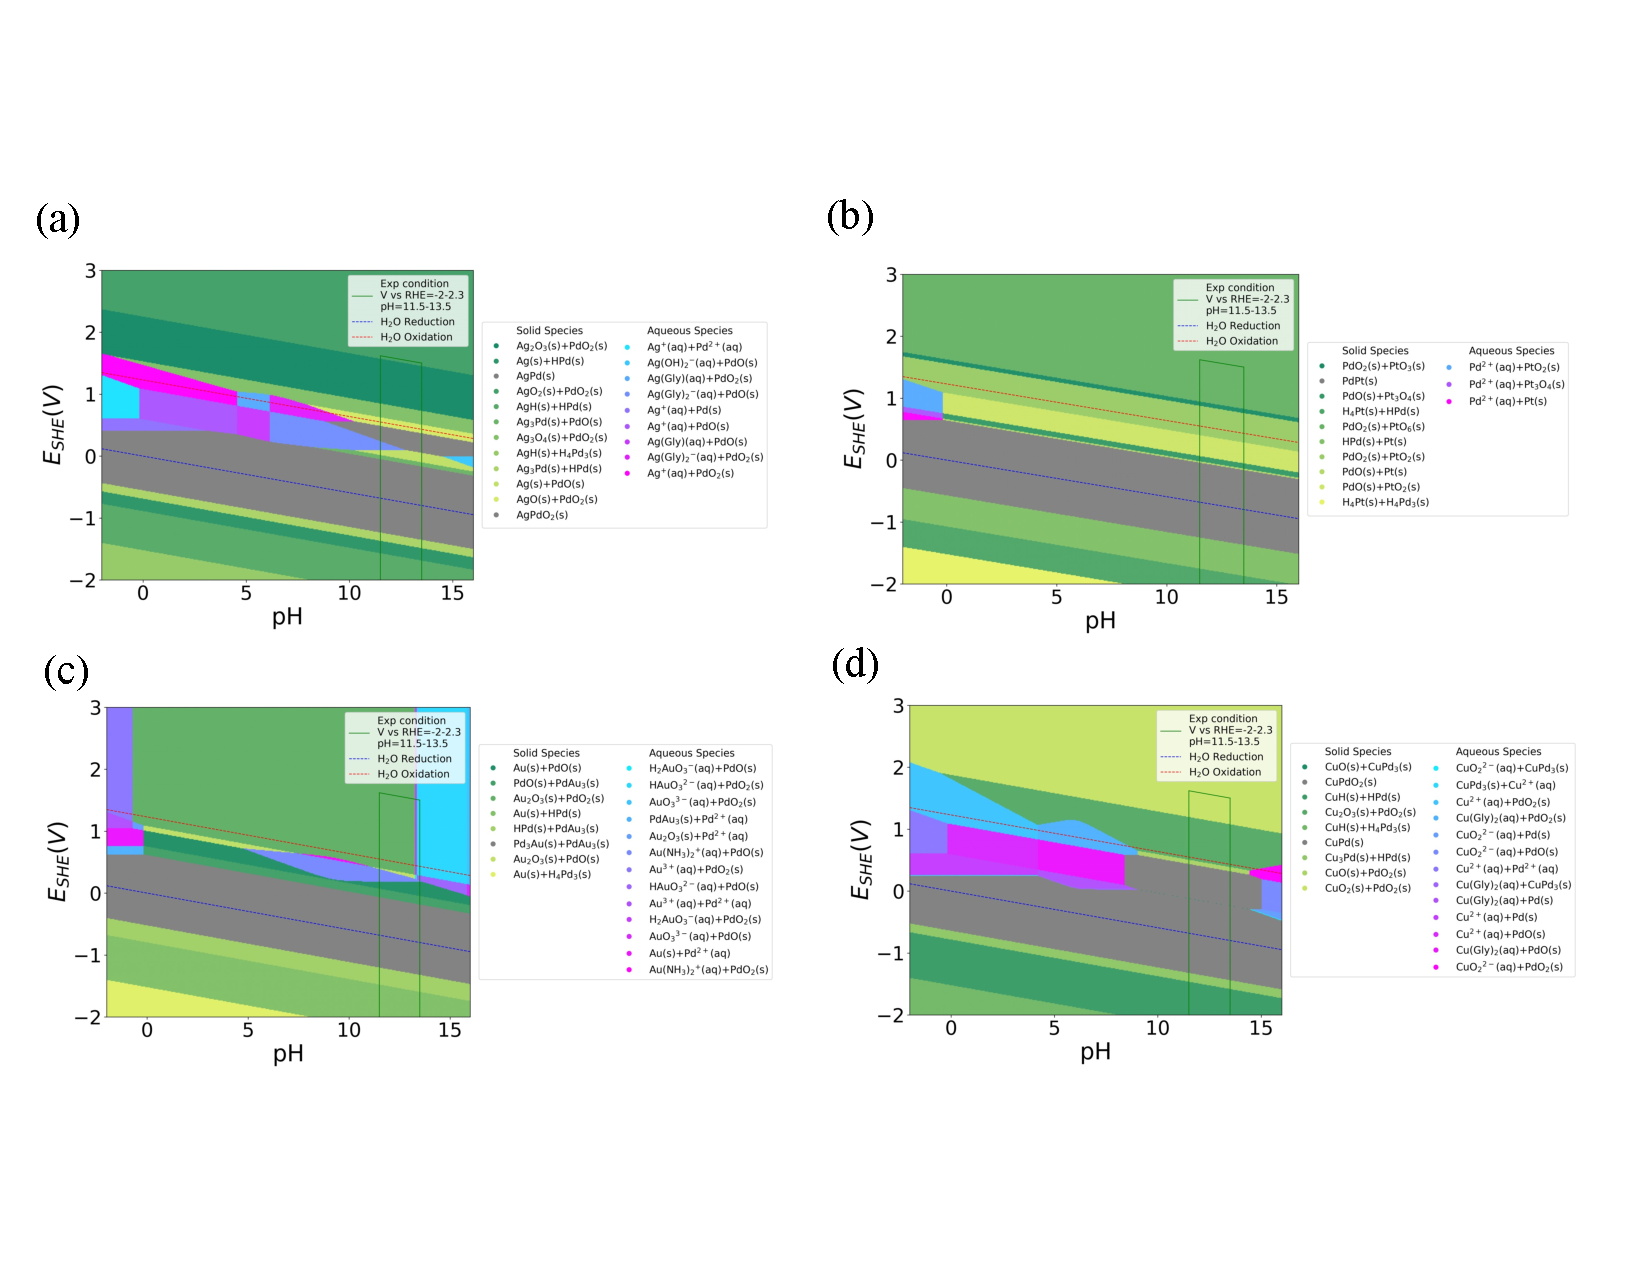
\includegraphics[width=1.1\textwidth]{Figures/alloy_pourbaix_diagrams/alloy_pourbaix_collage_3.pdf}}
\caption{Metal alloy Pourbaix diagrams: (a) Ag-Pd, (b) Pt-Pd, (c) Au-Pd, (d) Cu-Pd, with $\text{ion activity}=\num{1e-4}$M, $[\ce{NH3}]_{initial}= 0.02$M, $[\text{Gly}]_{initial}=0.005$M. The green box indicates the experimental condition at an applied potential of -2 to 2V vs RHE, pH = 11.5 to 13.5.}
\label{fig:alloy_pourbaix_collage_3}
\end{figure}

\begin{figure}[htbp]
\centering
\makebox[\textwidth][c]{%g
        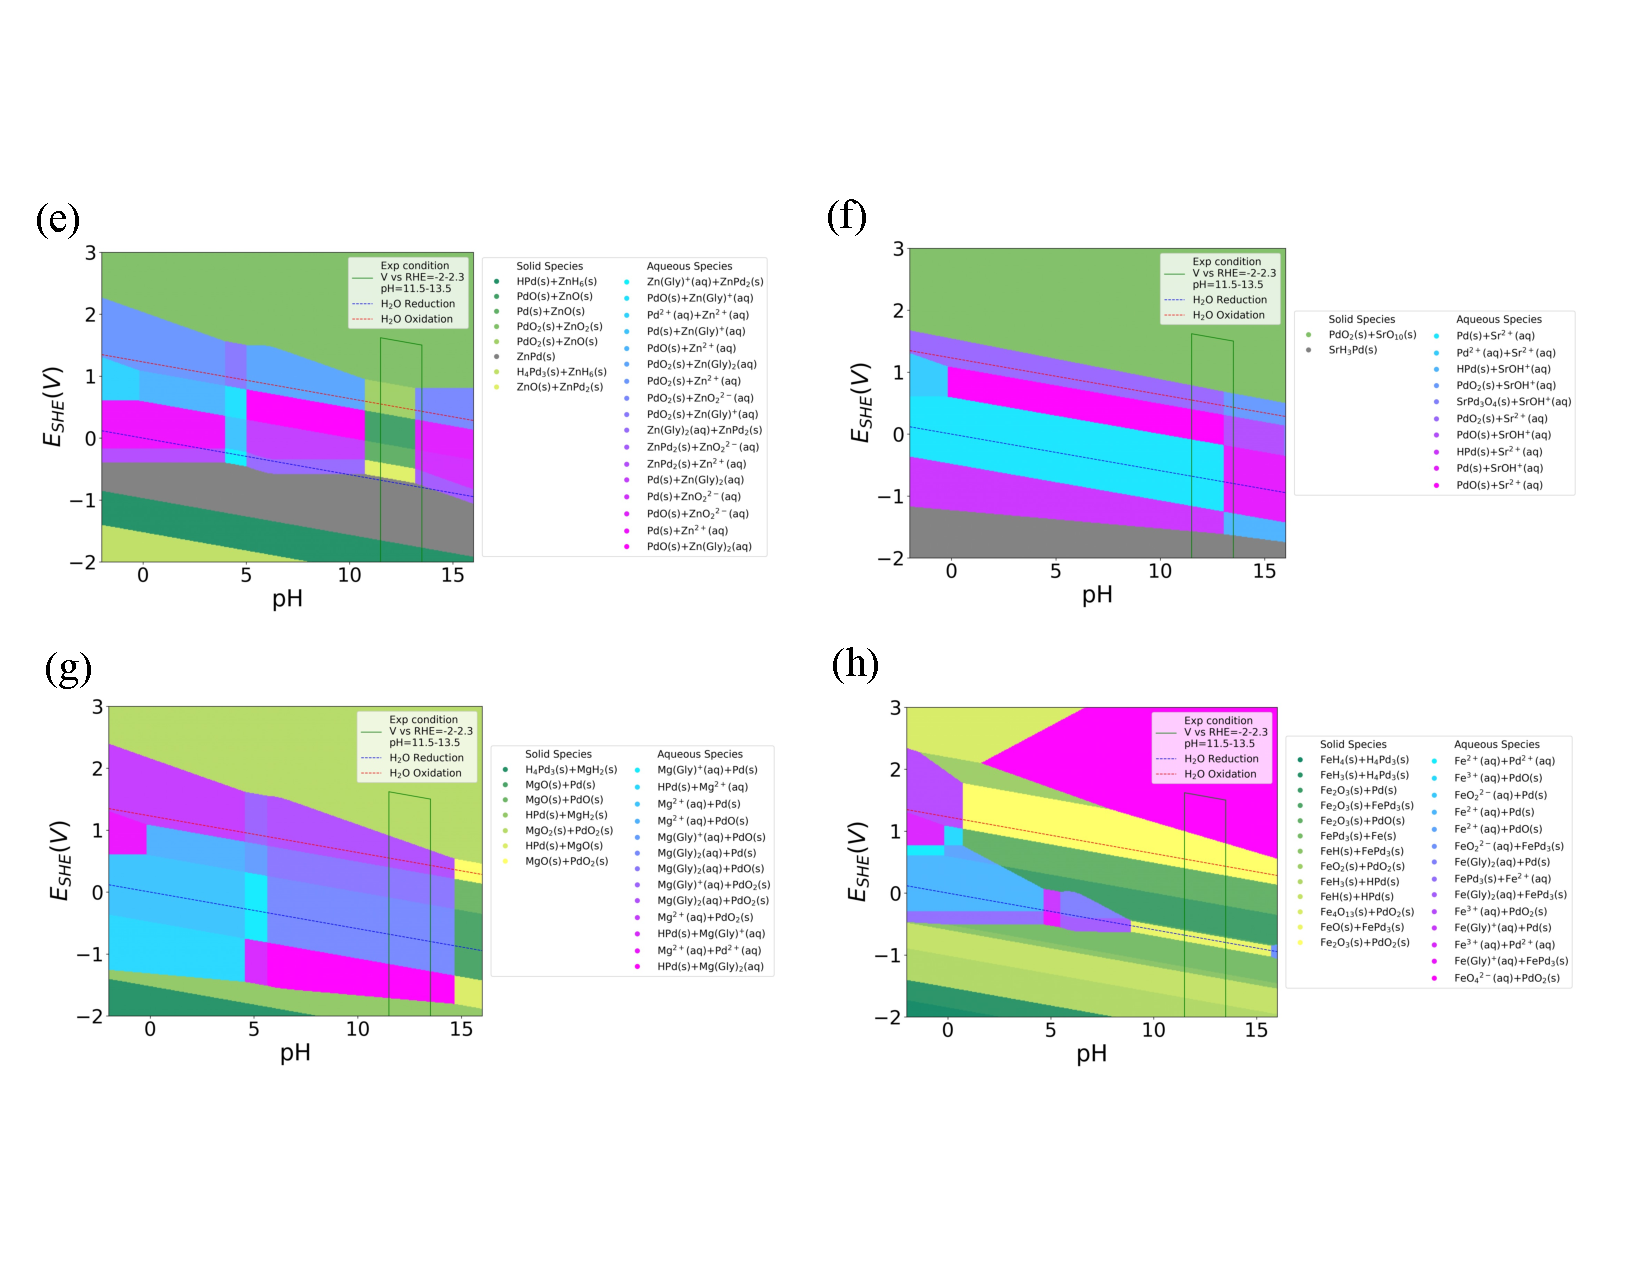
\includegraphics[width=1.1\textwidth]{Figures/alloy_pourbaix_diagrams/alloy_pourbaix_collage_4.pdf}}
\caption{Metal alloy Pourbaix diagrams: (e) Zn-Pd, (f) Sr-Pd, (g) Mg-Pd, (h) Fe-Pd, with $\text{ion activity}=\num{1e-4}$M, $[\ce{NH3}]_{initial}= 0.02$M, $[\text{Gly}]_{initial}=0.005$M. The green box indicates the experimental condition at an applied potential of -2 to 2V vs RHE, pH = 11.5 to 13.5.}
\label{fig:alloy_pourbaix_collage_4}
\end{figure}
%%%%%%%%%%%%%%%%%%%%%%%%%%%%%%%%%%%%%%%%%%%%%%%%%%%%%%%%%%%%%%%%%
\subsubsection{Au-Pd Alloy Stability}

As shown in \Cref{fig:PdAu_Pourbaix_NH3_Gly}, two Pd–Au alloys, \ce{PdAu3} and \ce{Pd3Au}, are predicted to be thermodynamically stable within the experimentally relevant pH and potential window. In this region, the \ce{[Au(NH3)_2]^+} complex is also stable and can coexist with PdO between 0.5 and 0.8~V vs. RHE. However, the formation of stable Au–Pd alloys does not significantly shift the stability domains of the Au–ammonia or Au–glycine complexes, as these ligand-bound species occupy regions outside the alloy stability window. Similarly, the passivation regions of both Au and Pd remain largely unchanged, since the alloy stability domains lie below the equilibrium dissolution potentials of the individual metals.

As shown in \Cref{fig:PdAu_Pourbaix_NH3_Gly}(b), both gold- and palladium–cyanide complexes, \ce{Au(CN)_2^-} and \ce{Pd(CN)_4^{2-}}, can coexist with Pd–Au alloys and \ce{PdO2} under EWAS-relevant conditions. These ligand-stabilized species reduce the stability window of \ce{PdAu3} and \ce{Pd3Au}, particularly under oxidative and alkaline environments.

In electrocatalysis, alloying Au with Pd has been shown to enhance Pd’s activity and durability, particularly for methanol oxidation, by modulating Pd’s structural and electronic properties \cite{Hoshi2006StructuralPalladium, Kelly2018UnderstandingReaction, Aota2023RevealingTomography}. While Pd offers good thermodynamic stability under EWAS conditions, it often exhibits limited catalytic activity for oxidation reactions. In contrast, Au demonstrates high activity toward nitrogen-containing compounds but suffers from leaching and corrosion in nitrogen-rich media. Therefore, Pd–Au alloys represent an intersting material class that may balance activity and durability.


%%%%%%%%%%%%%%%%%%%%%%%%%%%%%%%%% PdAu Alloy %%%%%%%%%%%%%%%%%%%%%%%%%%%%%%%%%
\begin{figure}[htbp]
    \centering
    \begin{subfigure}[b]{0.45\textwidth}
        \subcaption{}\label{fig:PdAu_Pourbaix_NH3_Gly}
        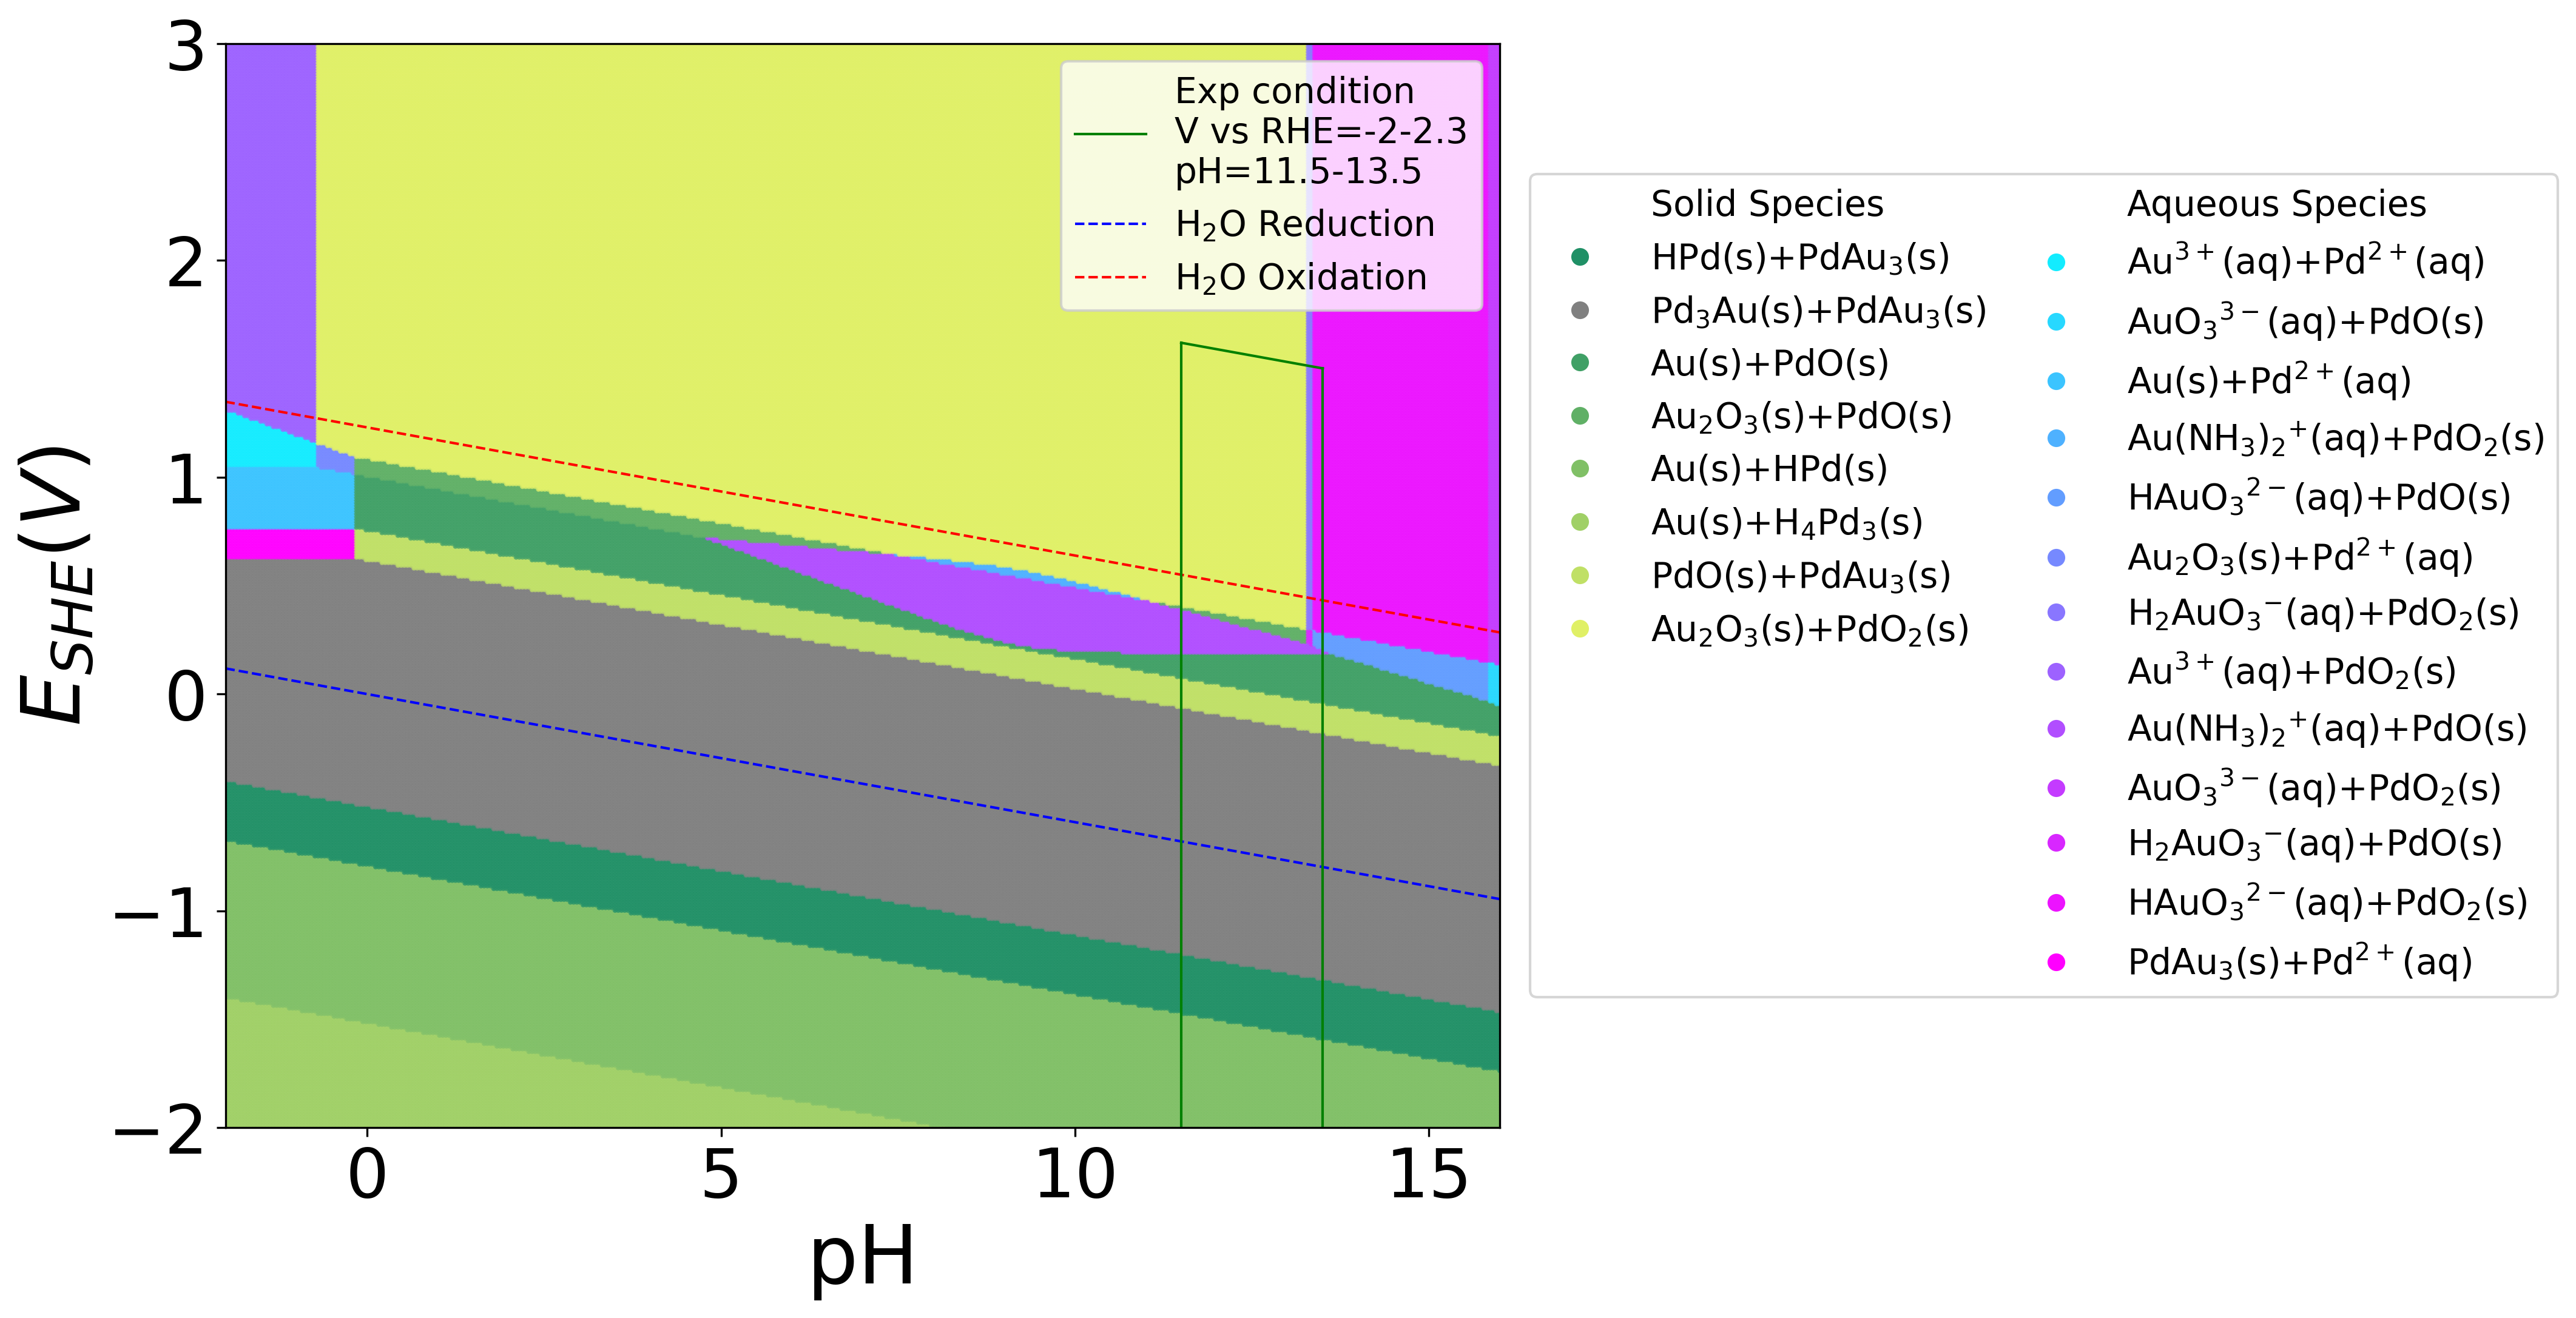
\includegraphics[width=\textwidth]
        {Figures/alloy_pourbaix_diagrams/Pd_Au_alloy_Pd0.5 Au0.5_NH3=0.02M_Gly=0.005M_CN=0M_activity=1e-04M.png}
       % \par\medskip
    \end{subfigure}
    \begin{subfigure}[b]{0.45\textwidth}
        \subcaption{}\label{fig:PdAu_Pourbaix_NH3_Gly_CN}
        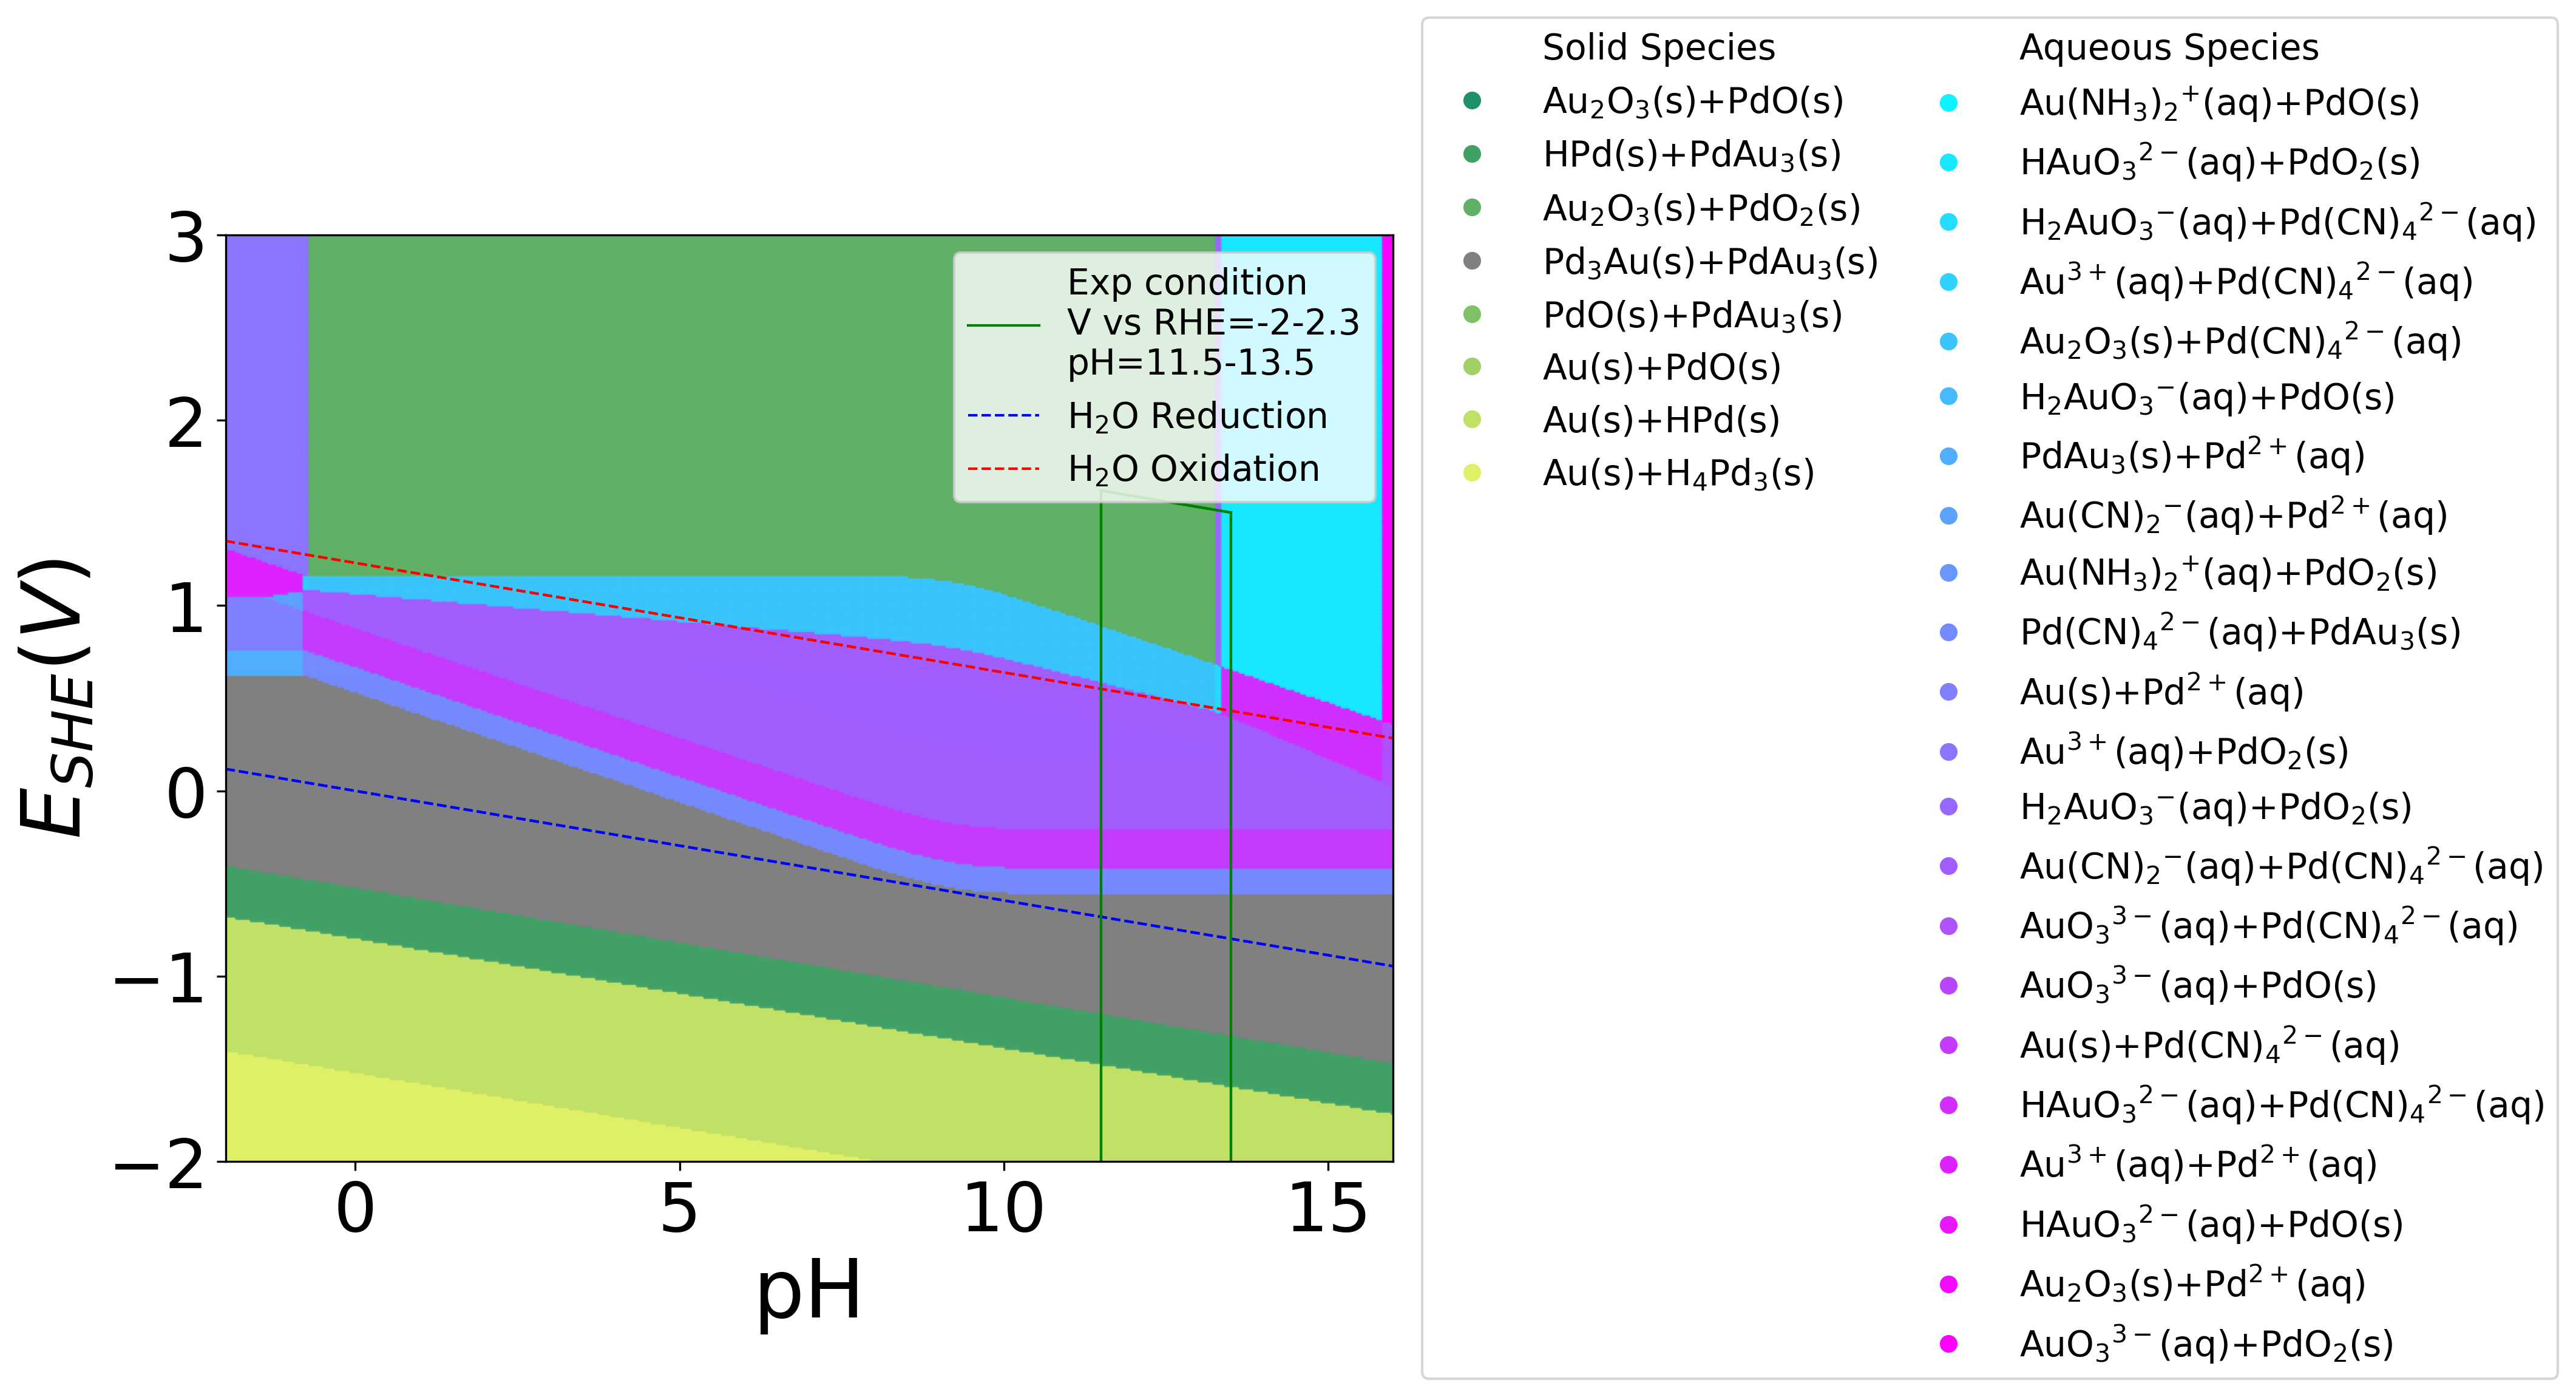
\includegraphics[width=\textwidth]{Figures/alloy_pourbaix_diagrams/Pd_Au_alloy_Pd0.5 Au0.5_NH3=0.02M_Gly=0.005M_CN=0.0001M_activity=1e-04M.png}
       % \par\medskip   
    \end{subfigure}
    \caption{Au-Pd alloy Pourbaix diagrams with $\text{ion activity} = \num{1e-4}$: (a) $[\ce{NH3}]_\text{initial} = 0.02$~M, $[\text{Gly}]_\text{initial} = 0.005$~M; (b) $[\ce{NH3}]_\text{initial} = 0.02$~M, $[\text{Gly}]_\text{initial} = 0.005$~M, and $[\ce{CN^-}]_\text{initial} = \num{1e-4}$~M. A fixed reference stoichiometry of Pd:Au = 1:1 was applied as a compositional constraint when generating the alloy Pourbaix diagrams. The green box highlights the experimentally relevant region, defined by an applied potential of \SIrange{-2}{2}{V} vs. RHE and a pH range of 11.5 to 13.5. Thermodynamically stable alloy regions are shaded in grey.}
    \label{fig:PdAu_alloy_Pourbaix}
\end{figure}

\subsubsection{Pt-Pd Alloy Stability}
As shown in \Cref{fig:PdPt_Pourbaix_NH3_Gly}, the Pt–Pd alloy is predicted to be thermodynamically stable across a wide pH range and within the experimentally relevant potential window. Since both bulk Pd and Pt are resistant to leaching by \ce{NH3} and glycine, the alloy also exhibits greater stability than their corresponding aqueous complexes. However, alloy formation does not significantly shift the stability domains of Pd–cyanide or Pt–cyanide complexes. Notably, Pt–Pd alloys have demonstrated excellent stability under highly acidic conditions during oxygen reduction reactions \cite{Duan2015NanoporousReaction, Koenigsmann2013TailoringSystems}. Nevertheless, these cyanide complexes are stable at oxidative potentials, which can reduce the alloy’s stability in those regions.

%%%%%%%%%%%%%%%%%%%%%%%%%%%%%%%%% PdPt Alloy %%%%%%%%%%%%%%%%%%%%%%%%%%%%%%%%%
\begin{figure}[htbp]
    \centering
    \begin{subfigure}[b]{0.45\textwidth}
        \subcaption{}\label{fig:PdPt_Pourbaix_NH3_Gly}
        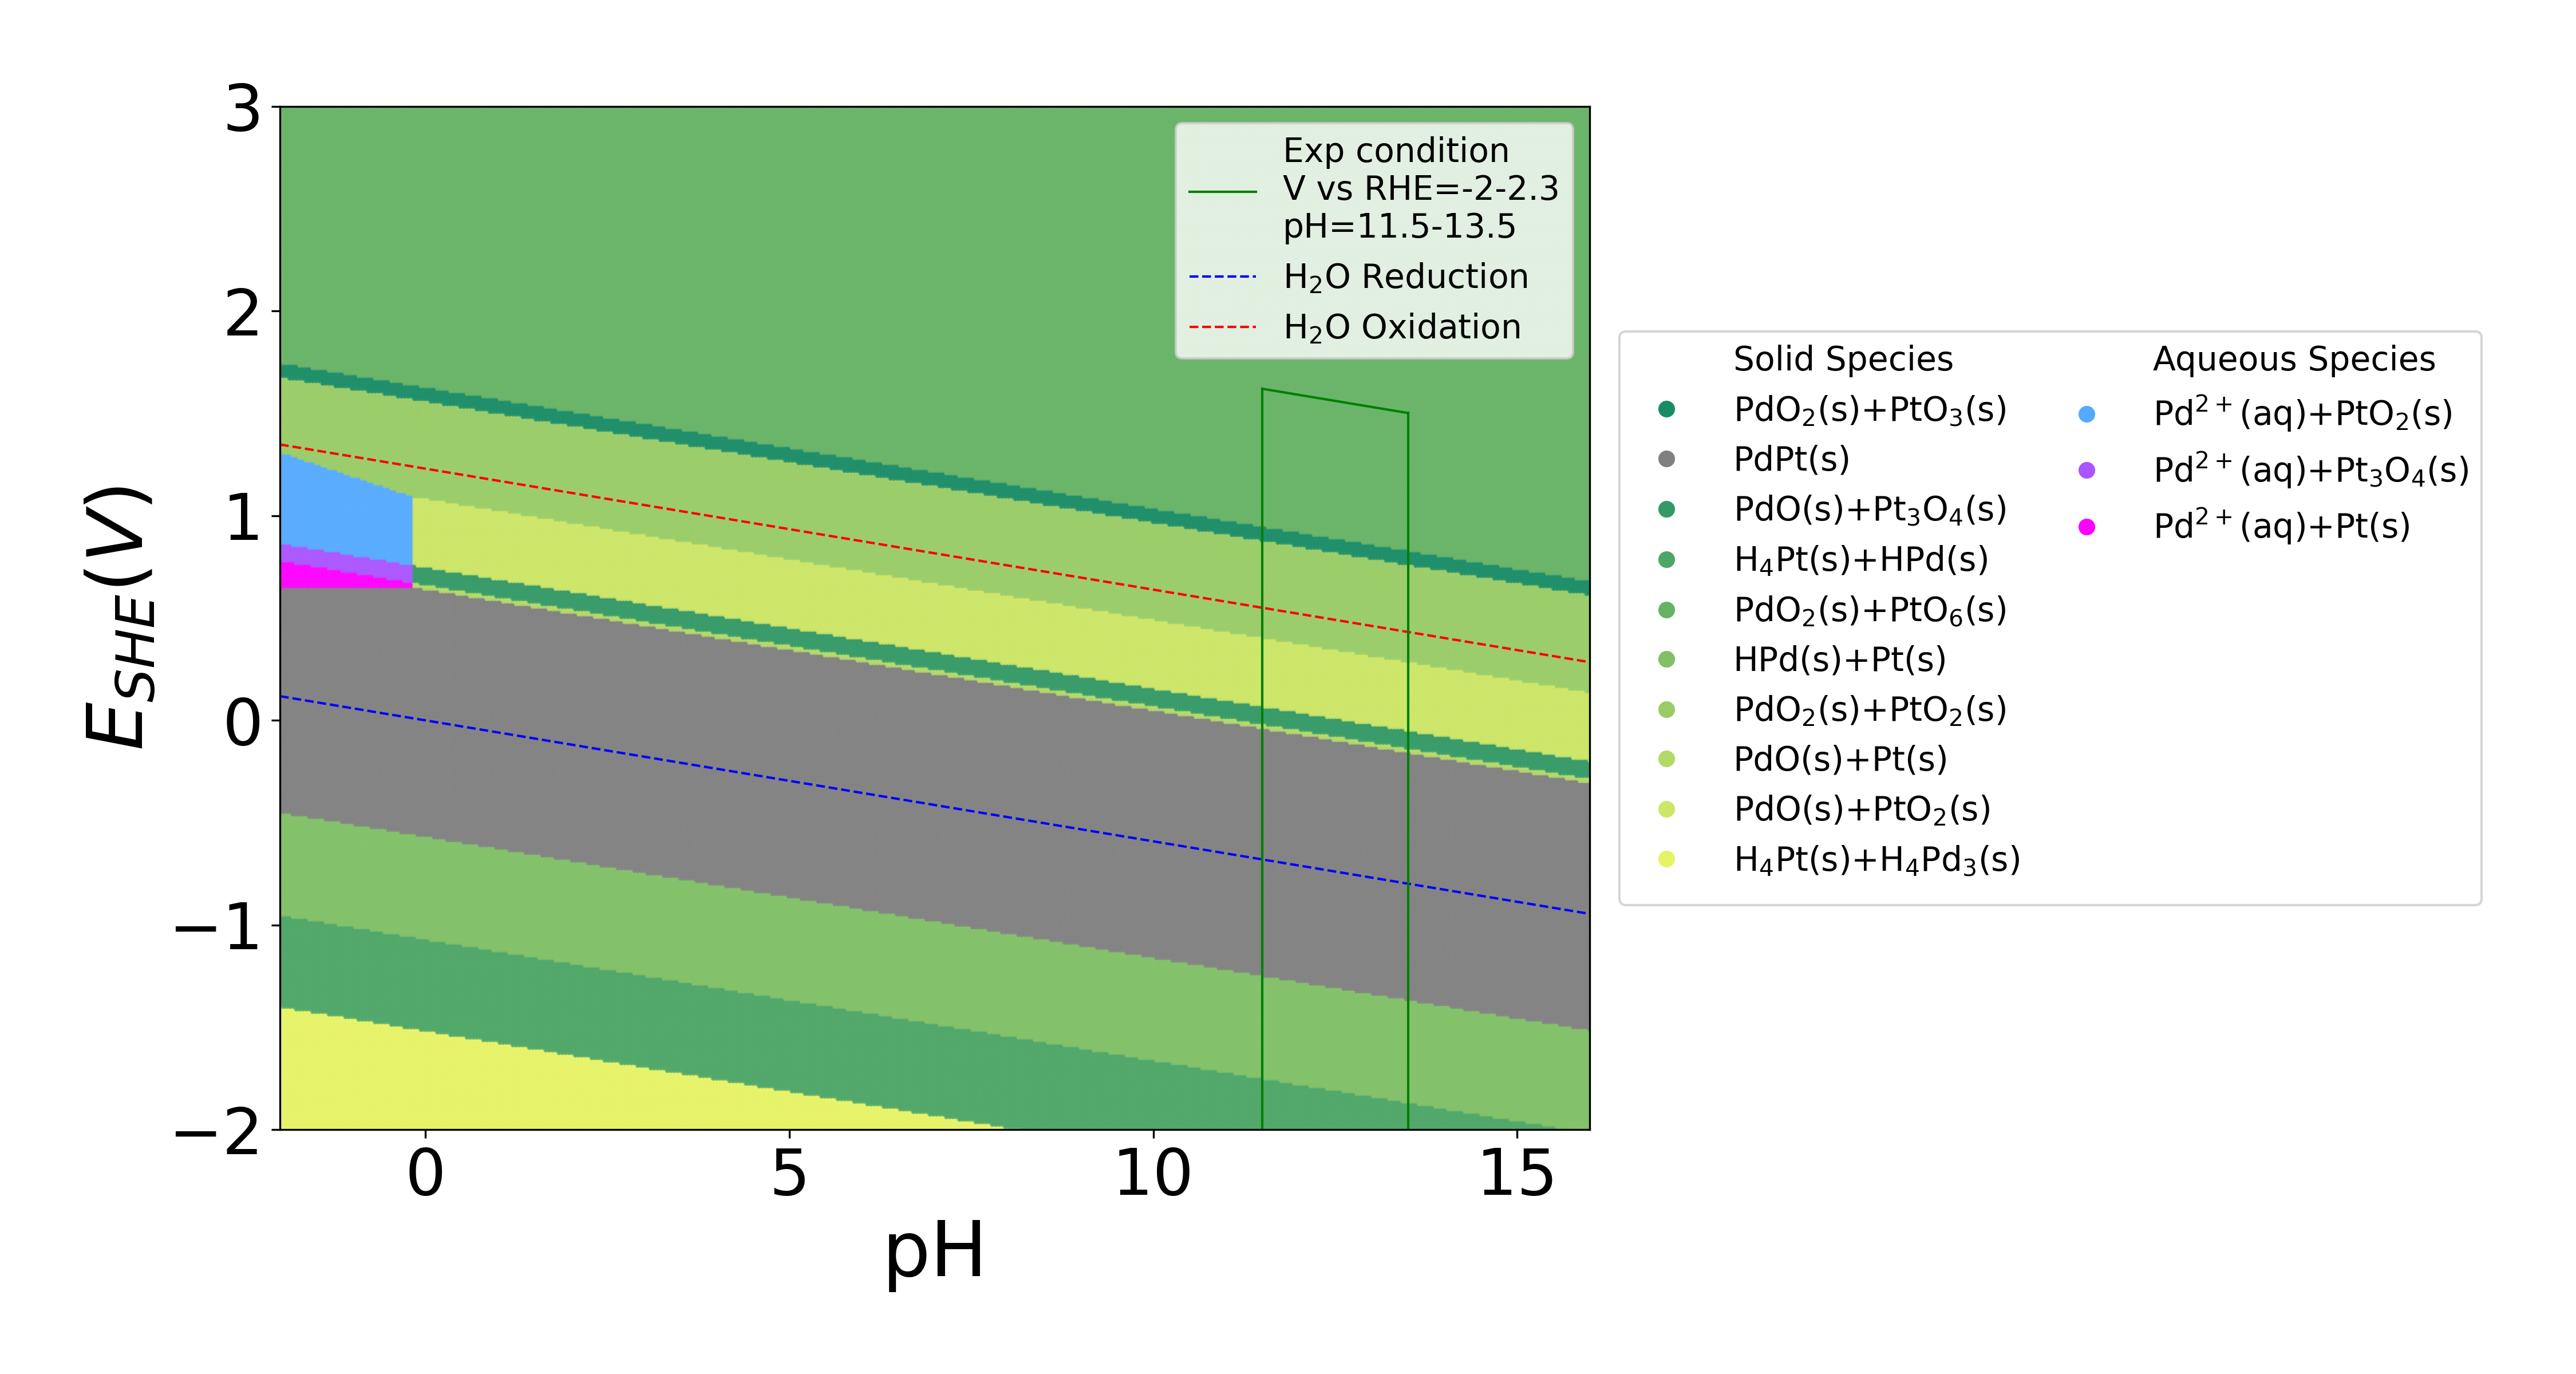
\includegraphics[width=\textwidth]
        {Figures/alloy_pourbaix_diagrams/Pd_Pt_alloy_Pd0.5 Pt0.5_NH3=0.02M_Gly=0.005M_CN=0M_activity=1e-04M.png}
       % \par\medskip
    \end{subfigure}
    \begin{subfigure}[b]{0.45\textwidth}
        \subcaption{}\label{fig:PdPt_Pourbaix_NH3_Gly_CN}
        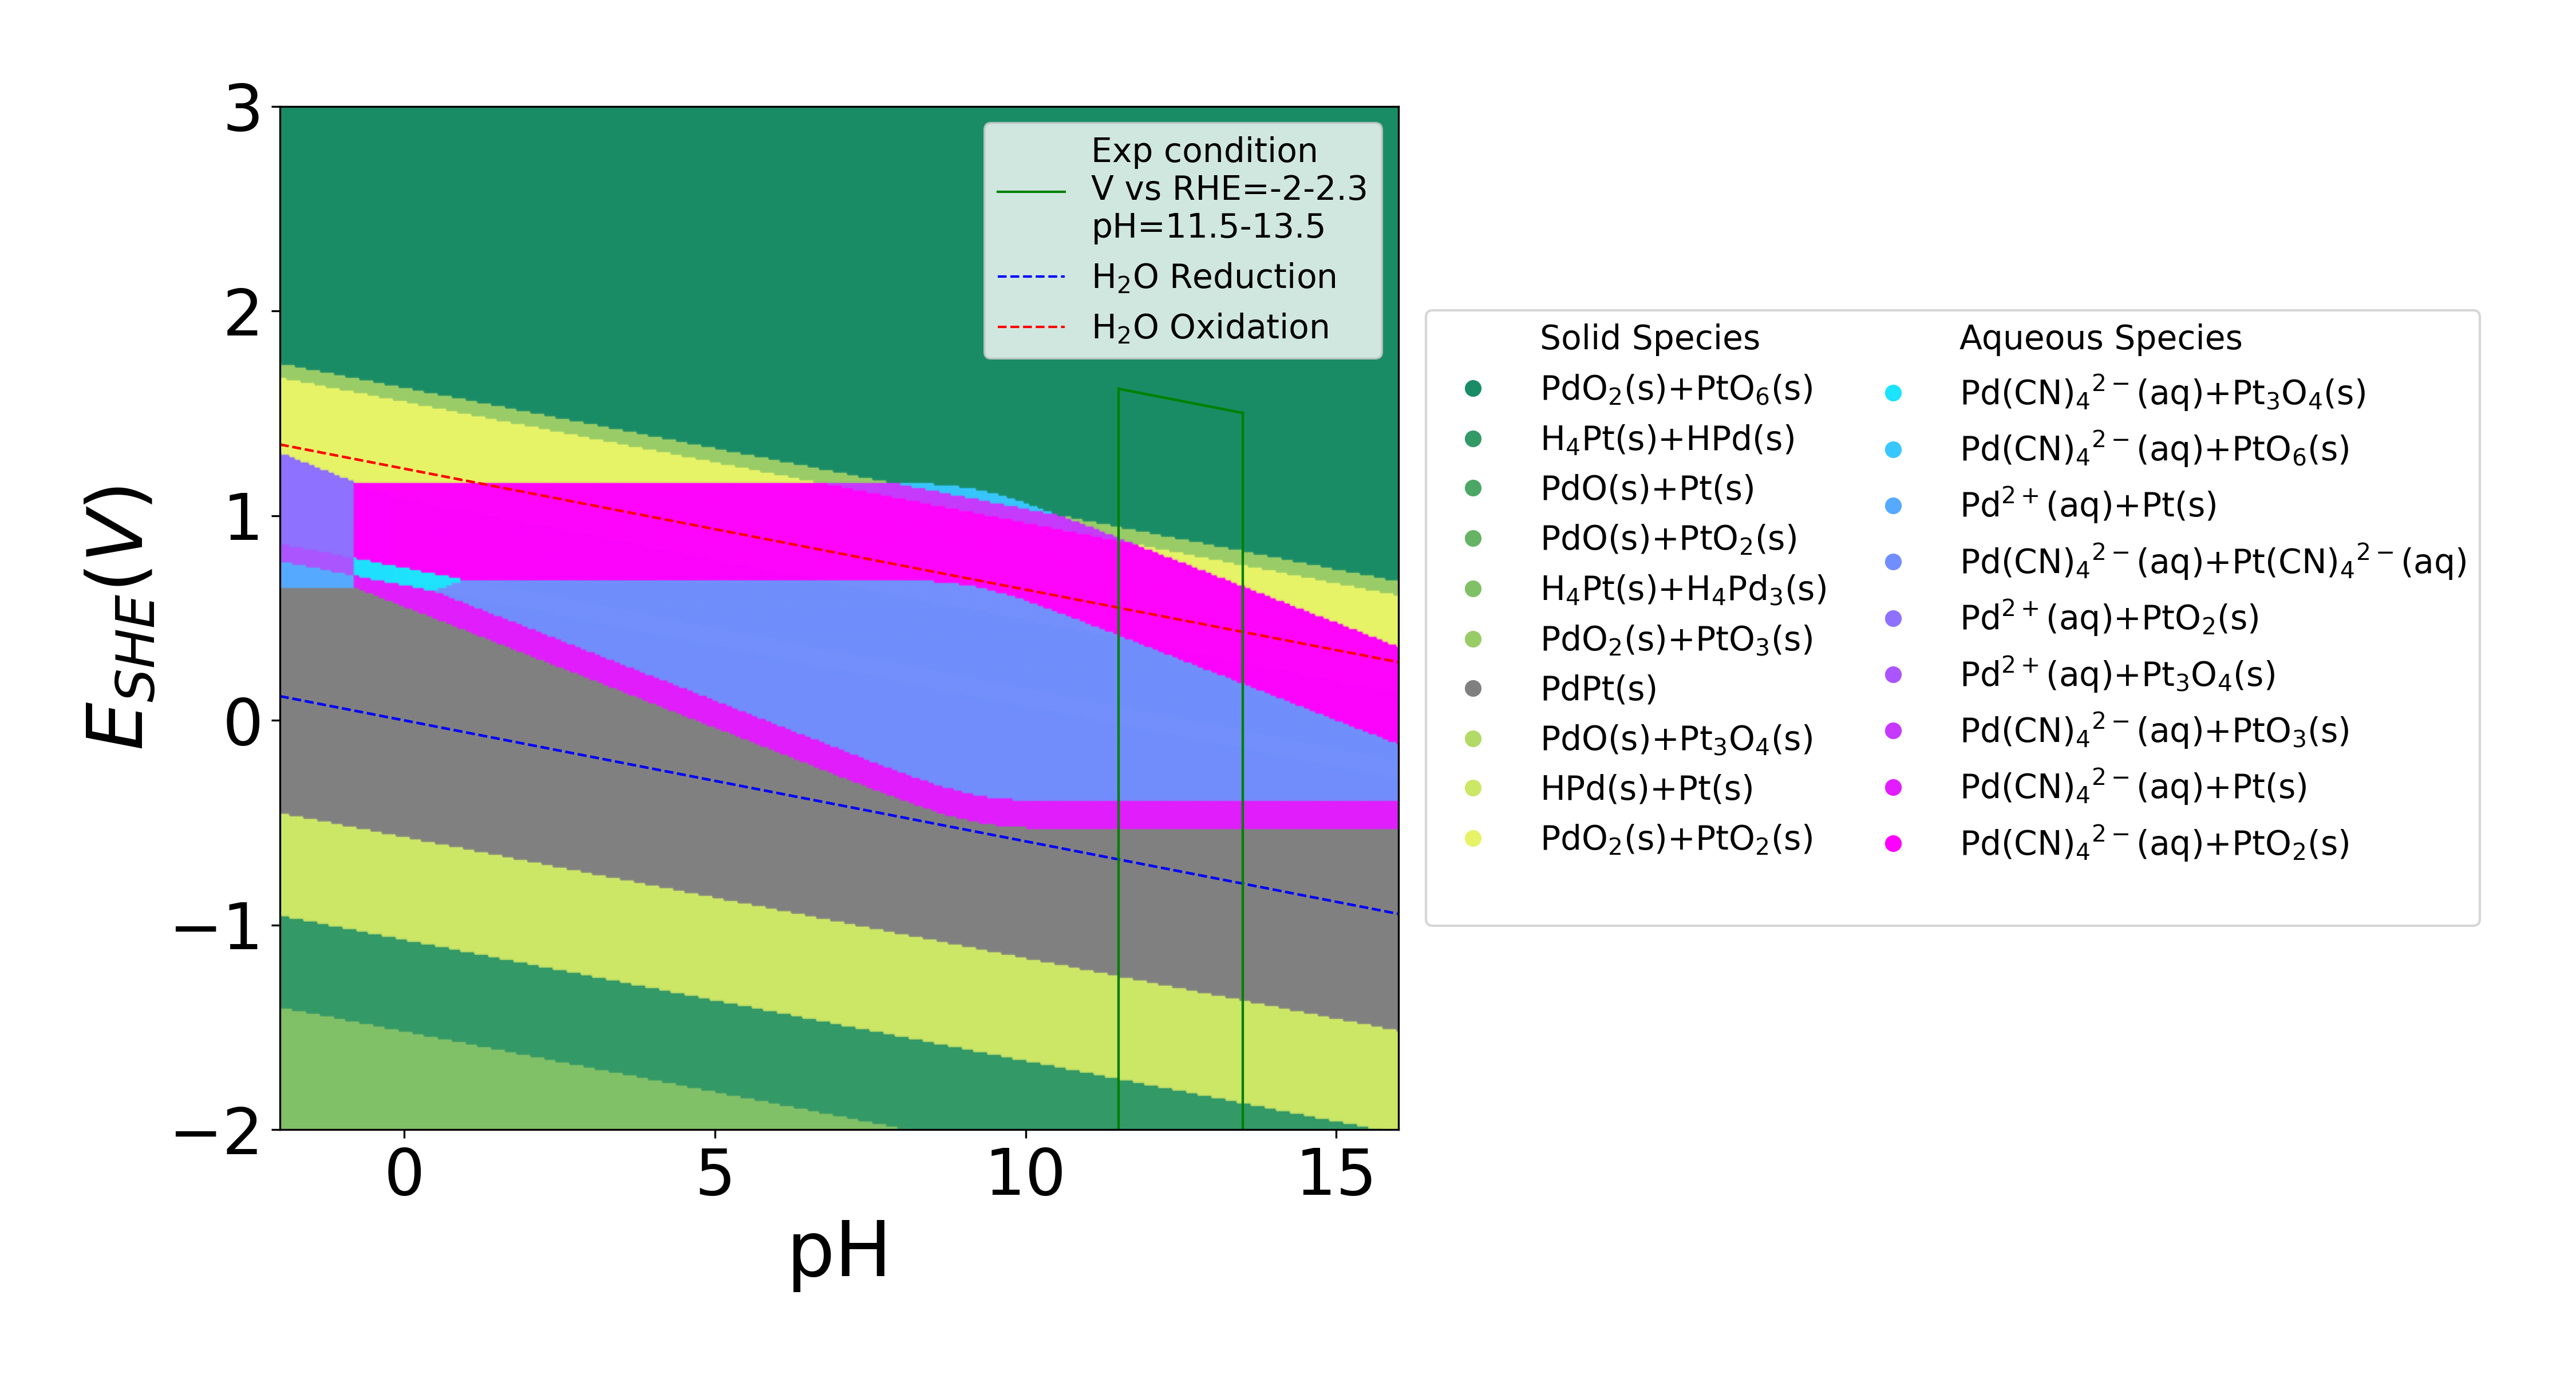
\includegraphics[width=\textwidth]{Figures/alloy_pourbaix_diagrams/Pd_Pt_alloy_Pd0.5 Pt0.5_NH3=0.02M_Gly=0.005M_CN=0.0001M_activity=1e-04M.png}
       % \par\medskip   
    \end{subfigure}
    \caption{Pt-Pd alloy Pourbaix diagrams with $\text{ion activity} = \num{1e-4}$: (a) $[\ce{NH3}]_\text{initial} = 0.02$~M, $[\text{Gly}]_\text{initial} = 0.005$~M; (b) $[\ce{NH3}]_\text{initial} = 0.02$~M, $[\text{Gly}]_\text{initial} = 0.005$~M, and $[\ce{CN^-}]_\text{initial} = \num{1e-4}$~M. A fixed reference stoichiometry of Pd:Pt = 1:1 was applied as a compositional constraint when generating the alloy Pourbaix diagrams. The green box highlights the experimentally relevant region, defined by an applied potential of \SIrange{-2}{2}{V} vs. RHE and a pH range of 11.5 to 13.5. Thermodynamically stable alloy regions are shaded in grey.}
    \label{fig:PdPt_alloy_Pourbaix}
\end{figure}



\subsection{Limitations}
The analysis presented in this study is based on bulk thermodynamic limits, assuming equilibrium behavior among all solid and solution-phase species. While Pourbaix diagrams provide a valuable framework for assessing material stability, they do not account for the non-equilibrium nature of real electrochemical systems, particularly under pulsed potentials catalytic conditions. Real systems often exhibit metastable behavior governed by kinetic barriers to dissolution, phase transformation, or passivation. These kinetic limitations may suppress processes predicted to be thermodynamically favorable.

In addition, the diagrams neglect surface-specific phenomena such as surface reconstruction, segregation, or the formation of solid–electrolyte interphases, all of which can influence stability and activity under operating conditions. Mechanical degradation, cased by lattice mismatch or electrochemical cycling, is also not captured. These factors are especially important for alloys or oxide mixtures, where interfacial stresses and structural mismatches can lead to cracking over time.

The thermodynamic data are derived from DFT calculations using the GGA-PBE functional, which introduces systematic errors in formation energies and redox potentials, typically around $\pm$0.2 eV. These errors can significantly affect the predicted stability of phases, especially for transition metals or less accurately captured systems such as Cu–Ti and Au–Ti alloys. As emphasized by Sun et al. \cite{Sun2024AssessingStudy}, uncertainties in DFT reference states and exchange-correlation functionals can dominate stability predictions. To illustrate this, \Cref{fig:Ni_Pourbaix_noise} shows that randomly perturbing the formation energy of NiO by as little as $\pm$0.067 to 0.2 eV significantly alters its predicted stability window in the Pourbaix diagram.

Our ligand model assumes the presence of selected nitrogen-containing species (e.g., \ce{NH3}, glycine, and \ce{CN^-}) at estimated concentrations based on EWAS experimental conditions. However, these conditions may vary depending on feedstock composition, local pH gradients, and experimental setups. The impact of other possible ligands, such as sulfate or organic degradation products may influence stability boundaries in real-world environments.

Furthermore, metal-ligand complex energies were derived from experimental stability constants, which carry uncertainty due to measurement variability and simplifications in accounting for solvation. Several alloy compositions are taken directly from the Materials Project database and may not have been experimentally synthesized, further contributing to the uncertainty of the modeled species space.

In summary, this work provides a first-principles thermodynamic screening under idealized assumptions. While it offers insights into possible stable materials, experimental validation is essential to assess the practical performance of candidate alloys under EWAS operating conditions.


%%%%%%%%%%%%%%%%%%%%%%%%%%%%%%%%% Ni with Noise %%%%%%%%%%%%%%%%%%%%%%%%%%%%%%%%%
\begin{figure}[htbp]
    \centering
    \begin{subfigure}[b]{0.45\textwidth}
        \subcaption{}\label{fig:Ni_noise_-0.2}
        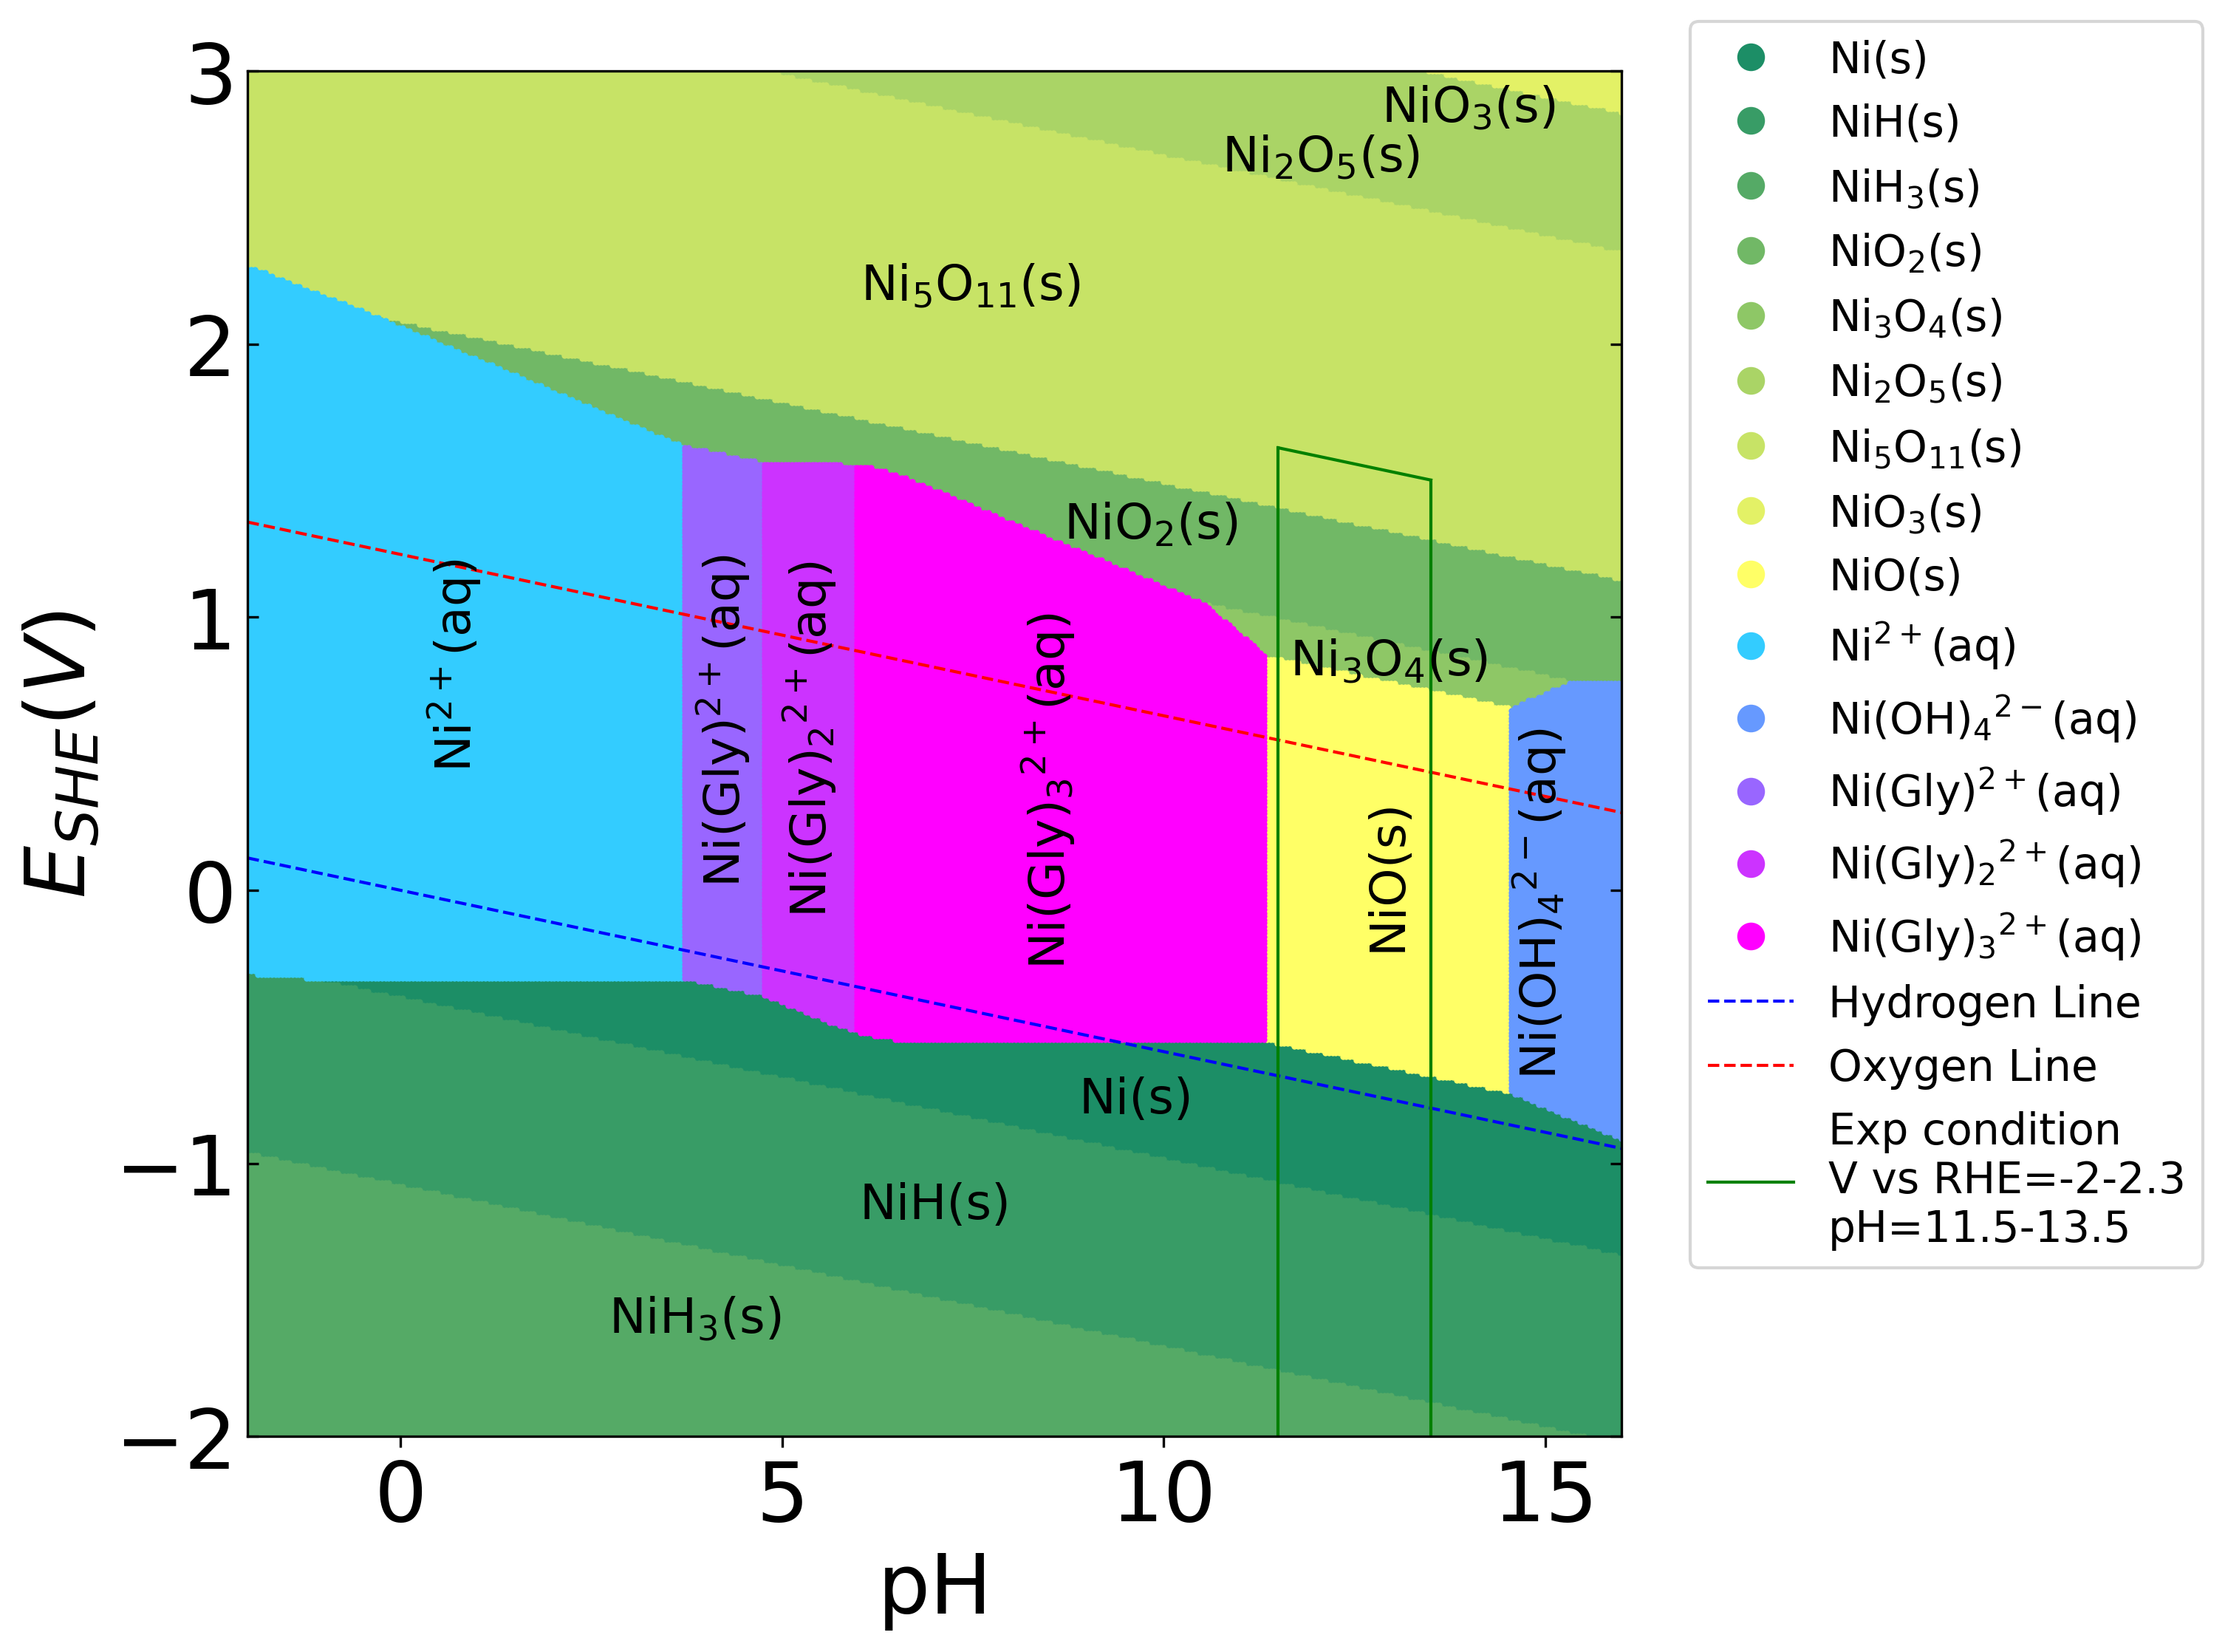
\includegraphics[width=\textwidth]{Figures/pourbaix_diagrams/Ni_gly_-0.2.png}
       % \par\medskip
    \end{subfigure}
    \begin{subfigure}[b]{0.45\textwidth}
        \subcaption{}\label{fig:Ni_noise_-0.067}
        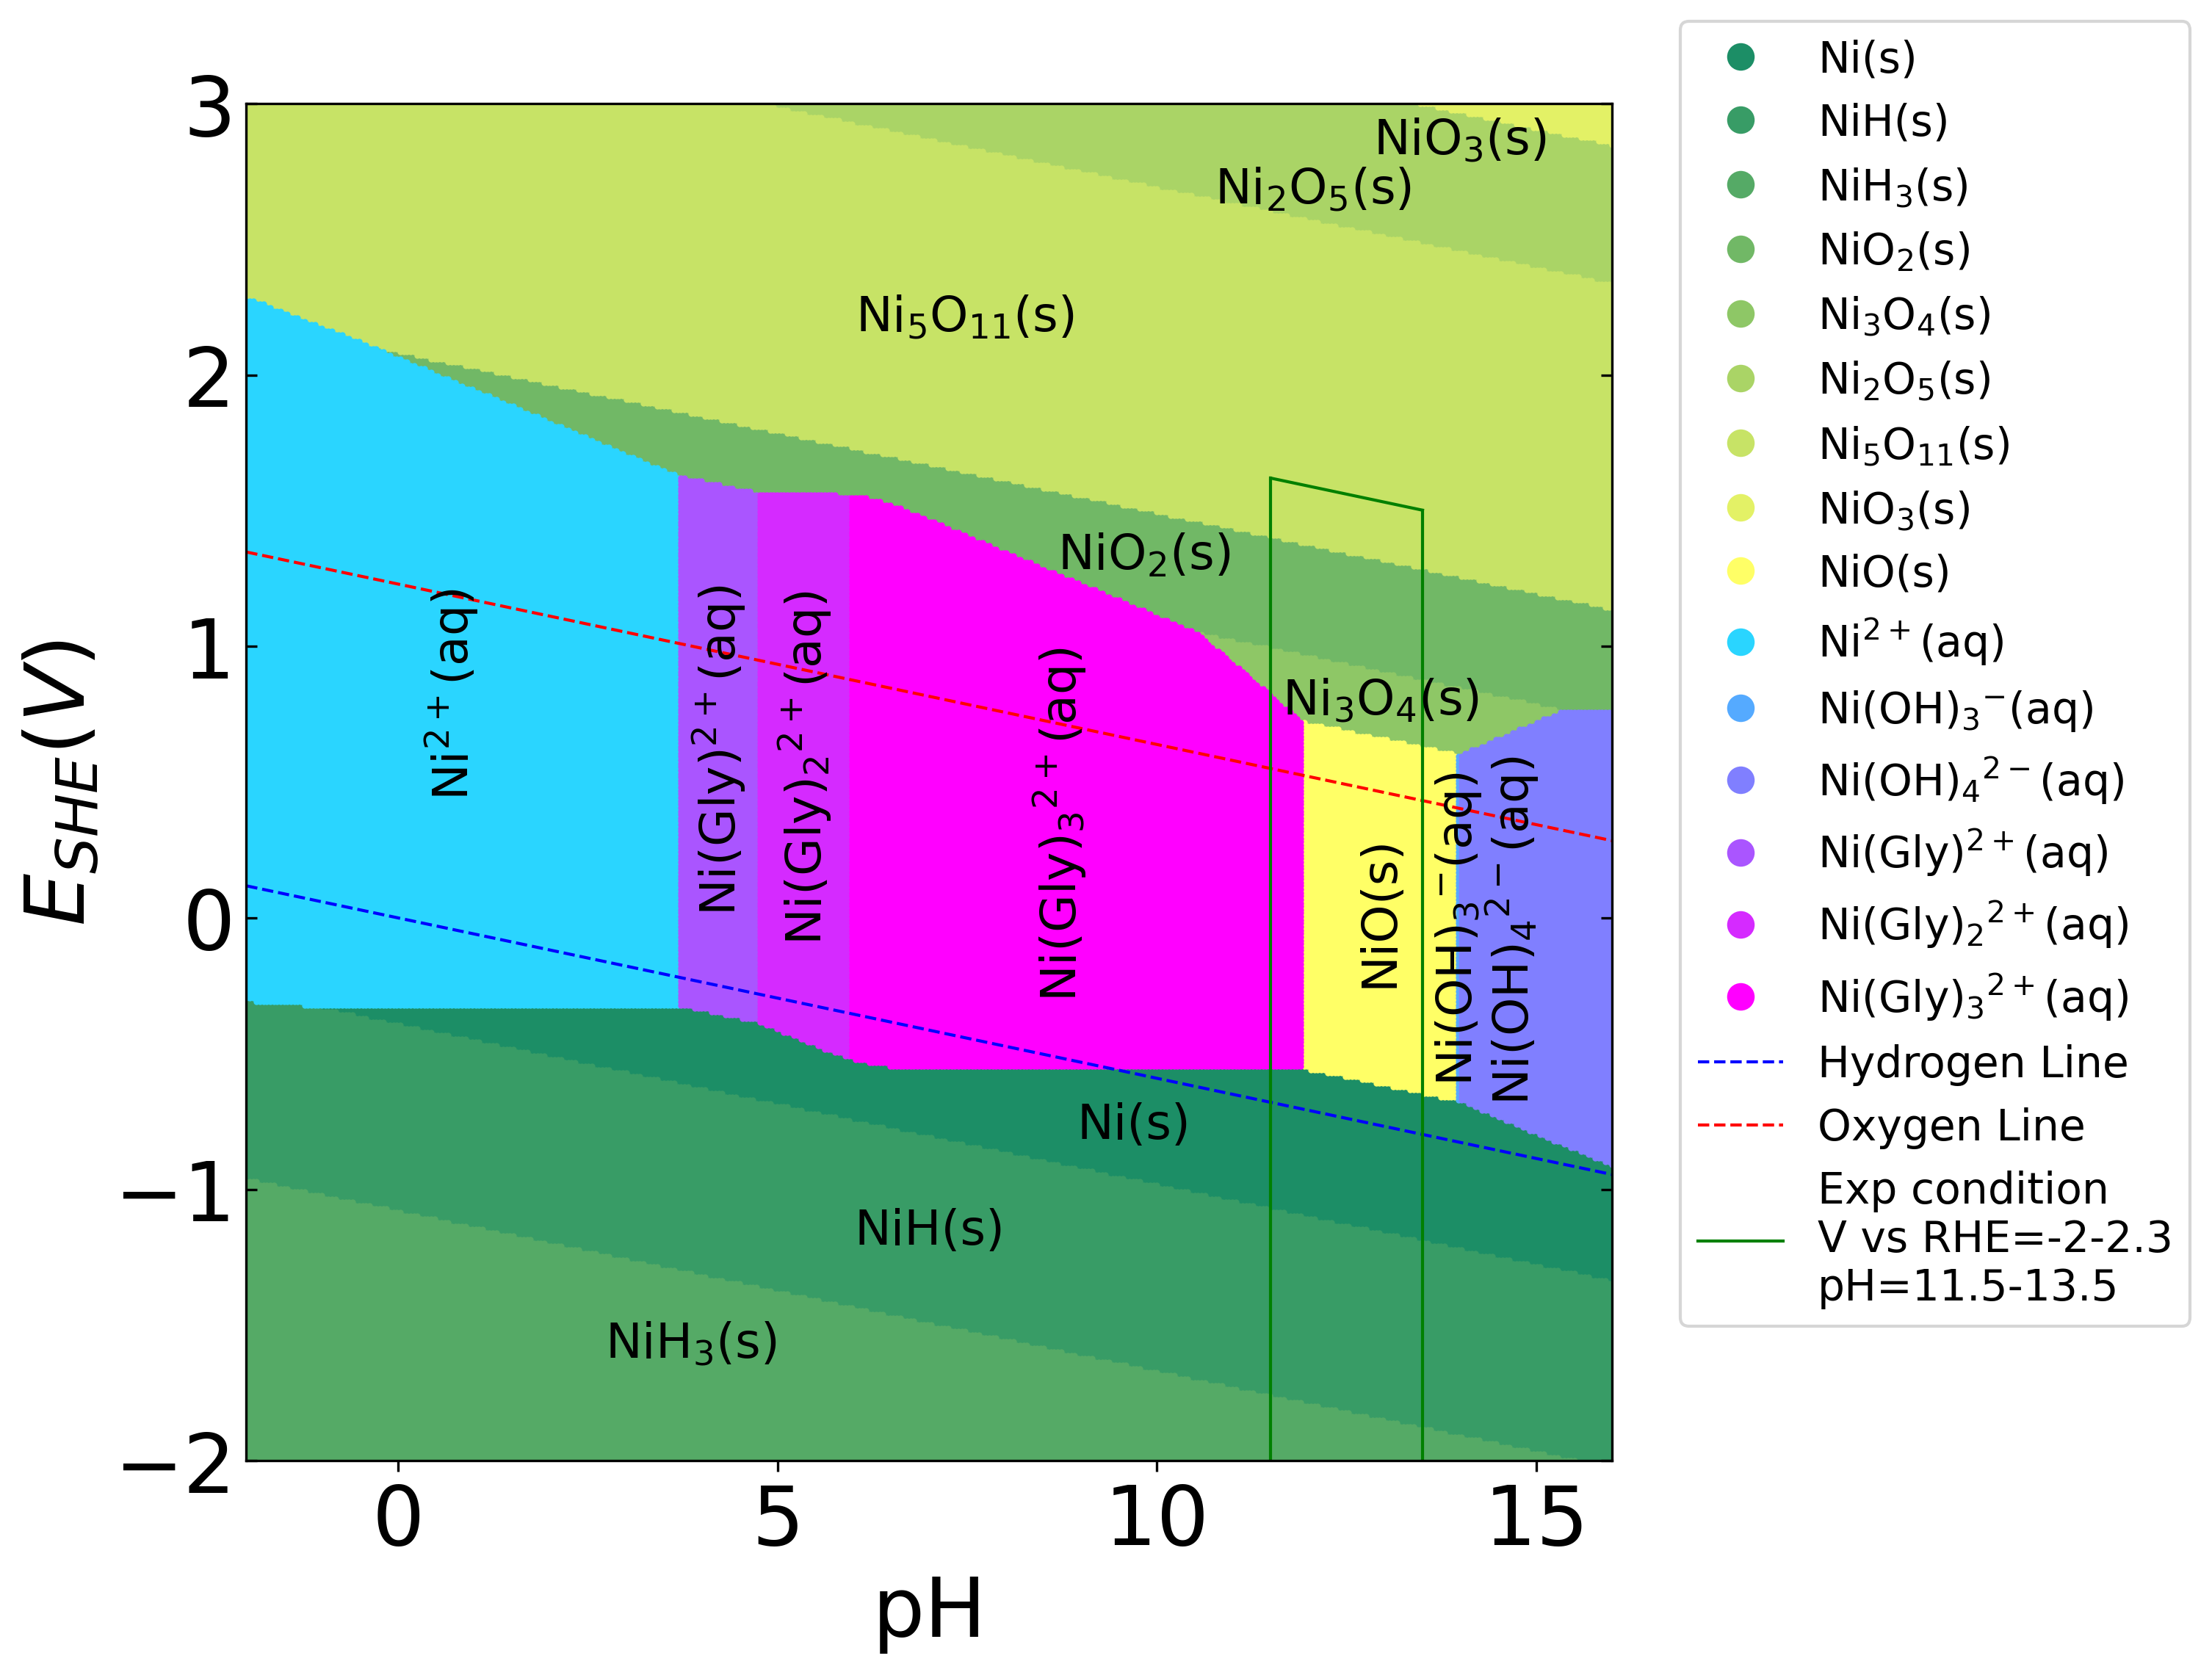
\includegraphics[width=\textwidth]{Figures/pourbaix_diagrams/Ni_gly_-0.06666666666666668.png} 
       % \par\medskip
    \end{subfigure}
    \begin{subfigure}[b]{0.45\textwidth}
        \subcaption{}\label{fig:Ni_noise_0.067}
        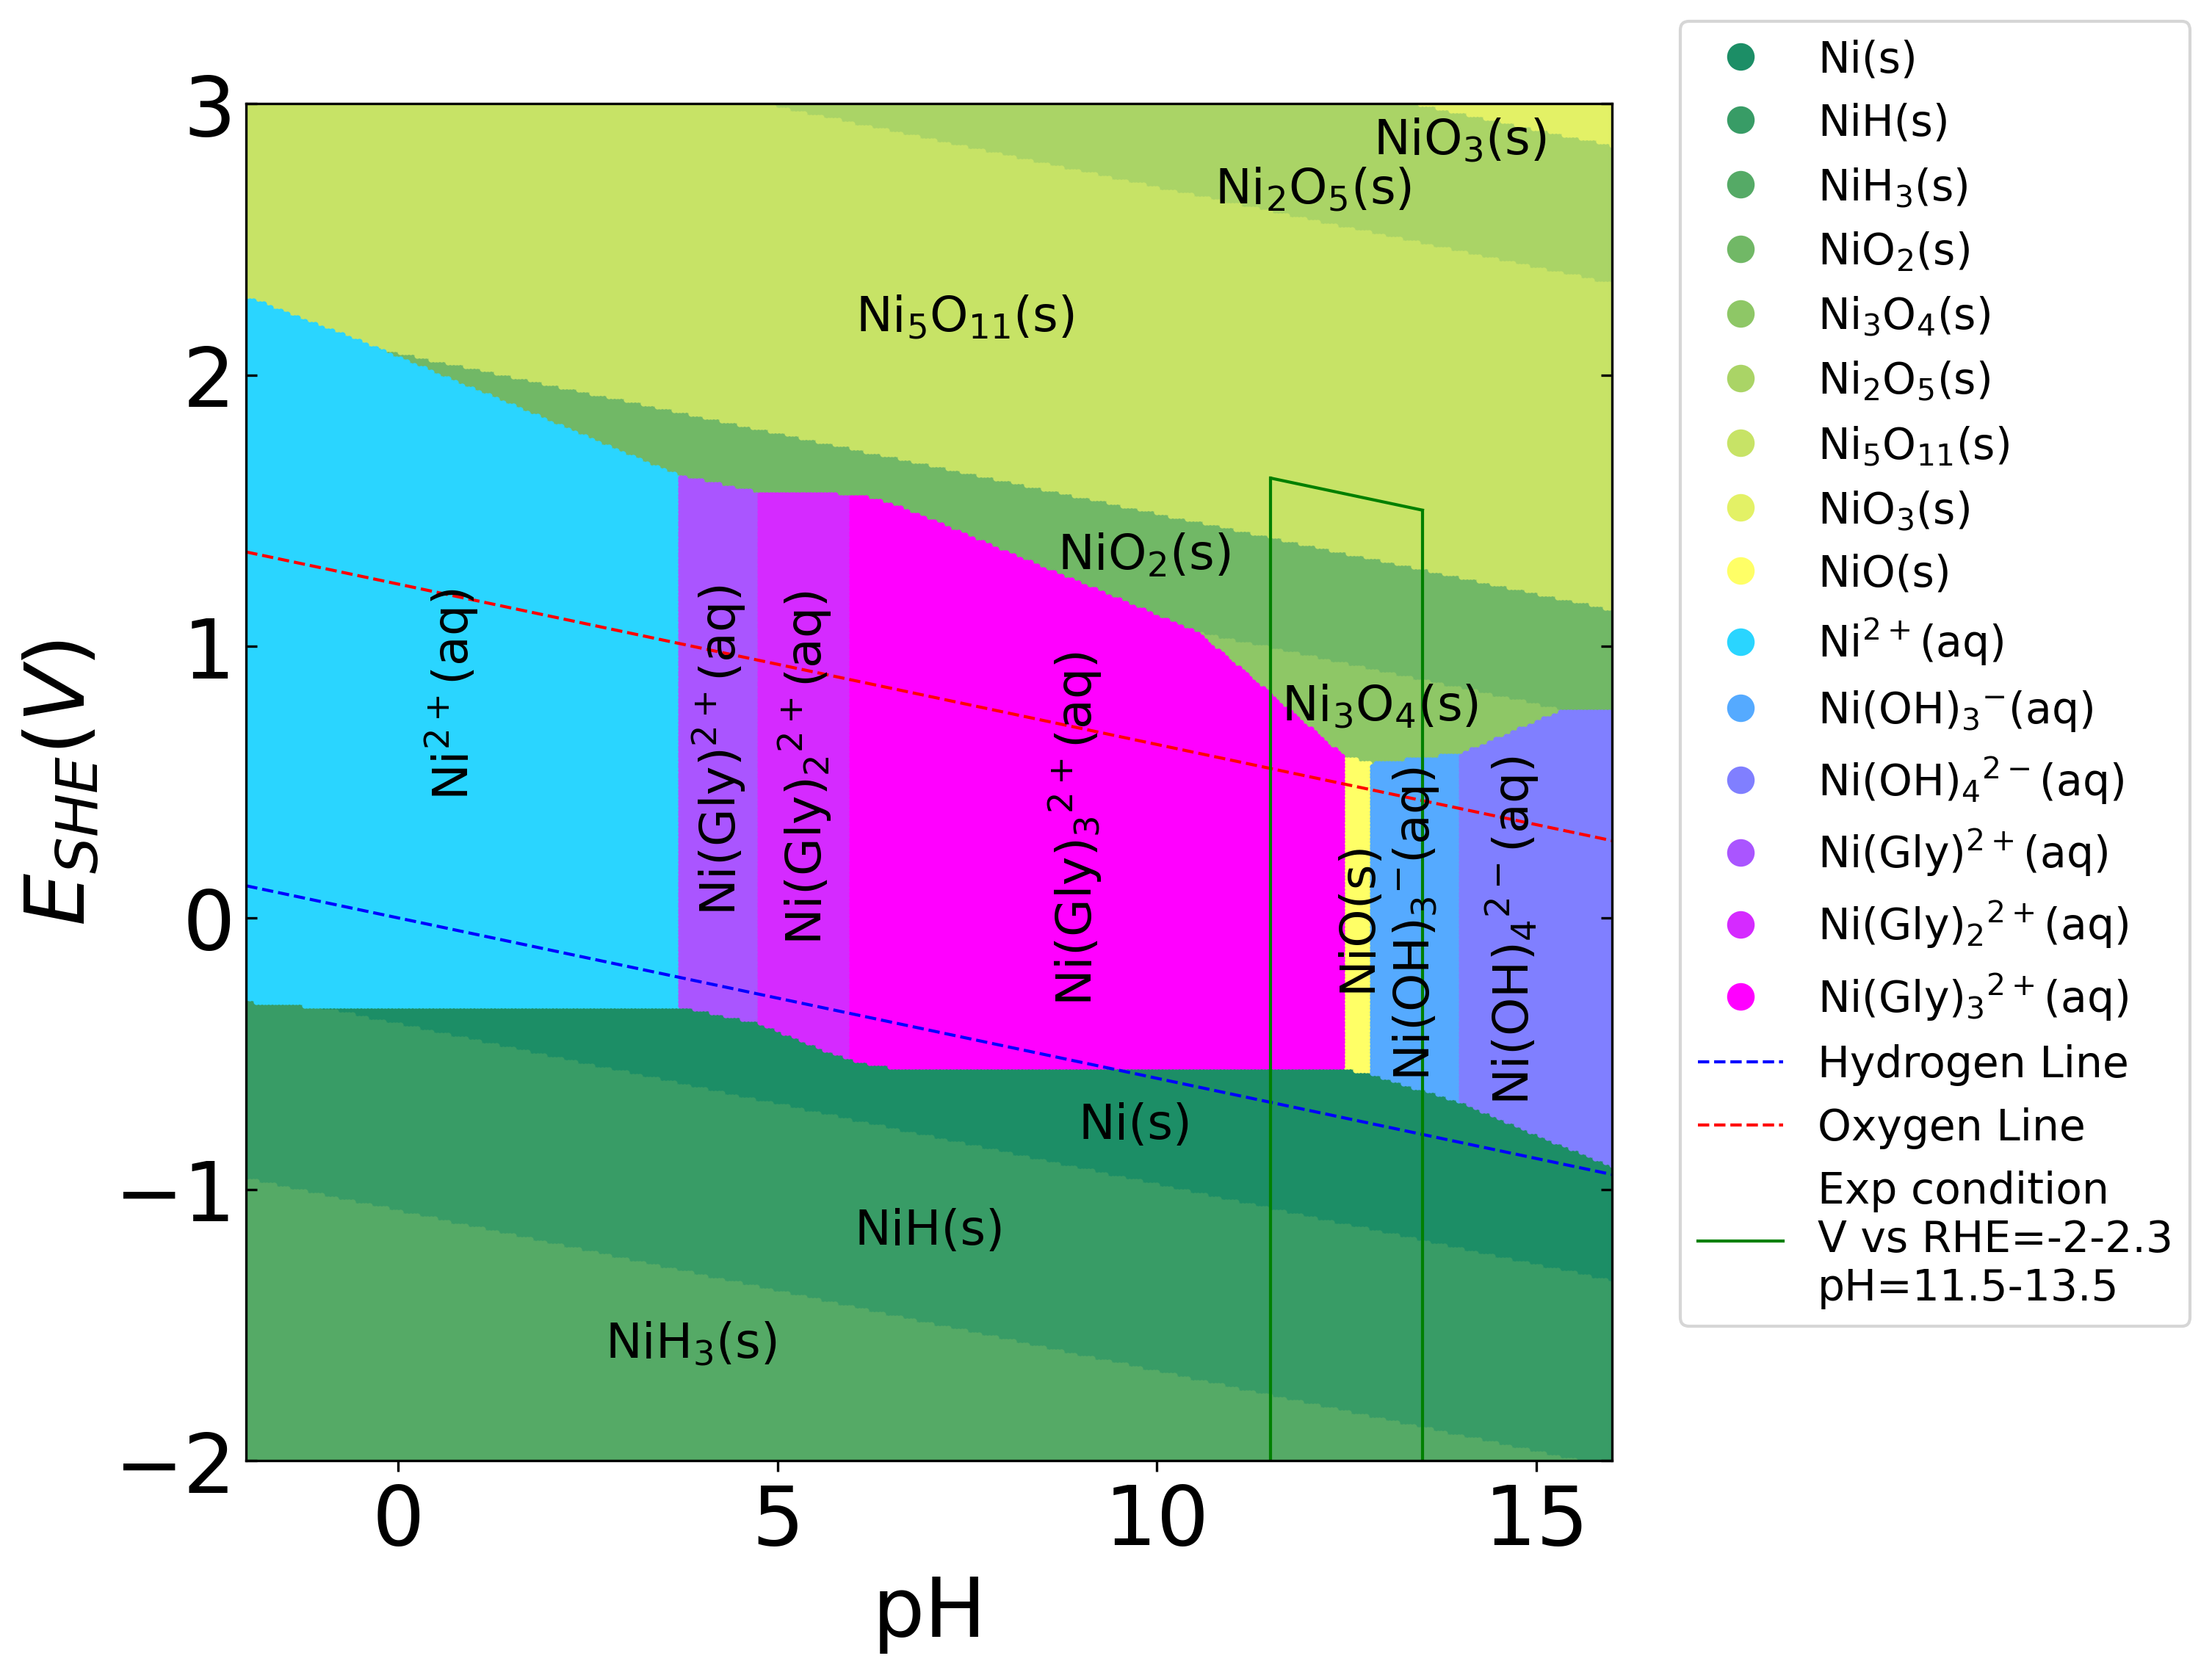
\includegraphics[width=\textwidth]{Figures/pourbaix_diagrams/Ni_gly_0.06666666666666665.png} 
       % \par\medskip   
    \end{subfigure}
    \begin{subfigure}[b]{0.45\textwidth}
        \subcaption{}\label{fig:Ni_noise_0.2}
        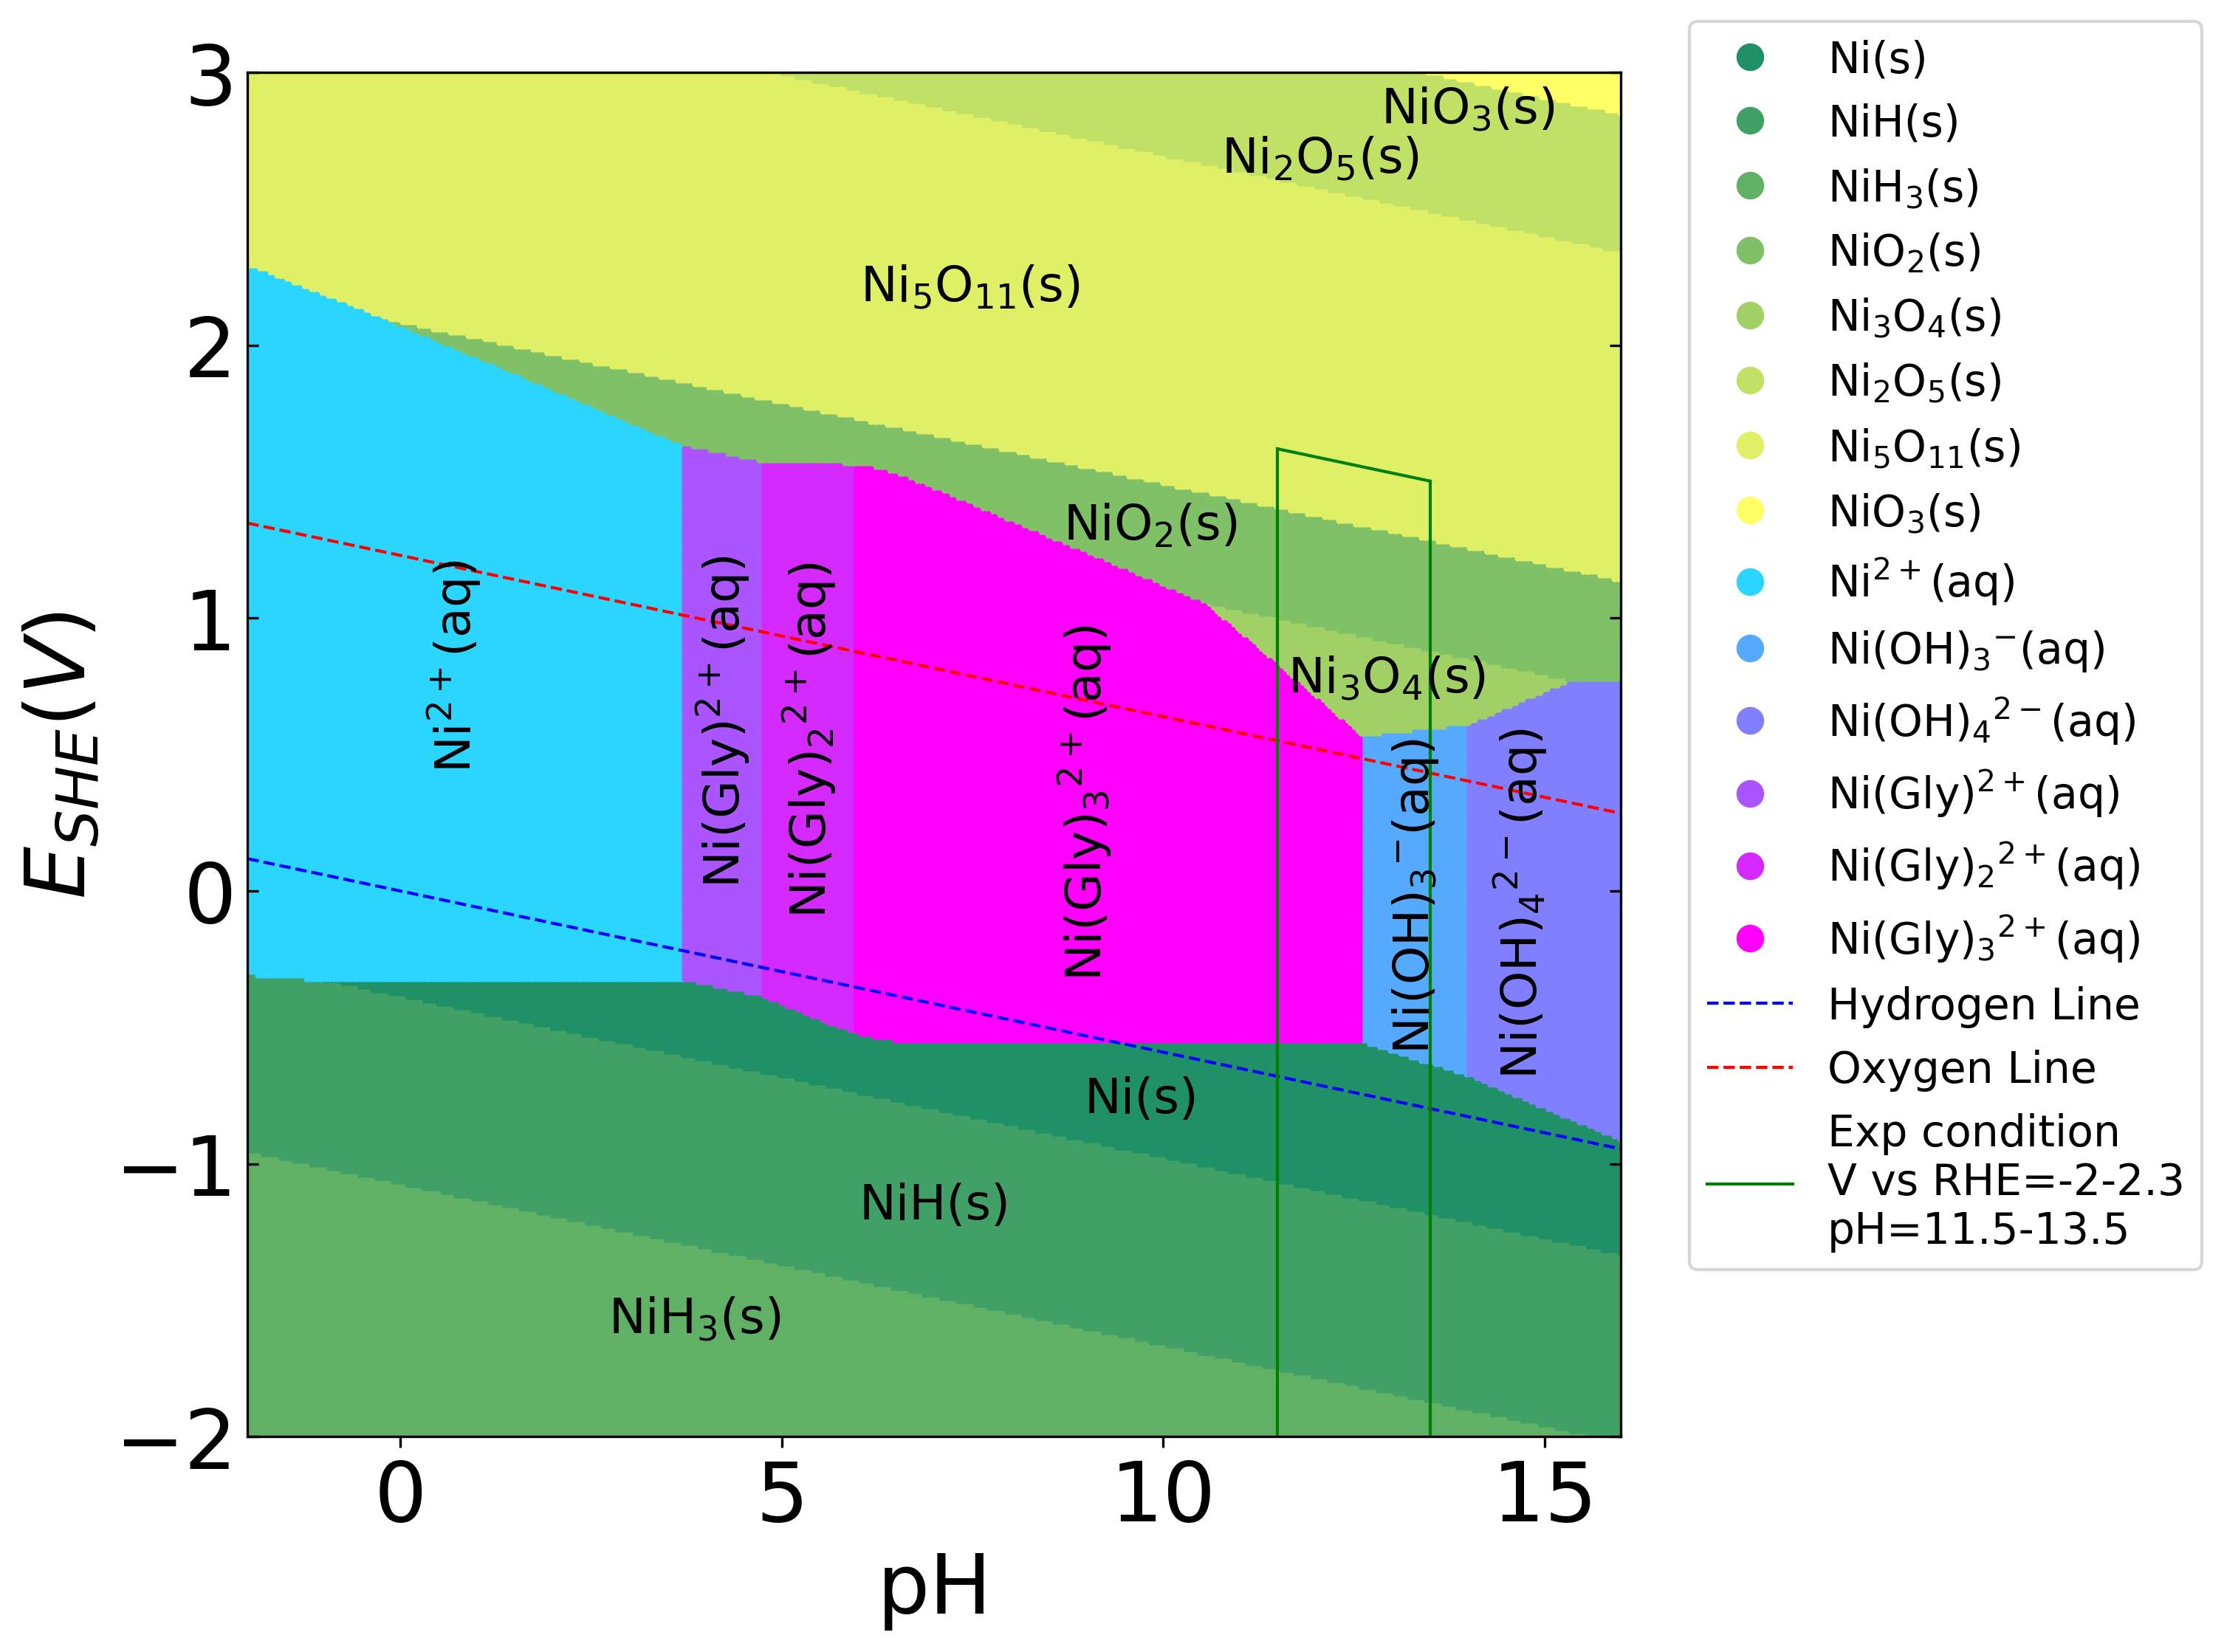
\includegraphics[width=\textwidth]{Figures/pourbaix_diagrams/Ni_gly_0.2.png} 
       % \par\medskip
    \end{subfigure}
    
    \caption{Ni Pourbaix diagrams showing the effect of formation energy perturbations on NiO: (a) $-0.2$ eV, (b) $-0.067$ eV, (c) $+0.067$ eV, and (d) $+0.2$ eV. All diagrams assume ion activity $= \num{1e-4}$ M. The green box highlights experimental conditions: pH = 11.5–13.5 and applied potential vs. RHE = $-2$ to $2$ V.}
    \label{fig:Ni_Pourbaix_noise}
\end{figure}


\section{Conclusion}

This study evaluates the stability of various transitional metal electrodes in EWAS conditions using Pourbaix diagrams, highlighting the critical role of nitrogen-containing ligands in governing corrosion behavior. While Ni and Cu exhibit strong resistance to oxidation in pure aqueous environments, they are highly susceptible to dissolution in the presence of \ce{CN^-} ligands. Pd and Pt are relatively inert toward glycine and ammonia but form stable cyanide complexes even at low concentrations, with inconsistencies in reported stability constants introducing uncertainty in their predicted durability. Given these limitations, alongside their high cost, Pd and Pt are less favorable pure metal candidates for EWAS deployment.

In contrast, Ti demonstrates excellent corrosion resistance across the EWAS-relevant pH and potential range due to its robust passivating oxide layer. However, the \ce{TiO2} layer's poor electronic conductivity may limit catalytic performance unless incorporated into conductive materials such as doped perovskites, MXenes, or metal alloys.

To address this, we explored the stability of Ti-based and Pd-based alloys using Pourbaix diagrams. Alloys such as Ni-Ti and Cu-Ti combine the corrosion resistance of Ti with the catalytic activity or conductivity of the dopant metal. Additionally, Au-Pd and Pt-Pd alloys are investigated for their potential to improve the balance between catalytic activity and stability under redox-dynamic EWAS conditions. These alloying strategies demonstrate that tailored materials design may mitigate the tradeoffs between stability and activity.

Overall, this work emphasizes the importance of integrating thermodynamic screening of both pure and alloyed materials to guide the rational design of EWAS electrodes with enhanced corrosion resistance, minimal leaching, and sustained performance in nitrogen-rich environments.


\section{CRediT authorship contribution statement}
Nianhan Tian: Conceptualization, Methodology, Formal analysis, Software, Visualization, Writing – Original Draft.  \\
Ehsan Abbasi: Investigation, Validation, Writing – Review \& Editing.  \\
Haldrian Iriawan: Investigation, Validation, Writing – Review \& Editing.  \\
Paul Kohl: Resources, Writing – Review \& Editing.  \\
Andrew J. Medford: Conceptualization, Supervision, Project administration, Writing – Review \& Editing.\\


% Pourbaix diagrams of metal-\ce{NH3}/glycine/\ce{CN-}-\ce{H2O} are generated and discussed to identify thermodynamic behavior of an ideal material what can be used as an electrode in EWAS. The dissolvation behavior of various electrode under oxidizing potentials and high N-ligand concentrations was well explained by these pourbaix diagrams. The stability regions of build Ti and it oxides compared with other metals present its thermodynamically stability under such conditions. 
% \subsection{Outline}



\begin{acknowledgement}

% Please use ``The authors thank \ldots'' rather than ``The
% authors would like to thank \ldots''.

% The author thanks Mats Dahlgren for version one of \textsf{achemso},
% and Donald Arseneau for the code taken from \textsf{cite} to move
% citations after punctuation. Many users have provided feedback on the
% class, which is reflected in all of the different demonstrations
% shown in this document.

\end{acknowledgement}

%%%%%%%%%%%%%%%%%%%%%%%%%%%%%%%%%%%%%%%%%%%%%%%%%%%%%%%%%%%%%%%%%%%%%
%% The same is true for Supporting Information, which should use the
%% suppinfo environment.
%%%%%%%%%%%%%%%%%%%%%%%%%%%%%%%%%%%%%%%%%%%%%%%%%%%%%%%%%%%%%%%%%%%%%
\begin{suppinfo}
Free energies of metal-ligand complexes are available.


\end{suppinfo}

% \documentclass[journal=jacsat,manuscript=article,email=false]{achemso}

\usepackage[version=4]{mhchem} % Formula subscripts using \ce{}
\usepackage{esint}
\usepackage{threeparttable}
\usepackage{xr-hyper} % hyperlinks
\usepackage{hyperref} % hyperlinks
\usepackage{cleveref}
\usepackage{fancyhdr}
\usepackage[numbers]{natbib}
% To number sections, pages, figures and tables nested within chapters:
% \renewcommand{\thepage}{\arabic{chapter}.\arabic{page}} 
% \renewcommand{\thesection}{\arabic{chapter}.\arabic{section}}  
% \renewcommand{\thetable}{\arabic{chapter}.\arabic{table}}  
% \renewcommand{\thefigure}{\arabic{chapter}.\arabic{figure}}

% To number supplemental material with 'S':
% \renewcommand{\thepage}{S\arabic{page}} 
\renewcommand{\thesection}{S\arabic{section}}  
\renewcommand{\thetable}{S\arabic{table}}  
\renewcommand{\thefigure}{S\arabic{figure}}
\renewcommand{\theequation}{S\arabic{equation}}

\usepackage{longtable} % For multi-page tables
\usepackage{array}

\pagestyle{fancy}
\fancyhf{}
\cfoot{S\thepage}
\renewcommand{\headrulewidth}{0pt}


\author{Nianhan Tian}
\affiliation[Georgia Institute of Technology]
{School of Chemical and Biomolecular Engineering, Georgia Institute of Technology, Atlanta, Georgia 30318 USA}

\author{Andrew J. Medford}
\affiliation[Georgia Institute of Technology]
{School of Chemical and Biomolecular Engineering, Georgia Institute of Technology, Atlanta, Georgia 30318 USA}
\email{ajm@gatech.edu}

\title{Accelerated Computational Materials Discovery for Electrochemical Nutrient Recovery\\\vspace{8pt}\large{Supporting Information}}


\begin{document}
\newpage
\clearpage
\begin{longtable}{|p{4cm}|p{4cm}|p{3cm}|p{3cm}|}
\caption{Formation energies of species for \ce{NH3} complexes.} 
\label{tab:NH3_complex_energies}
\\
\hline
\textbf{Species} & \textbf{Metal ion} & \textbf{\( \Delta G^\circ_{298} \) (eV)} & \textbf{Reference} \\ \hline
\endfirsthead
\caption*{Table \thetable\ continued from previous pages.} \\
\hline
\textbf{Species} & \textbf{Metal ion} & \textbf{\( \Delta G^\circ_{298} \) (eV)} & \textbf{Reference} \\ \hline
\endhead
\hline
\endfoot
\hline
\endlastfoot
\ce{[Ag.0(NH3).0].0+} & \ce{Ag^1+} & 0.322 & \textnormal{\citenum{Bjerrum1957StabilitySubstances}} \\ \hline
\ce{[Ag.0(NH3)2.0].0+} & \ce{Ag^1+} & -0.191 & \textnormal{\citenum{Bjerrum1957StabilitySubstances}} \\ \hline
\ce{[Au.0(NH3)2.0].0+} & \ce{Au^1+} & -0.325 & \textnormal{\citenum{Bjerrum1957StabilitySubstances}} \\ \hline
\ce{[Au.0(NH3)4.0]^3.0+} & \ce{Au^3+} & 1.681 & \textnormal{\citenum{Bjerrum1957StabilitySubstances}} \\ \hline
\ce{[Ca.0(NH3).0]^2.0+} & \ce{Ca^2+} & -6.001 & \textnormal{\citenum{Bjerrum1957StabilitySubstances}} \\ \hline
\ce{[Ca.0(NH3)2.0]^2.0+} & \ce{Ca^2+} & -6.242 & \textnormal{\citenum{Bjerrum1957StabilitySubstances}} \\ \hline
\ce{[Ca.0(NH3)3.0]^2.0+} & \ce{Ca^2+} & -6.470 & \textnormal{\citenum{Bjerrum1957StabilitySubstances}} \\ \hline
\ce{[Ca.0(NH3)4.0]^2.0+} & \ce{Ca^2+} & -7.001 & \textnormal{\citenum{Bjerrum1957StabilitySubstances}} \\ \hline
\ce{[Cd.0(NH3).0]^2.0+} & \ce{Cd^2+} & -1.234 & \textnormal{\citenum{Bjerrum1957StabilitySubstances}} \\ \hline
\ce{[Cd.0(NH3)2.0]^2.0+} & \ce{Cd^2+} & -1.632 & \textnormal{\citenum{Bjerrum1957StabilitySubstances}} \\ \hline
\ce{[Cd.0(NH3)3.0]^2.0+} & \ce{Cd^2+} & -1.990 & \textnormal{\citenum{Bjerrum1957StabilitySubstances}} \\ \hline
\ce{[Cd.0(NH3)4.0]^2.0+} & \ce{Cd^2+} & -2.318 & \textnormal{\citenum{Bjerrum1957StabilitySubstances}} \\ \hline
\ce{[Cd.0(NH3)5.0]^2.0+} & \ce{Cd^2+} & -2.575 & \textnormal{\citenum{Bjerrum1957StabilitySubstances}} \\ \hline
\ce{[Cd.0(NH3)6.0]^2.0+} & \ce{Cd^2+} & -2.750 & \textnormal{\citenum{Bjerrum1957StabilitySubstances}} \\ \hline
\ce{[Co.0(NH3).0]^2.0+} & \ce{Co^2+} & -0.961 & \textnormal{\citenum{Bjerrum1957StabilitySubstances}} \\ \hline
\ce{[Co.0(NH3)2.0]^2.0+} & \ce{Co^2+} & -1.330 & \textnormal{\citenum{Bjerrum1957StabilitySubstances}} \\ \hline
\ce{[Co.0(NH3)3.0]^2.0+} & \ce{Co^2+} & -1.665 & \textnormal{\citenum{Bjerrum1957StabilitySubstances}} \\ \hline
\ce{[Co.0(NH3)4.0]^2.0+} & \ce{Co^2+} & -1.982 & \textnormal{\citenum{Bjerrum1957StabilitySubstances}} \\ \hline
\ce{[Co.0(NH3)5.0]^2.0+} & \ce{Co^2+} & -2.260 & \textnormal{\citenum{Bjerrum1957StabilitySubstances}} \\ \hline
\ce{[Co.0(NH3)6.0]^2.0+} & \ce{Co^2+} & -2.501 & \textnormal{\citenum{Bjerrum1957StabilitySubstances}} \\ \hline
\ce{[Co.0(NH3).0]^3.0+} & \ce{Co^3+} & 0.681 & \textnormal{\citenum{Bjerrum1957StabilitySubstances}} \\ \hline
\ce{[Co.0(NH3)2.0]^3.0+} & \ce{Co^3+} & 0.008 & \textnormal{\citenum{Bjerrum1957StabilitySubstances}} \\ \hline
\ce{[Co.0(NH3)3.0]^3.0+} & \ce{Co^3+} & -0.628 & \textnormal{\citenum{Bjerrum1957StabilitySubstances}} \\ \hline
\ce{[Co.0(NH3)4.0]^3.0+} & \ce{Co^3+} & -1.236 & \textnormal{\citenum{Bjerrum1957StabilitySubstances}} \\ \hline
\ce{[Co.0(NH3)5.0]^3.0+} & \ce{Co^3+} & -1.814 & \textnormal{\citenum{Bjerrum1957StabilitySubstances}} \\ \hline
\ce{[Co.0(NH3)6.0]^3.0+} & \ce{Co^3+} & -2.350 & \textnormal{\citenum{Bjerrum1957StabilitySubstances}} \\ \hline
\ce{[Cu.0(NH3).0].0+} & \ce{Cu^1+} & -0.107 & \textnormal{\citenum{Bjerrum1957StabilitySubstances}} \\ \hline
\ce{[Cu.0(NH3)2.0].0+} & \ce{Cu^1+} & -0.673 & \textnormal{\citenum{Bjerrum1957StabilitySubstances}} \\ \hline
\ce{[Cu.0(NH3).0]^2.0+} & \ce{Cu^2+} & 0.158 & \textnormal{\citenum{Bjerrum1957StabilitySubstances}} \\ \hline
\ce{[Cu.0(NH3)2.0]^2.0+} & \ce{Cu^2+} & -0.324 & \textnormal{\citenum{Bjerrum1957StabilitySubstances}} \\ \hline
\ce{[Cu.0(NH3)3.0]^2.0+} & \ce{Cu^2+} & -0.769 & \textnormal{\citenum{Bjerrum1957StabilitySubstances}} \\ \hline
\ce{[Cu.0(NH3)4.0]^2.0+} & \ce{Cu^2+} & -1.170 & \textnormal{\citenum{Bjerrum1957StabilitySubstances}} \\ \hline
\ce{[Fe.0(NH3).0]^2.0+} & \ce{Fe^2+} & -1.177 & \textnormal{\citenum{Bjerrum1957StabilitySubstances}} \\ \hline
\ce{[Fe.0(NH3)2.0]^2.0+} & \ce{Fe^2+} & -1.500 & \textnormal{\citenum{Bjerrum1957StabilitySubstances}} \\ \hline
\ce{[Fe.0(NH3)4.0]^2.0+} & \ce{Fe^2+} & -2.141 & \textnormal{\citenum{Bjerrum1957StabilitySubstances}} \\ \hline
\ce{[Ni.0(NH3).0]^2.0+} & \ce{Ni^2+} & -0.920 & \textnormal{\citenum{Bjerrum1957StabilitySubstances}} \\ \hline
\ce{[Ni.0(NH3)2.0]^2.0+} & \ce{Ni^2+} & -1.326 & \textnormal{\citenum{Bjerrum1957StabilitySubstances}} \\ \hline
\ce{[Ni.0(NH3)3.0]^2.0+} & \ce{Ni^2+} & -1.702 & \textnormal{\citenum{Bjerrum1957StabilitySubstances}} \\ \hline
\ce{[Ni.0(NH3)4.0]^2.0+} & \ce{Ni^2+} & -2.046 & \textnormal{\citenum{Bjerrum1957StabilitySubstances}} \\ \hline
\ce{[Ni.0(NH3)5.0]^2.0+} & \ce{Ni^2+} & -2.364 & \textnormal{\citenum{Bjerrum1957StabilitySubstances}} \\ \hline
\ce{[Ni.0(NH3)6.0]^2.0+} & \ce{Ni^2+} & -2.639 & \textnormal{\citenum{Bjerrum1957StabilitySubstances}} \\ \hline
\ce{[Mg.0(NH3).0]^2.0+} & \ce{Mg^2+} & -5.003 & \textnormal{\citenum{Bjerrum1957StabilitySubstances}} \\ \hline
\ce{[Mg.0(NH3)2.0]^2.0+} & \ce{Mg^2+} & -5.270 & \textnormal{\citenum{Bjerrum1957StabilitySubstances}} \\ \hline
\ce{[Mg.0(NH3)3.0]^2.0+} & \ce{Mg^2+} & -5.520 & \textnormal{\citenum{Bjerrum1957StabilitySubstances}} \\ \hline
\ce{[Mg.0(NH3)4.0]^2.0+} & \ce{Mg^2+} & -5.753 & \textnormal{\citenum{Bjerrum1957StabilitySubstances}} \\ \hline
\ce{[Mn.0(NH3).0]^2.0+} & \ce{Mn^2+} & -2.687 & \textnormal{\citenum{Bjerrum1957StabilitySubstances}} \\ \hline
\ce{[Mn.0(NH3)2.0]^2.0+} & \ce{Mn^2+} & -2.993 & \textnormal{\citenum{Bjerrum1957StabilitySubstances}} \\ \hline
\ce{[Zn.0(NH3).0]^2.0+} & \ce{Zn^2+} & -1.934 & \textnormal{\citenum{Bjerrum1957StabilitySubstances}} \\ \hline
\ce{[Zn.0(NH3)2.0]^2.0+} & \ce{Zn^2+} & -2.349 & \textnormal{\citenum{Bjerrum1957StabilitySubstances}} \\ \hline
\ce{[Zn.0(NH3)3.0]^2.0+} & \ce{Zn^2+} & -2.767 & \textnormal{\citenum{Bjerrum1957StabilitySubstances}} \\ \hline
\ce{[Zn.0(NH3)4.0]^2.0+} & \ce{Zn^2+} & -3.164 & \textnormal{\citenum{Bjerrum1957StabilitySubstances}} \\ \hline
\ce{[Pt.0(NH3)4.0]^2.0+} & \ce{Pt^2+} & -0.552 & \textnormal{\citenum{Sillen1964StabilityComplexes}} \\ \hline
\ce{[Pd.0(NH3).0]^2.0+} & \ce{Pd^2+} & 0.985 & \textnormal{\citenum{Smith1989CriticalConstants}} \\ \hline
\ce{[Pd.0(NH3)2.0]^2.0+} & \ce{Pd^2+} & 0.183 & \textnormal{\citenum{Smith1989CriticalConstants}} \\ \hline
\ce{[Pd.0(NH3)3.0]^2.0+} & \ce{Pd^2+} & -0.537 & \textnormal{\citenum{Smith1989CriticalConstants}} \\ \hline
\ce{[Pd.0(NH3)4.0]^2.0+} & \ce{Pd^2+} & -1.215 & \textnormal{\citenum{Smith1989CriticalConstants}} \\ \hline
\ce{[Zr.0(NH3).0].0+} & \ce{Zr^1+} & 3.127 & \textnormal{\citenum{Aviles2022ExploringNH3}} \\ \hline
\ce{[Zr.0(NH3)2.0].0+} & \ce{Zr^1+} & 3.248 & \textnormal{\citenum{Aviles2022ExploringNH3}} \\ \hline
\ce{[Zr.0(NH3)3.0].0+} & \ce{Zr^1+} & 2.498 & \textnormal{\citenum{Aviles2022ExploringNH3}} \\ \hline
\ce{[Zr.0(NH3)4.0].0+} & \ce{Zr^1+} & 2.450 & \textnormal{\citenum{Aviles2022ExploringNH3}} \\ \hline
\ce{[Zr.0(NH3)5.0].0+} & \ce{Zr^1+} & 2.042 & \textnormal{\citenum{Aviles2022ExploringNH3}} \\ \hline
\ce{[Zr.0(NH3)6.0].0+} & \ce{Zr^1+} & 2.307 & \textnormal{\citenum{Aviles2022ExploringNH3}} \\ \hline
\ce{[Zr.0(NH3)7.0].0+} & \ce{Zr^1+} & 1.930 & \textnormal{\citenum{Aviles2022ExploringNH3}}\end{longtable}

\newpage
\clearpage
\begin{longtable}{|p{4cm}|p{4cm}|p{3cm}|p{3cm}|}
\caption{Formation energies of species for \ce{Gly-} complexes.} 
\label{tab:Gly[1-]_complex_energies}
\\
\hline
\textbf{Species} & \textbf{Metal ion} & \textbf{\( \Delta G^\circ_{298} \) (eV)} & \textbf{Reference} \\ \hline
\endfirsthead
\caption*{Table \thetable\ continued from previous pages.} \\
\hline
\textbf{Species} & \textbf{Metal ion} & \textbf{\( \Delta G^\circ_{298} \) (eV)} & \textbf{Reference} \\ \hline
\endhead
\hline
\endfoot
\hline
\endlastfoot
\ce{[Au(Gly)2]-} & \ce{Au^1+} & -5.613 & \textnormal{\citenum{Azadi2019DataComplexes}} \\ \hline
\ce{[Au(Gly)]^2+} & \ce{Au^3+} & 0.880 & \textnormal{\citenum{Azadi2019DataComplexes}} \\ \hline
\ce{[Au(Gly)2]+} & \ce{Au^3+} & -2.591 & \textnormal{\citenum{Azadi2019DataComplexes}} \\ \hline
\ce{[Ag(Gly)]} & \ce{Ag^1+} & -3.046 & \textnormal{\citenum{Smith1989CriticalConstants}} \\ \hline
\ce{[Ag(Gly)2]-} & \ce{Ag^1+} & -6.458 & \textnormal{\citenum{Smith1989CriticalConstants}} \\ \hline
\ce{[Fe(Gly)]+} & \ce{Fe^2+} & -4.335 & \textnormal{\citenum{Smith1989CriticalConstants}} \\ \hline
\ce{[Fe(Gly)2]} & \ce{Fe^2+} & -7.805 & \textnormal{\citenum{Smith1989CriticalConstants}} \\ \hline
\ce{[Fe(Gly)]^2+} & \ce{Fe^3+} & -3.785 & \textnormal{\citenum{Smith1989CriticalConstants}} \\ \hline
\ce{[Cu(Gly)]} & \ce{Cu^1+} & -3.144 & \textnormal{\citenum{Smith1989CriticalConstants}} \\ \hline
\ce{[Cu(Gly)2]-} & \ce{Cu^1+} & -6.600 & \textnormal{\citenum{Smith1989CriticalConstants}} \\ \hline
\ce{[Cu(Gly)]+} & \ce{Cu^2+} & -3.064 & \textnormal{\citenum{Smith1989CriticalConstants}} \\ \hline
\ce{[Cu(Gly)2]} & \ce{Cu^2+} & -6.740 & \textnormal{\citenum{Smith1989CriticalConstants}} \\ \hline
\ce{[Cu(Gly)3]-} & \ce{Cu^2+} & -9.110 & \textnormal{\citenum{Smith1989CriticalConstants}} \\ \hline
\ce{[Mg(Gly)]+} & \ce{Mg^2+} & -8.180 & \textnormal{\citenum{Smith1989CriticalConstants}} \\ \hline
\ce{[Mg(Gly)2]} & \ce{Mg^2+} & -11.240 & \textnormal{\citenum{Smith1989CriticalConstants}} \\ \hline
\ce{[Mn(Gly)]+} & \ce{Mn^2+} & -5.816 & \textnormal{\citenum{Smith1989CriticalConstants}} \\ \hline
\ce{[Mn(Gly)2]} & \ce{Mn^2+} & -9.216 & \textnormal{\citenum{Smith1989CriticalConstants}} \\ \hline
\ce{[Mn(Gly)3]-} & \ce{Mn^2+} & -12.479 & \textnormal{\citenum{Smith1989CriticalConstants}} \\ \hline
\ce{[Ni(Gly)]+} & \ce{Ni^2+} & -4.087 & \textnormal{\citenum{Smith1989CriticalConstants}} \\ \hline
\ce{[Ni(Gly)2]} & \ce{Ni^2+} & -7.640 & \textnormal{\citenum{Smith1989CriticalConstants}} \\ \hline
\ce{[Ni(Gly)3]-} & \ce{Ni^2+} & -11.065 & \textnormal{\citenum{Smith1989CriticalConstants}} \\ \hline
\ce{[Zn(Gly)]+} & \ce{Zn^2+} & -5.114 & \textnormal{\citenum{Smith1989CriticalConstants}} \\ \hline
\ce{[Zn(Gly)2]} & \ce{Zn^2+} & -8.639 & \textnormal{\citenum{Smith1989CriticalConstants}} \\ \hline
\ce{[Zn(Gly)3]-} & \ce{Zn^2+} & -11.994 & \textnormal{\citenum{Smith1989CriticalConstants}} \\ \hline
\ce{[Co(Gly)]+} & \ce{Co^2+} & -4.105 & \textnormal{\citenum{Smith1989CriticalConstants}} \\ \hline
\ce{[Co(Gly)2]} & \ce{Co^2+} & -7.593 & \textnormal{\citenum{Smith1989CriticalConstants}} \\ \hline
\ce{[Co(Gly)3]-} & \ce{Co^2+} & -11.004 & \textnormal{\citenum{Smith1989CriticalConstants}} \\ \hline
\ce{[Cd(Gly)]+} & \ce{Cd^2+} & -4.312 & \textnormal{\citenum{Smith1989CriticalConstants}} \\ \hline
\ce{[Cd(Gly)2]} & \ce{Cd^2+} & -7.772 & \textnormal{\citenum{Smith1989CriticalConstants}} \\ \hline
\ce{[Cd(Gly)3]-} & \ce{Cd^2+} & -11.203 & \textnormal{\citenum{Azadi2019DataComplexes}} \\ \hline
\ce{[Na(Gly)]} & \ce{Na^1+} & -5.948 & \textnormal{\citenum{Azadi2019DataComplexes}} \\ \hline
\ce{[Ti(Gly)]} & \ce{Ti^1+} & -3.017 & \textnormal{\citenum{Azadi2019DataComplexes}} \\ \hline
\ce{[Ti(Gly)2]-} & \ce{Ti^1+} & -7.080 & \textnormal{\citenum{Azadi2019DataComplexes}} \\ \hline
\ce{[Ca(Gly)]+} & \ce{Ca^2+} & -9.085 & \textnormal{\citenum{Kiss1991CriticalGlycine}} \\ \hline
\ce{[Sr(Gly)]+} & \ce{Sr^2+} & -9.115 & \textnormal{\citenum{Kiss1991CriticalGlycine}} \\ \hline
\ce{[Pd(Gly)]+} & \ce{Pd^2+} & -2.016 & \textnormal{\citenum{Kiss1991CriticalGlycine}} \\ \hline
\ce{[Pd(Gly)2]} & \ce{Pd^2+} & -5.778 & \textnormal{\citenum{Smith1989CriticalConstants}}\end{longtable}

\newpage
\clearpage
\begin{longtable}{|p{4cm}|p{4cm}|p{3cm}|p{3cm}|}
\caption{Formation energies of species for \ce{CN-} complexes.} 
\label{tab:CN-_complex_energies}
\\
\hline
\textbf{Species} & \textbf{Metal ion} & \textbf{\( \Delta G^\circ_{298} \) (eV)} & \textbf{Reference} \\ \hline
\endfirsthead
\caption*{Table \thetable\ continued from previous pages.} \\
\hline
\textbf{Species} & \textbf{Metal ion} & \textbf{\( \Delta G^\circ_{298} \) (eV)} & \textbf{Reference} \\ \hline
\endhead
\hline
\endfoot
\hline
\endlastfoot
\ce{[Ag(CN)2]-} & \ce{Ag^1+} & 3.124 & \textnormal{\citenum{Beck1987CriticalComplexes}} \\ \hline
\ce{[Ag(CN)3]^2-} & \ce{Ag^1+} & 4.864 & \textnormal{\citenum{Beck1987CriticalComplexes}} \\ \hline
\ce{[Ag(CN)4]^3-} & \ce{Ag^1+} & 6.722 & \textnormal{\citenum{Beck1987CriticalComplexes}} \\ \hline
\ce{[Au(CN)2]-} & \ce{Au^1+} & 3.132 & \textnormal{\citenum{Beck1987CriticalComplexes}} \\ \hline
\ce{[Au(CN)4]-} & \ce{Au^3+} & 8.394 & \textnormal{\citenum{Beck1987CriticalComplexes}} \\ \hline
\ce{[Cd(CN)]+} & \ce{Cd^2+} & 0.657 & \textnormal{\citenum{Beck1987CriticalComplexes}} \\ \hline
\ce{[Cd(CN)2]} & \ce{Cd^2+} & 2.142 & \textnormal{\citenum{Beck1987CriticalComplexes}} \\ \hline
\ce{[Cd(CN)3]-} & \ce{Cd^2+} & 3.651 & \textnormal{\citenum{Beck1987CriticalComplexes}} \\ \hline
\ce{[Cd(CN)4]^2-} & \ce{Cd^2+} & 5.225 & \textnormal{\citenum{Beck1987CriticalComplexes}} \\ \hline
\ce{[Cu(CN)2]-} & \ce{Cu^1+} & 2.672 & \textnormal{\citenum{Beck1987CriticalComplexes}} \\ \hline
\ce{[Cu(CN)3]^2-} & \ce{Cu^1+} & 4.186 & \textnormal{\citenum{Beck1987CriticalComplexes}} \\ \hline
\ce{[Cu(CN)4]^3-} & \ce{Cu^1+} & 5.872 & \textnormal{\citenum{Beck1987CriticalComplexes}} \\ \hline
\ce{[Fe(CN)6]^4-} & \ce{Fe^2+} & 7.809 & \textnormal{\citenum{Beck1987CriticalComplexes}} \\ \hline
\ce{[Fe(CN)6]^3-} & \ce{Fe^3+} & 8.092 & \textnormal{\citenum{Beck1987CriticalComplexes}} \\ \hline
\ce{[Ni(CN)4]^2-} & \ce{Ni^2+} & 4.814 & \textnormal{\citenum{Beck1987CriticalComplexes}} \\ \hline
\ce{[Pd(CN)]+} & \ce{Pd^2+} & 2.995 & \textnormal{\citenum{Sillen1964StabilityComplexes}} \\ \hline
\ce{[Pd(CN)4]^2-} & \ce{Pd^2+} & 6.468 & \textnormal{\citenum{Beck1987CriticalComplexes}} \\ \hline
\ce{[Pd(CN)5]^3-} & \ce{Pd^2+} & 8.083 & \textnormal{\citenum{Beck1987CriticalComplexes}} \\ \hline
\ce{[Zn(CN)4]^2-} & \ce{Zn^2+} & 4.634 & \textnormal{\citenum{Beck1987CriticalComplexes}} \\ \hline
\ce{[Pt(CN)4]^2-} & \ce{Pt^2+} & -7.364 & \textnormal{\citenum{Sillen1964StabilityComplexes}}\end{longtable}

\newpage
\clearpage
\begin{longtable}{|p{4cm}|p{3cm}|p{3cm}|}
\caption{Formation energies of Fe species queried from Materials Project\cite{Jain2013TheInnovation}.} 
\label{tab:bulk_Fe_energies}
\\
\hline
\textbf{Species}  & \textbf{State} & \textbf{\( \Delta G\) (eV)} \\ \hline
\endfirsthead
\caption*{Table \thetable\ continued from previous pages.} \\
\hline
\textbf{Species}  & \textbf{State} & \textbf{\( \Delta G\) (eV)} \\ \hline
\endhead
\hline
\endfoot
\hline
\endlastfoot
\ce{FeO2^2-} & Ion & -3.011 \\ \hline
\ce{FeOH+} & Ion & -2.824 \\ \hline
\ce{Fe(OH)3} & Ion & -6.784 \\ \hline
\ce{FeOH^2+} & Ion & -4.743 \\ \hline
\ce{FeO4^2-} & Ion & -3.290 \\ \hline
\ce{Fe^2+} & Ion & -0.768 \\ \hline
\ce{Fe^3+} & Ion & 0.002 \\ \hline
\ce{Fe(OH)2+} & Ion & -4.490 \\ \hline
\ce{FeO2-} & Ion & -3.767 \\ \hline
\ce{FeHO2-} & Ion & -3.866 \\ \hline
\ce{Fe100} & Solid & 27.946 \\ \hline
\ce{Fe28} & Solid & 4.908 \\ \hline
\ce{Fe} & Solid & 0.000 \\ \hline
\ce{Fe4} & Solid & 0.068 \\ \hline
\ce{Fe2} & Solid & 0.196 \\ \hline
\ce{Fe6H2} & Solid & 5.815 \\ \hline
\ce{Fe3H} & Solid & 2.917 \\ \hline
\ce{FeH3} & Solid & 2.517 \\ \hline
\ce{Fe2H8} & Solid & 8.721 \\ \hline
\ce{FeH} & Solid & 0.506 \\ \hline
\ce{Fe2H6} & Solid & 6.189 \\ \hline
\ce{Fe4H8O8} & Solid & -6.965 \\ \hline
\ce{Fe16H16O32} & Solid & -71.989 \\ \hline
\ce{FeH2O2} & Solid & -1.673 \\ \hline
\ce{Fe4H4O8} & Solid & -19.690 \\ \hline
\ce{Fe16H20O34} & Solid & -44.238 \\ \hline
\ce{Fe2H2O4} & Solid & -9.439 \\ \hline
\ce{Fe4H14O13} & Solid & -6.242 \\ \hline
\ce{Fe42H2O64} & Solid & -145.257 \\ \hline
\ce{Fe10H2O16} & Solid & -37.318 \\ \hline
\ce{Fe21HO32} & Solid & -70.594 \\ \hline
\ce{Fe14O15} & Solid & -37.651 \\ \hline
\ce{Fe15O16} & Solid & -39.621 \\ \hline
\ce{Fe13O14} & Solid & -34.772 \\ \hline
\ce{Fe4O4} & Solid & -10.585 \\ \hline
\ce{Fe11O12} & Solid & -30.279 \\ \hline
\ce{Fe5O7} & Solid & -15.783 \\ \hline
\ce{Fe13O19} & Solid & -38.495 \\ \hline
\ce{FeO} & Solid & -0.541 \\ \hline
\ce{Fe12O12} & Solid & -29.265 \\ \hline
\ce{Fe32O48} & Solid & -99.453 \\ \hline
\ce{Fe2O6} & Solid & -2.312 \\ \hline
\ce{Fe40O40} & Solid & -83.627 \\ \hline
\ce{Fe12O13} & Solid & -31.988 \\ \hline
\ce{Fe38O39} & Solid & -97.393 \\ \hline
\ce{Fe23O25} & Solid & -63.074 \\ \hline
\ce{Fe2O2} & Solid & -5.255 \\ \hline
\ce{Fe35O36} & Solid & -39.295 \\ \hline
\ce{Fe10O14} & Solid & -30.547 \\ \hline
\ce{Fe21O27} & Solid & -58.877 \\ \hline
\ce{Fe16O18} & Solid & -45.275 \\ \hline
\ce{Fe21O32} & Solid & -69.168 \\ \hline
\ce{Fe8O9} & Solid & -22.422 \\ \hline
\ce{Fe9O10} & Solid & -25.373 \\ \hline
\ce{Fe64O96} & Solid & -223.631 \\ \hline
\ce{Fe16O24} & Solid & -57.830 \\ \hline
\ce{Fe5O8} & Solid & -16.442 \\ \hline
\ce{Fe23O32} & Solid & -75.610 \\ \hline
\ce{Fe4O6} & Solid & -15.171 \\ \hline
\ce{Fe7O8} & Solid & -19.348 \\ \hline
\ce{Fe21O23} & Solid & -57.856 \\ \hline
\ce{Fe32O35} & Solid & -87.753 \\ \hline
\ce{Fe8O12} & Solid & -28.623 \\ \hline
\ce{Fe41O56} & Solid & -134.661 \\ \hline
\ce{Fe2O3} & Solid & -3.287 \\ \hline
\ce{Fe24O32} & Solid & -79.283 \\ \hline
\ce{Fe12O16} & Solid & -40.319 \\ \hline
\ce{Fe12O18} & Solid & -30.420 \\ \hline
\ce{Fe6O8} & Solid & -20.499 \\ \hline
\ce{Fe3O4} & Solid & -9.380 \\ \hline
\ce{Fe9O13} & Solid & -27.197 \\ \hline
\ce{Fe20O32} & Solid & -66.720 \\ \hline
\ce{Fe6O2} & Solid & 6.795 \\ \hline
\ce{Fe2O4} & Solid & -6.397 \\ \hline
\ce{Fe4O8} & Solid & -12.379 \\ \hline
\ce{Fe17O18} & Solid & -45.891 \\ \hline
\ce{Fe20O22} & Solid & -55.652 \\ \hline
\ce{Fe10O11} & Solid & -27.581 \\ \hline
\ce{Fe12O24} & Solid & -33.858 \\ \hline
\ce{Fe43O64} & Solid & -149.513 \\ \hline
\ce{Fe16O34} & Solid & -44.989 \\ \hline
\ce{Fe14O16} & Solid & -39.748 \\ \hline
\ce{Fe13O15} & Solid & -36.844 \\ \hline
\ce{Fe4O13} & Solid & -3.095 \\ \hline
\ce{Fe8O16} & Solid & -24.749 \\ \hline
\ce{FeO2} & Solid & -2.864 \\ \hline
\ce{Fe8O20} & Solid & -17.319 \\ \hline
\ce{Fe8O10} & Solid & -24.179 \\ \hline
\ce{Fe25O32} & Solid & -71.771 \\ \hline
\ce{Fe16O32} & Solid & -42.120\end{longtable}
\bibliography{references_mendeley_pourbaix}

\end{document}
%%%%%%%%%%%%%%%%%%%%%%%%%%%%%%%%%%%%%%%%%%%%%%%%%%%%%%%%%%%%%%%%%%%%%
%% The appropriate \bibliography command should be placed here.
%% Notice that the class file automatically sets \bibliographystyle
%% and also names the section correctly.
%%%%%%%%%%%%%%%%%%%%%%%%%%%%%%%%%%%%%%%%%%%%%%%%%%%%%%%%%%%%%%%%%%%%%
\bibliography{references_mendeley_pourbaix, references}

\end{document}